\documentclass[12pt]{article}
\usepackage{hyperref}
%\usepackage{a4wide}
\usepackage[margin=0.8in]{geometry}
\usepackage{graphicx}
\usepackage{wrapfig}
\usepackage{amsmath}
\newcommand{\lambdabar}{{\mkern0.75mu\mathchar'26\mkern -9.75mu\lambda}}
%\usepackage{stackengine,scalerel}
%\def\lambdabar{\ThisStyle{\ensurestackMath{\stackon[-2.4\LMpt]{%
%  \SavedStyle\lambda}{\kern-.5pt\kern\LMpt\rule{1\LMex}{.25pt+.15\LMpt}}}}}
\date{}
\title{\LARGE \bf Nuclear and Particle Physics\\[5mm]Particle Physics}
\author{Daniel Ma\^{i}tre, IPPP, Durham University}

\newcommand{\V}[1]{\mathbf{#1}}
\newcommand{\GeV}{\,\rm{GeV}}
\newcommand{\mb}{\, \rm{mb}}
\newcommand{\barn}{\,\rm{b}}
\begin{document}
\maketitle
%%\lecture{16}
%%\section{Feynamn diagrams}
\section{Feynman diagrams}
Feynman diagrams are a pictorial way of representing interactions in particle physics. Typically there are many Feynman diagrams for a physical process. 

In interpreting them one normally chooses a time direction so that particles originating from the "earlier" time part of the diagram are the incoming particles and the particles ending in the "later" part of the diagrams are outgoing particles. 
Figure~\ref{fig:timeDirection} shows the same Feynman diagram with different time direction. Unless otherwise specified, in this section we choose the time direction to go from the bottom to the top of the page. 
\begin{figure}[h]
\begin{center}
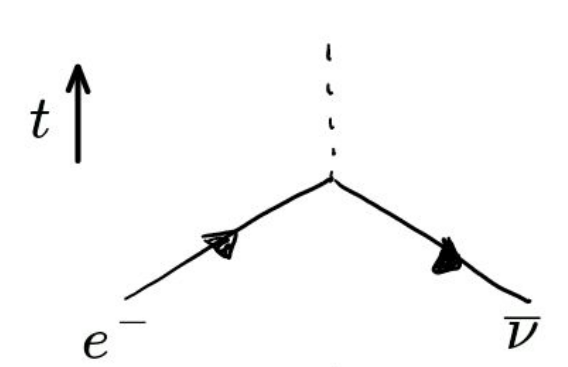
\includegraphics[scale=0.2]{images/FD_time1.png}
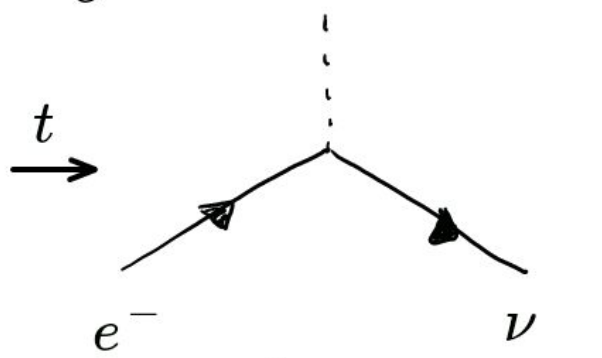
\includegraphics[scale=0.2]{images/FD_time2.png}
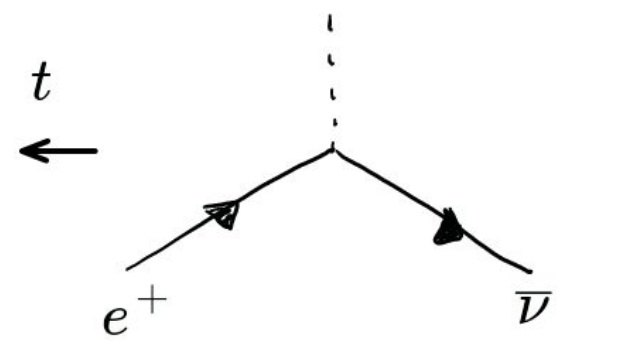
\includegraphics[scale=0.2]{images/FD_time3.png}
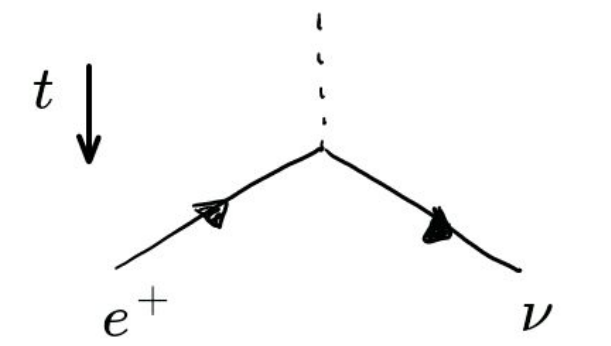
\includegraphics[scale=0.2]{images/FD_time4.png}
\end{center}
\caption{Different interpretation of a Feynman diagram for different assignments of the time direction.}\label{fig:timeDirection}
\end{figure}
On top of providing a visualisation of a process Feynman diagrams provide a recipe for calculating the amplitude for a given process. In this section we will see some of these rules.
\subsection{Fermions}
Fermions are usually represented by plain lines.  Fermion lines (in the Standard Model) cannot be interrupted, they have to start and end either in the initial or final state, or they have to be closed fermion loops. This is a reflection of the fact that the fermions carry quantum numbers that are conserved, such as electric charge, lepton number of baryon number. Fermions lines have a direction represented by arrows. If the arrow point in the time direction it represents a fermion and if it points against the time direction it represents an anti-fermion.  

\subsection{Vector bosons}

Vector bosons are typically drawn as wiggly lines for photons and W/Z bosons and  "spring" lines for gluons. You may find books or publications where dashed lines are used for weak bosons.

\subsection{Vertices}

Each vertices where particle meet represent an interaction. In most cases an interaction involves only three particles. There can only be vertices between particles which interact. In the standard model all vertices conserve the following quantities:
\begin{itemize}
\item electric charge
\item lepton number
\item baryon number ($+1/3$ for quarks, $-1/3$ for antiquarks, $0$ for all other particles)
\end{itemize}
\subsubsection{Photon}
The photon interacts with all (electrically) charged particles and does not change the flavour of the particle it interacts with.
\begin{center}
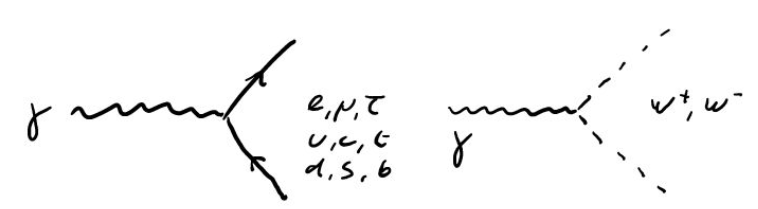
\includegraphics[scale=0.4]{images/gamma.png}
\end{center}
Each vertex of a photon with a charged particle results in a factor $Q\sqrt{\alpha}$ in the amplitude for the process (and therefore a factor of $\alpha$ in the cross section), where $Q$ is the charge of the particle and $\alpha$ is the electro-magnetic coupling strength. 
\subsubsection{$W$ boson}
The $W^+$ and $W^-$ bosons can interact with a pair of leptons or a pair of quarks. They interact with a charge lepton and its associated neutrino. In the case of quarks the interaction is between an up-type quark and a down-type quark. The interaction between quarks of the same generation is preferred, but generation changes are possible. The relative strength of the coupling between quarks is described by the CKM matrix. 
\begin{center}
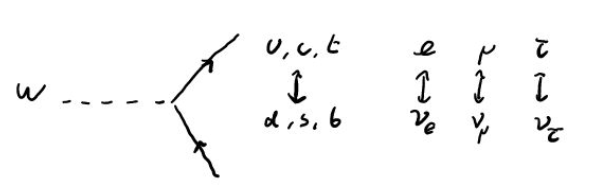
\includegraphics[scale=0.4]{images/W.png}
\end{center}
The sign of the vector boson in the above picture depends on the particles it couples to.
\subsubsection{$Z$ boson}
The $Z$ boson couples to all particles the photon couples to, and also couples to the neutrinos.
\begin{center}
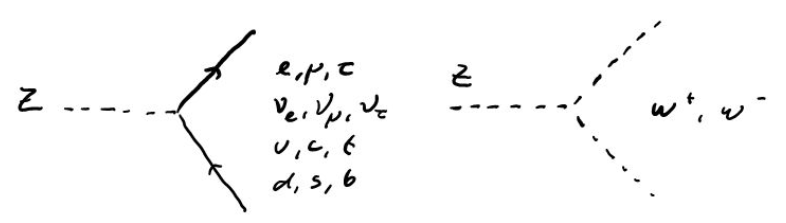
\includegraphics[scale=0.4]{images/Z.png}
\end{center}
\subsubsection{Gluon}
The gluon carries the strong interaction. It couples to all quarks and also couples to itself, as the gluon carries a colour charge. The gluon doesn't couple to leptons or to the photon, $W$, $Z$ bosons.
\begin{center}
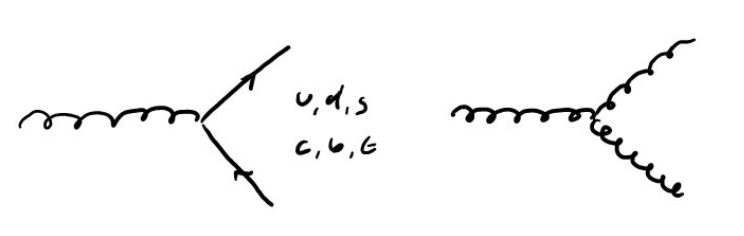
\includegraphics[scale=0.4]{images/gluon.png}
\end{center}
Each vertex of a gluon with a colour-charged particle results in a factor $\sqrt{\alpha_s}$ in the amplitude for the process (and therefore a factor of $\alpha_s$ in the cross section).

\subsection{Internal particles}

Internal lines represent virtual particles that only exist within the interaction region and are not detected. Since we don't observe what is happening in the interaction region we cannot always know in what time order particles are created and reabsorbed. Let's take the example of the scattering of an electron neutrino and a $d$ quark $\nu_e\; d\rightarrow e^-\;u$. One could see the process in two ways depicted in figure~\ref{fig:Wboth}: a) the neutrino emits a $W^+$, thereby changing into an electron, this $W^+$ interacts with the $d$ quark to give a $u$ quark b) the $d$ quark emits a $W^-$ boson and becomes a $u$ quark, this $W^-$ boson then interacts with the neutrino changing it into an electron. 
%%\image{Wboth.png}
\begin{figure}[h]
\begin{center}
\[
\parbox{0.6\textwidth}{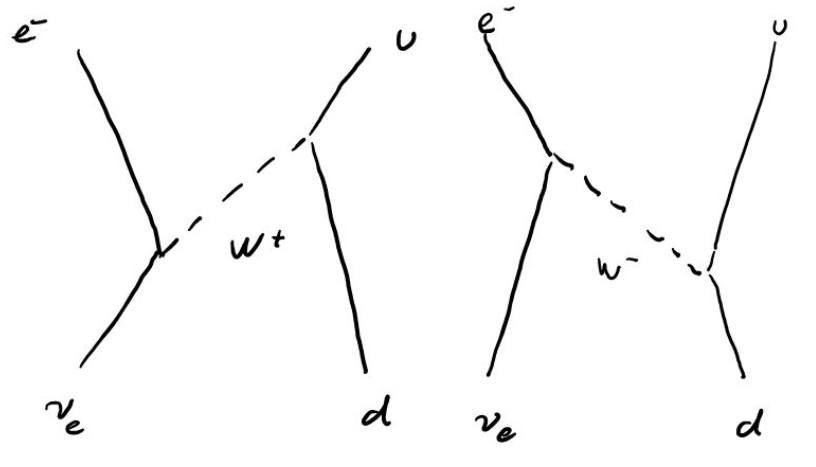
\includegraphics[scale=0.35]{images/Wboth.png}}
\Huge{\Rightarrow}
\parbox{0.3\textwidth}{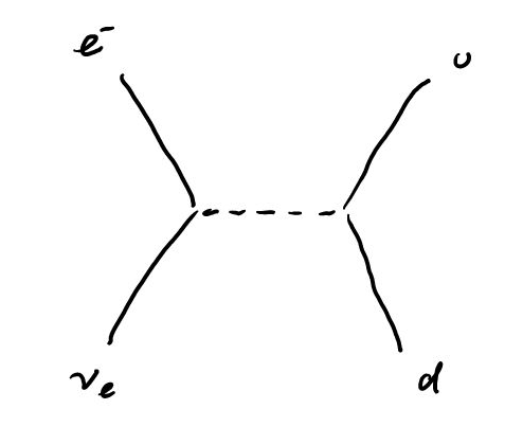
\includegraphics[scale=0.35]{images/Whoriz.png}}
\]
\end{center}
\caption{Two ways of seeing the $\nu_e\,d\rightarrow e^-\,u$ process (left) and representation of the $\nu_e\,d\rightarrow e^-\,u$ process with an horizontal vector boson (right).}\label{fig:Wboth}
\end{figure}
Since both processes happen and are indistinguishable one often represent the process using an horizontal line (when time flows vertically) as on the right side of figure~\ref{fig:Wboth}   

Internal lines bring a factor of
\[\frac{1}{p^2-m^2+im\Gamma}\]
to the amplitude of the process. $m$ is the mass of the propagating particle, $p$ the four-momentum it carries and $\Gamma$ is the decay width, it vanishes for stable particles. This factor is responsible for the resonances we observe when the invariant mass of a virtual particle is close to its "right" mass $p^2=m^2$. The width is only important in the region of $p^2$ the vicinity of $m^2$. 
\subsection{Standard model vertices}
The above list is not a complete list of ingredients for the standard model interactions, but covers what is necessary for the course. 

In the Standard model, more vertices are allowed that involves four particles at a time, but processes that involve these vertices also have Feynman diagrams which only uses three-particle interactions. There are no fundamental 4-fermion interactions (but there could be effective 4-fermion interactions such as the Fermi coupling.)
\subsection{How to draw a Feynman diagram}
Drawing Feynman diagrams for complicated process can be quite intricate, and often computer programs are used to generate all Feynman diagrams with a specific number of vertices. For simple processes in the Standard model, one possible strategy is to start with the fermion line, because in the Standard model they don't cross (because there are no four-fermion interactions). Once the fermion lines are drawn, one is left with the task of "dressing" them with the bosons. This is usually quite easy as we know which type of interactions are involved: if the flavour (and charge) of the fermion changes, a $W$ boson will be involved, if the flavour doesn't change, it will be either a photon or a $Z$ boson exchange.
%%\keypoint{All vertices in a Feynamn diagram must conserve charge, lepton numbers and baryon number.}
\clearpage
%%\lecture{17}
%%\section{Quarkonia}
\section{Quarkonia}
%%
%%
With quarkonia we denote either a \emph{charmonium} ($c\bar c$) or \emph{bottomium} ($b\bar b$) quark bound state. The top quark is so heavy that it decays before it has time to form a bound state. The advantage of the heavy $c$ and $b$ quarks is that their motion within the bound state is not relativistic. Bound states of the lighter $u,d,s$ quarks are treated in the next section. In this section we concentrate on the the charmonium, but the discussion is also valid for the bottomium.
%%\keypoint{ Bound states of a charm quark-antiquark are called charmonium, a bound state of a bottom quark and antiquark is called bottomium. We can use these states and its excited states to study the potential between a quark and an antiquark, in the same way that we can study the electromagnetic potential studying the Hydrogen atom or the positronium.}

We are going to use excitation energies of the charmonium system to investigate the binding of the two quarks. The quarkonia provide an excellent laboratory to investigate the force between a quark and an antiquark. We will label the states in the same way as the levels in the shell model: a state $n^{2S+1}L_J$ is a state corresponding to the $n$-th radial wave-function energy, with orbital angular momentum $L$, expressed as $S,P,D,F,...$ for $L=0,1,2,3,...$ This notation is different than the notation typically used for the positronium atom where the principal quantum number $N$ includes the orbital angular momentum $n_{e^+e^-}=N+L+1$.
%%\image{Charmonium.png}
\begin{figure}
\begin{center} 
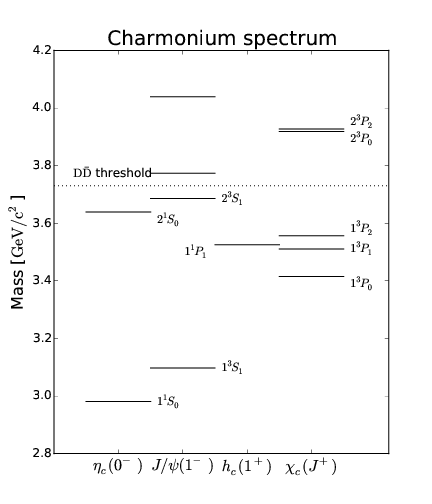
\includegraphics[scale=0.5]{images/Charmonium.png}
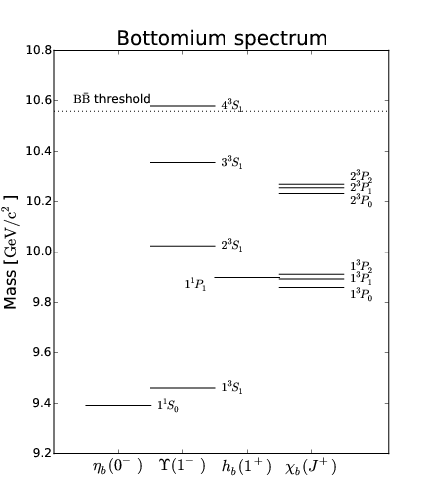
\includegraphics[scale=0.5]{images/Bottomium.png}
\end{center}
\caption{Charmonium and bottomium spectrum. The states are labelled by their spin $J$ and their parity. Data from \cite{pdg}.}\label{fig:charmonium}
 \end{figure}

Figure~\ref{fig:charmonium} shows the masses of the charmonium ($c\bar c$) and bottomium ($b\bar b$) states. The $J/\psi$ and $\Upsilon$ states have $J^P=1^{-}$ and can therefore be produced in the reaction
\[e^+e^-\rightarrow \gamma^*\rightarrow c\bar c\;,\]
because the virtual photon (denoted by $\gamma^*$) also has $J^P=1^-$. If the energy of the incoming $e^+$ and $e^-$ particles is set right the $c$ and $\bar c$ quarks produced do not have enough kinetic energy and form the charmonium bound state. The lowest $J^P=1^-$ state is called $J/\psi$. The reason for the double name is that it was discovered at the same time by two groups who gave it different names. The $J/\psi$ has a mass of $3.097\,{\rm GeV}$. 

Excited quarkonia states can decay to lower states through the emission of a photon. We will treat the decays of the quarkonia in section \ref{sec:QuarkoniaDecays}. 

Observing the spectrum of the quarkonia states allows to understand the quark-antiquark potential. We can compare this spectra with that of the positronium, shown in figure~\ref{fig:positronium}. The comparison is interesting as both states are bound states of a particle and its anti-particle.   

 \begin{figure}[h]
\begin{center} 
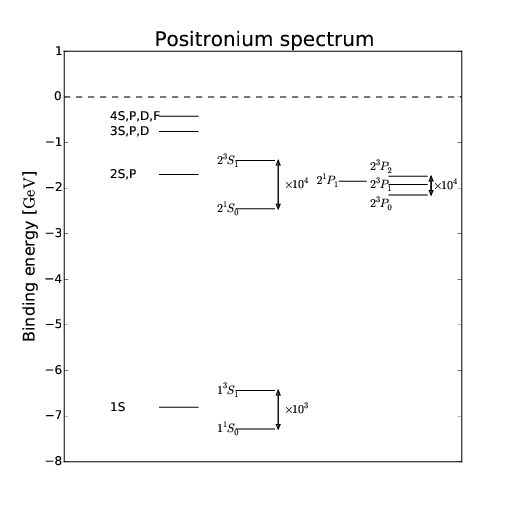
\includegraphics[scale=0.4]{images/Positronium.png}
\quad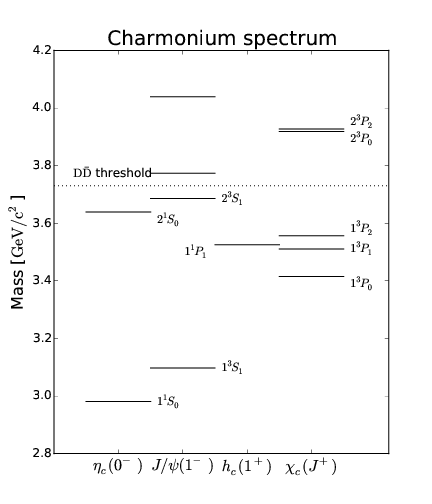
\includegraphics[scale=0.4]{images/Charmonium.png}
\end{center}
\caption{Positronium and charmonium spectra. The energy splitting in the positronium are much smaller than in the charmonium case. The energy scale has been scaled by factors of $1000$ and $10000$ to make the energy differences visible. The first column of the positronium plot shows the energy levels before including the fine and hyper-fine splittings. The positronium states are labelled using a different spectroscopy notation than the charmonium.}\label{fig:positronium}
 \end{figure}
The spectra show similarities for the lowest states. This is the case because both the potential between the two quarks has a $1/r$ behaviour for small distances (corresponding to low radial function $N$). The $2S$ and $2P$ levels in the positronium spectrum are almost degenerate, but it is not the case for the charmonium states (the 2S and 1P states in our naming convention). This is one sign of the departure from the $1/r$ behaviour of the quark-antiquark potential. Another sign of the different potential in the quarkonia bound states is that the distance between the states corresponding to different $n$ values is not shrinking as it does for the positronium spectrum. This effect a consequence of the $1/r$ potential.      
 
Comparing the spectra of the charmonium and bottomium states we see that they are fairly similar so we can conclude that the quark-antiquark potential should be mostly independent of the quark mass. 

Comparing the spectra of the positronium and that of the quarkonia in figure~\ref{fig:positronium} we see that the split between the $1^{1}S_0$ and $1^3S_1$ states is much larger in the quarkonia spectrum than in the positronium spectrum. This can be understood by considering the interaction between the spins of the two constituents of the bound state.

In the positronium state the split between the two $1S$ states originates from the spin-spin interaction. This interaction can be written as a potential
\[V_{ss}(e^+e^-)=\frac{8\pi}{3}\alpha \frac{\vec s_1\cdot\vec s_2}{m_e^2}\delta(\vec x)\;,\]
where $\vec s_i$ is the spin of particle $i$. The delta function in the potential means that this is a contact interaction: it only takes place when the two particles are at the same location. The interaction is mediated by the photon so the potential is proportional to the electro-magnetic coupling strength $\alpha\simeq1/137$. If we now want to "translate" this interaction into an interaction between two quarks under the strong force we need to change $\alpha$ into the strong coupling strength $\alpha_s$ and change the electron mass to the quark mass. The detailed calculation gives the following potential.
\[V_{ss}(q\bar q)=\frac{32\pi}{9}\alpha_s \frac{\vec s_q\cdot\vec s_{\bar{q}}}{m_q m_{\bar q}}\delta(\vec x)\;,\]    
where the different prefactor has to do with the fact that the combination of colour charges are not unity as were the product of the electron and positron electric charges. 

To obtain the mass shift in the $1S$ states we need to evaluate the expectation value of this potential in the two different spin configurations. We can calculate the expectation value of the product of the spins using
\begin{eqnarray*}
S(S+1)&=&\langle (\vec s_1 +\vec s_2)^2 \rangle\\
 &=& 
\langle \vec s_1 ^2 \rangle +2\langle \vec s_1 \cdot\vec s_2 \rangle +\langle +\vec s_2^2 \rangle \\
&=&
\frac{1}{2}\left(\frac{1}{2}+1\right)+2\langle \vec s_1 \cdot\vec s_2 \rangle + \frac{1}{2}\left(\frac{1}{2}+1\right)
\\&=&
\frac{3}{2}+2\langle \vec s_1 \cdot\vec s_2 \rangle
\end{eqnarray*}  
where we have used the fact that for spin $S$ system $\langle \vec S^2 \rangle=S(S+1)$ and the fact that the quarks have spin $1/2$ and therefore $\vec s_i^2=3/4$. We can solve to the product between the two spins:
\[\langle \vec s_1 \cdot\vec s_2 \rangle=\frac{2S(S+1)-3}{4}=\left\{\begin{array}{ccc}-\frac{3}{4}&\mbox{for}& S=0 \\ +\frac{1}{4}&\mbox{for}& S=1 \end{array}\right.\]
so that we get for the contribution $E_{ss}$ to the states mass:
\begin{eqnarray}\label{eq:1sMassSplit}
E_{ss}&=&
\langle \psi |V_{ss}|\psi\rangle = 
\frac{8\pi \alpha_s }{9m_q m_{\bar q}}\langle \psi|\delta(\vec x)|\psi\rangle \cdot\left\{\begin{array}{ccc}-3&\mbox{for}& S=0 \\ 1&\mbox{for}& S=1 \end{array}\right. \nonumber
\\
&=&
\frac{8\pi \alpha_s }{9m_q m_{\bar q}}\left|\psi(0)\right|^2 \cdot\left\{\begin{array}{ccc}-3&\mbox{for}& S=0 \\ 1&\mbox{for}& S=1 \end{array}\right. \;.
\end{eqnarray}
The mass split $\Delta E_{ss}$ between the two $1S$ states is the difference between the two values so we get
\[\Delta E_{ss}=E_{ss}(S=1)-E_{ss}(S=0)=\frac{32\pi}{9}\frac{\alpha_s }{m_q m_{\bar q}}\left|\psi(0)\right|^2\;.\]
Since the energy split is proportional to the wave function at the origin, this contribution is mostly relevant for the radial wave function with the lowest energy.
%%\keypoint{The large splitting of the $L=0$ quarkonia states is due to a spin-spin interaction.}

The mass of the quarks entering this formula is the so-called \emph{constituent} mass. The quarks have their own mass but when they are in a bound state they are surrounded by a cloud of gluons and quark-antiquark virtual particles, so their "effective" mass, the constituent mass, is larger.  
\subsection{Quark-anti-quark potential}
From the previous discussion we have seen that we expect the short distance potential between the quark to have a similar $1/r$ behaviour as the electro-magnetic potential in the positronium, but that the larger $r$ behaviour should be different. As the energy levels do not display the same compression as they do in the positronium spectrum we expect the potential not to be bounded. We can make the following ansatz:
\[V(r) = \underbrace{-\frac{4}{3}\frac{\alpha_s(r)}{r}}_{\mbox{short-range}}
+\underbrace{kr}_{\mbox{long-range}}\;.
\]  
%%\keypoint{At small distances $r$ the $q\bar{q}$ potential behaves as $1/r$ but it is not a pure $1/r$ potential: we have an additional term linear in the distance which leads to confinement.}
\begin{figure}
\begin{center}
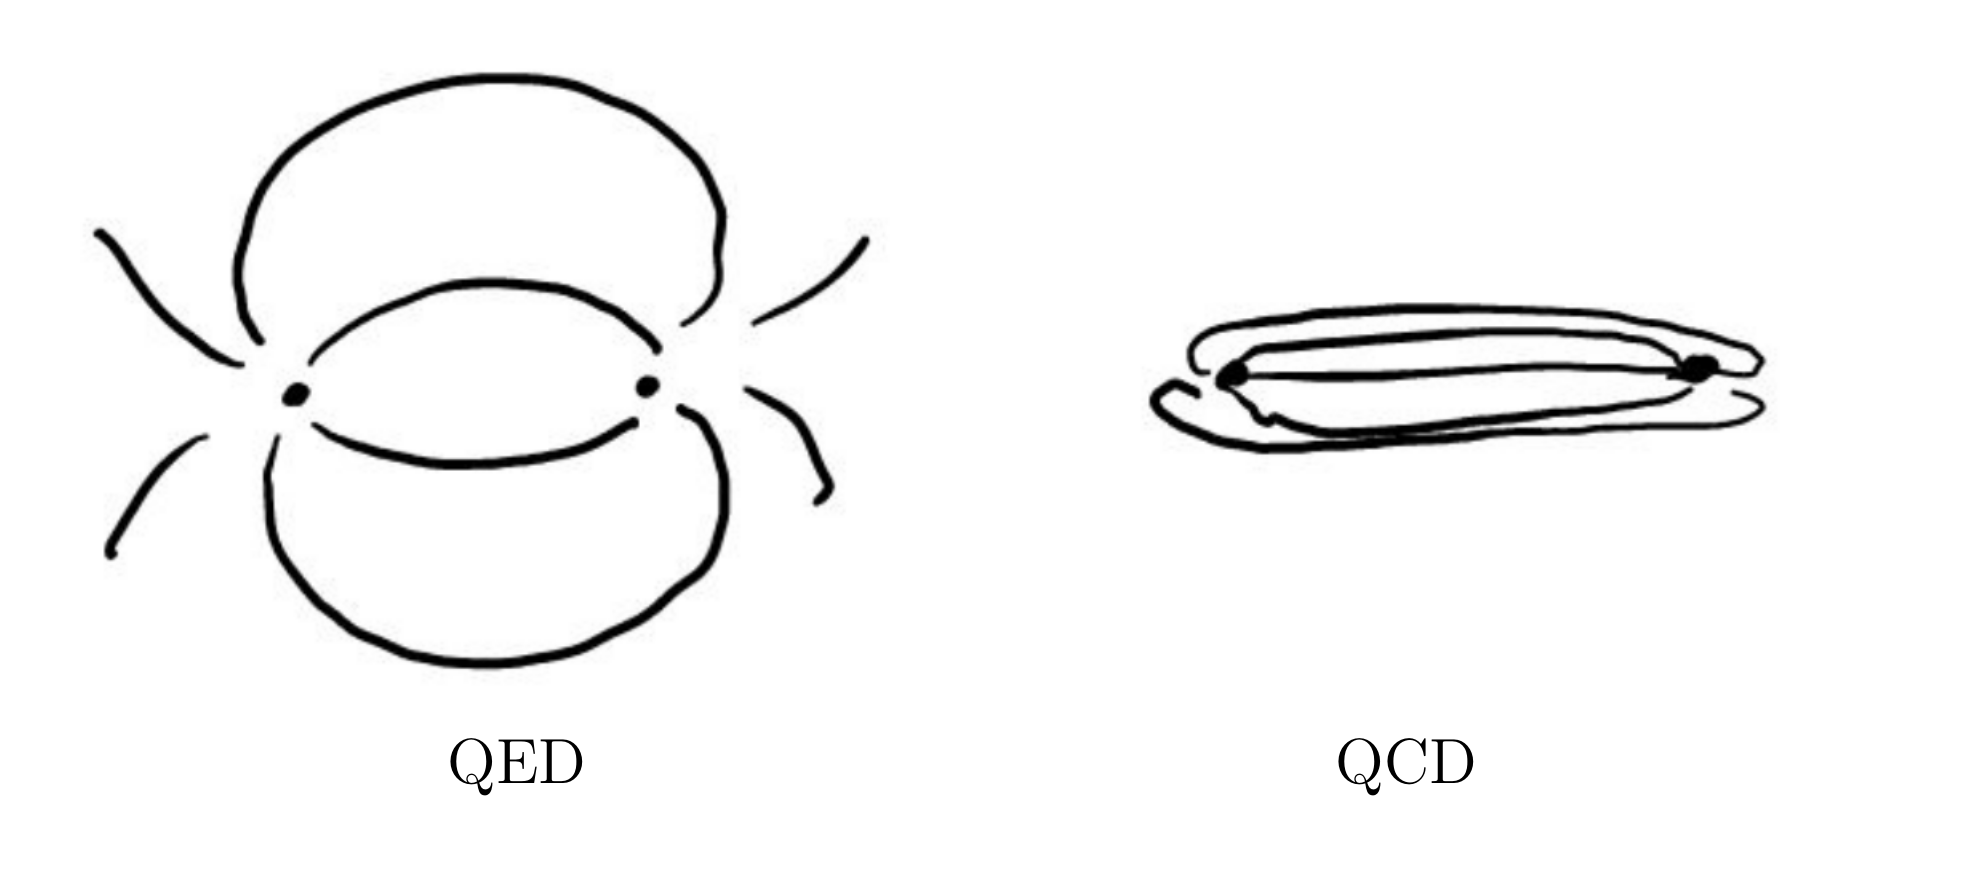
\includegraphics[scale=0.2]{images/QEDQCD_withlabel.png}
\end{center}
\caption{Schematic depiction of the field lines for the electro-magnetic potential (left) and the quark-antiquark potential (right). Due to the self interaction of the gluons the field lines attract each other and form a "flux tube".}\label{fig:fieldLines}
\end{figure}
The first term is the short-range interaction that is similar to the electro-magnetic interaction, the prefactor $4/3$ has to do with the fact the colour charges are not simply $1$ as in the QED case. For larger distances the potential increases linearly. We can build an intuitive picture by plotting the field line of the electro-magnetic and strong force between two charges, as depicted in figure~\ref{fig:fieldLines}. The strong force field lines attract each other due to the self-interaction of the gluons and forms a "flux tube". Pulling the quarks apart stretches this flux tube and the energy stored in the flux tube increases linearly with the distance. The constant $k$ in the above ansatz is called the string tension. 

We can use this potential and predict the spectrum of the quarkonia. Comparing this prediction with the measured spectrum we can find the values of the parameters $\alpha_s(r)$ and $k$. This simple model gives reasonable agreement with the observations. Typical values obtained are 
\[\alpha_s\simeq 0.15-0.25\;,\quad k\simeq 1\,{\rm GeV/fm}\;,\quad m_c\simeq1.5 \,{\rm GeV}\;.\] 
One consequence is that if we try to stretch apart a quark and an antiquark we store more and more energy in the flux tube between them and at some point (around $1\,{\rm fm}$) there is enough energy to create a new quark-antiquark pair. So unlike two electric charges where there is a fixed amount of energy needed to separate two charges it is not really possible to separate colour charged particles.  
\begin{figure}
\begin{center}
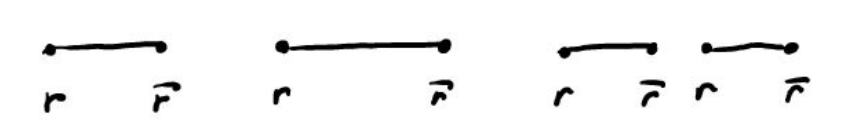
\includegraphics[scale=0.4]{images/hadronisation.png}
\caption{When pulling a quark and an anti-quark apart we need so much energy that it becomes energetically favourable to create a new quark-antiquark pair to "break" the field tube between the two colour charges.}\label{fig:hadronisation}
\end{center}
\end{figure} 
%%\lecture{18}
%%\section{Quarkonia decays}
\subsection{Quarkonia decays}\label{sec:QuarkoniaDecays}
%%
%%  
Quarkonia are not stable particle and have four ways of decaying.
\subsubsection{Electro-magnetic decay to lower states}
Excited quarkonia can decay into lower lying states through photon emission. As for excited states of nuclei there are two different modes: electric or magnetic. Which one is allowed depends on the parity of the initial and final states. Since the parity of a state is given by the product of the intrinsic parities and the parity of the spatial wavefunction. For a quarkonium state $n^{2S+1}L_J$ the parity is given by 
\[P(n^{2S+1}L_J)=P(q)P(\bar q)(-1)^L=(-1)^{L+1}\;,\]
where we have used the fact that the intrinsic parities of a fermion and anti-fermion are opposite, so that the product of the parities $P(f)P(\bar f)$ is always $-1$.  

The selection rules are the same as for the decay of nuclear excited states: electric transitions with multipolarity $\ell$ has parity $(-1)^\ell$ and a magnetic transition has parity $(-1)^{\ell+1}$. An electric transition is triggered by a change in the orbital angular momentum of the state and a magnetic transition is triggered by a change in the spin configuration of the quarks.

If we restrict our discussion to $E1$ and $M1$ transitions the electric transition occur between states of different parities and magnetic $M1$ transition occur between states of the same parity. For example for the decay
\[2^{3}S_1\rightarrow  1^3P_{J}\;,\quad J=0,1,2\]
we have an initial total angular momentum $J_i=1$. If we have a $\ell=1$ transition the total final state angular momentum will be the (vector) sum of $\ell$ and $J$ so the allowed values of $J$ satisfy
\[|J_i-\ell|\leq J \leq J_i+\ell \]
which is $0\leq J\leq 2$ in our case. Because we go from a state with negative parity to a state with positive parity the transition has to be electric. 

The transition
\[2^{3}S_1\rightarrow  1^1S_0\;,\]
on the other hand is between states of equal (negative) parity so it can occur through a magnetic transition $M1$. There can be no transitions between $2^{3}S_1$ and $1^{3}S_1$ because neither the spin nor the angular momentum is changed. This can be understood in the following way. A change of radial wave function for the bound state only changes the charge distribution within the bound state. Because of Gauss law such a change does not change the field outside of the bound state, so no electromagnetic wave can be generated by a pulsating radial charge distribution.  
    

\subsubsection{Annihilation into virtual photons or gluons}
The charmonium state is a bound state between a particle and its antiparticle, they can annihilate and produce either an off-shell photon, two on-shell photons or two gluons. The off-shell photon will decay into either in a pair of leptons ($e^+e^-,\mu^+\mu^-$) or into a pair of quarks (which will produce hadrons). The allowed decay modes depend on the total angular momentum of the charmonium state:
\begin{description}
\item[$\mathbf{J=0}$:] an example is the $\eta_c$ particle which corresponds to the $1^{1}\,S_0$, it can decay in the following channels:
\begin{center}
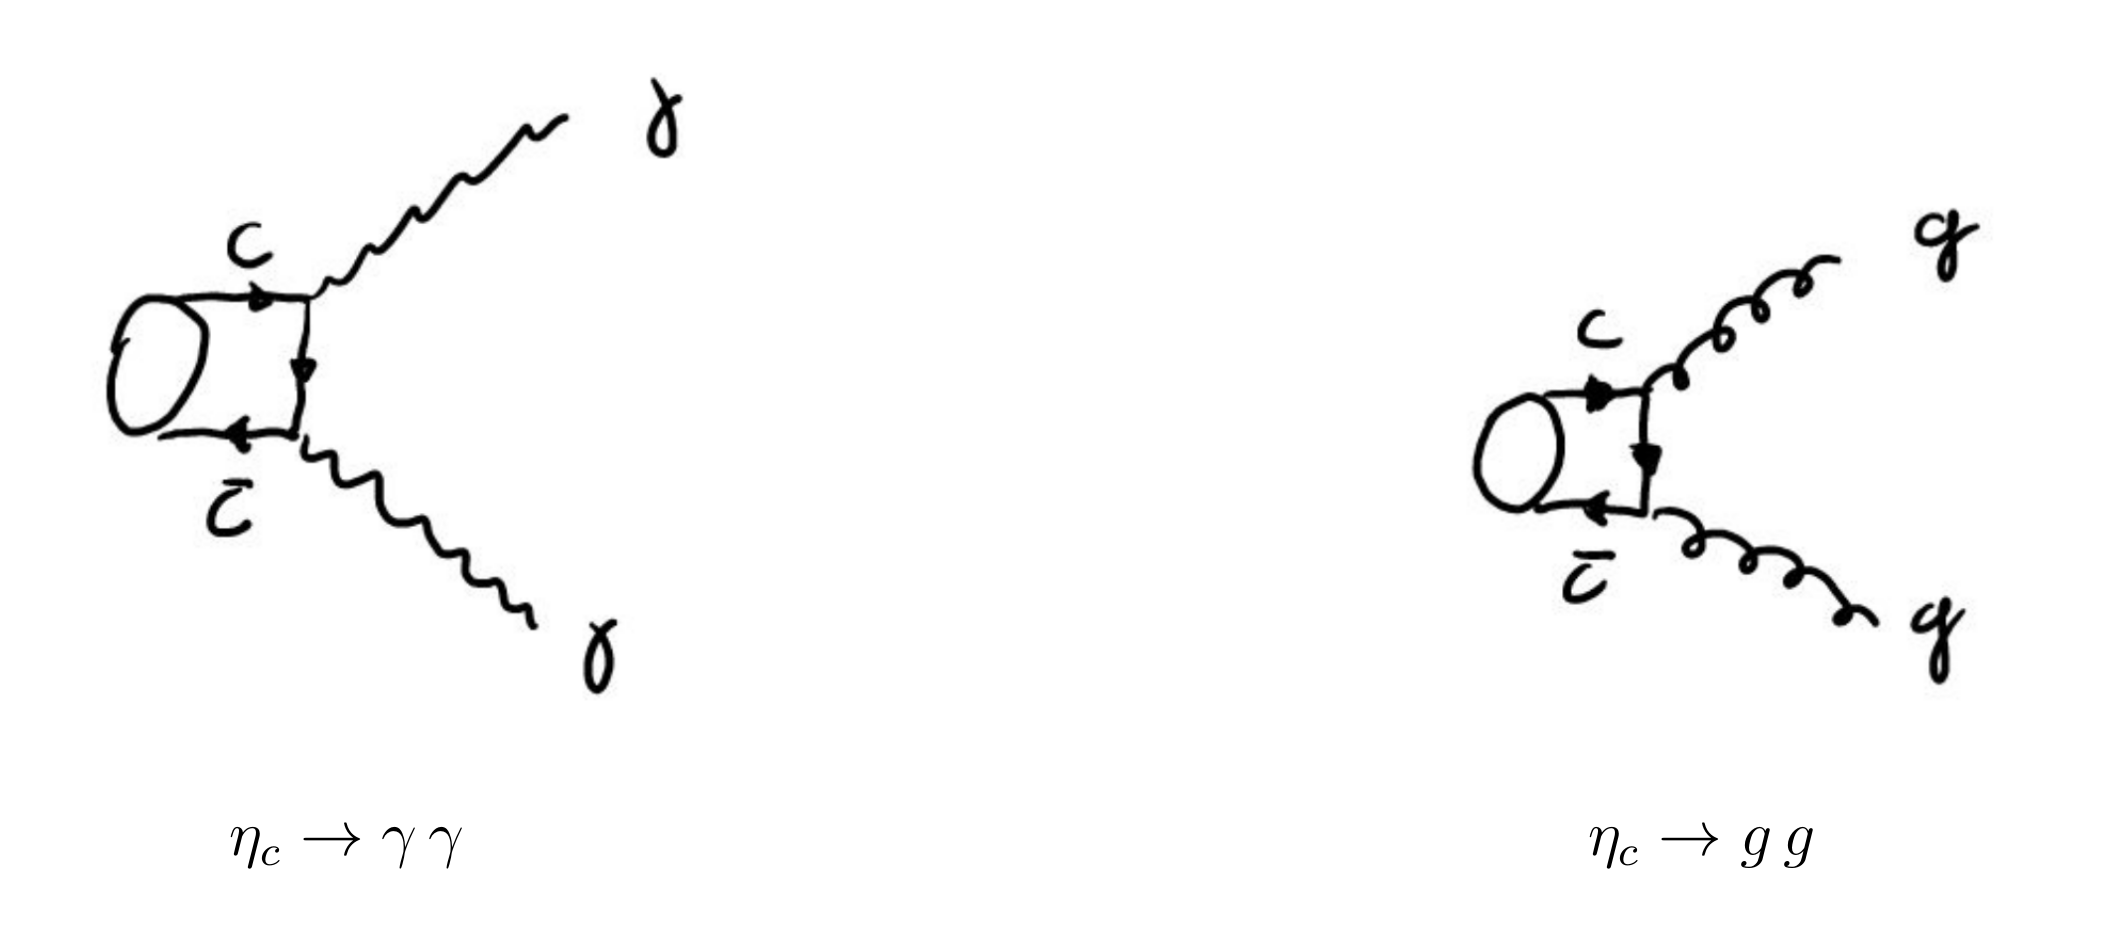
\includegraphics[scale=0.2]{images/etacgammagammagg.png}
\end{center}
The decay through a virtual photon is not possible since an off-shell photon has spin $1$ and angular momentum would not be conserved in the decay of the $\eta_c$ particle that has total angular momentum $J=0$.
\item[$\mathbf{J=1}$:] The $J/\psi$ is the charmonium state $1^{3}\,S_1$. It can decay into an off-shell photon, three photons or three gluons. 

\begin{center}
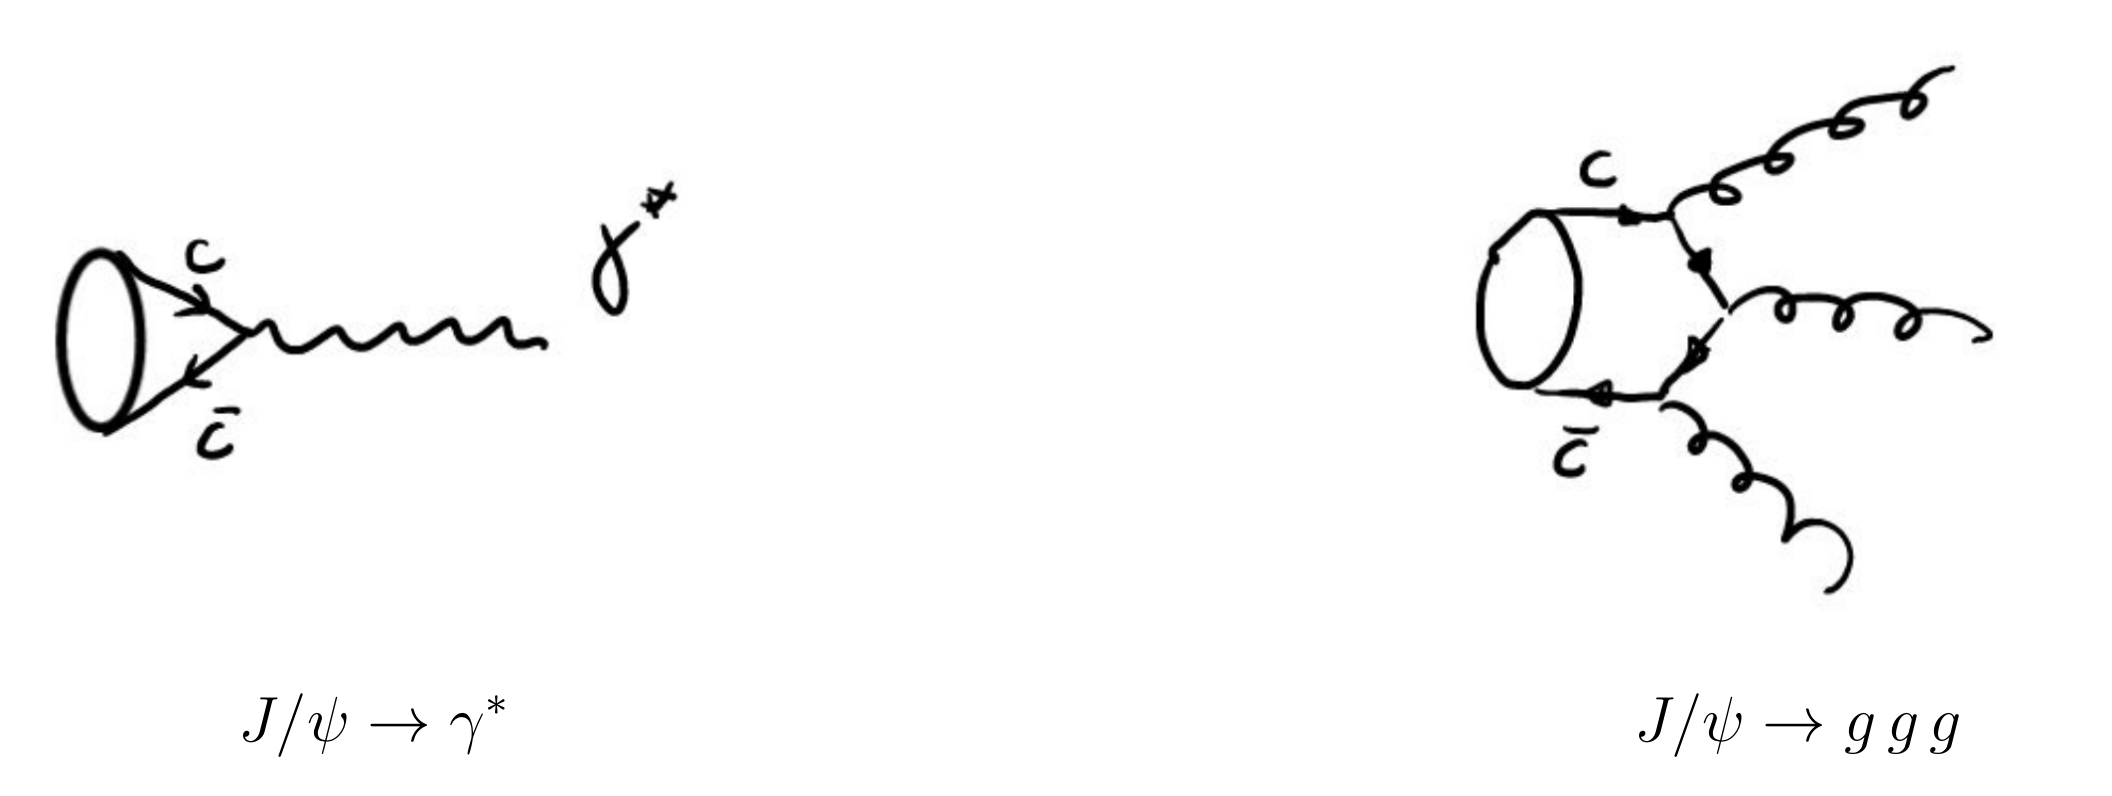
\includegraphics[scale=0.2]{images/jpsigammastarggg.png}
\end{center}
The decay into two photons of gluons is not allowed because of charge conjugation parity conservation. The decay into a single gluon is not allowed because the charmonium is colour and the gluon carries a colour-anticolour charge, so such a decay would not conserve colour charge.   
\end{description}  

\subsubsection{Decay through creation of a quark-antiquark pair}
The charmonium state is bound by the strong force, and as in the case of the proton, there can be virtual pairs of quark-antiquark produced within the bound state and if the bound state is heavy enough such a quark-antiquark pair can be used to create two new mesons, as illustrated below  
\begin{center}
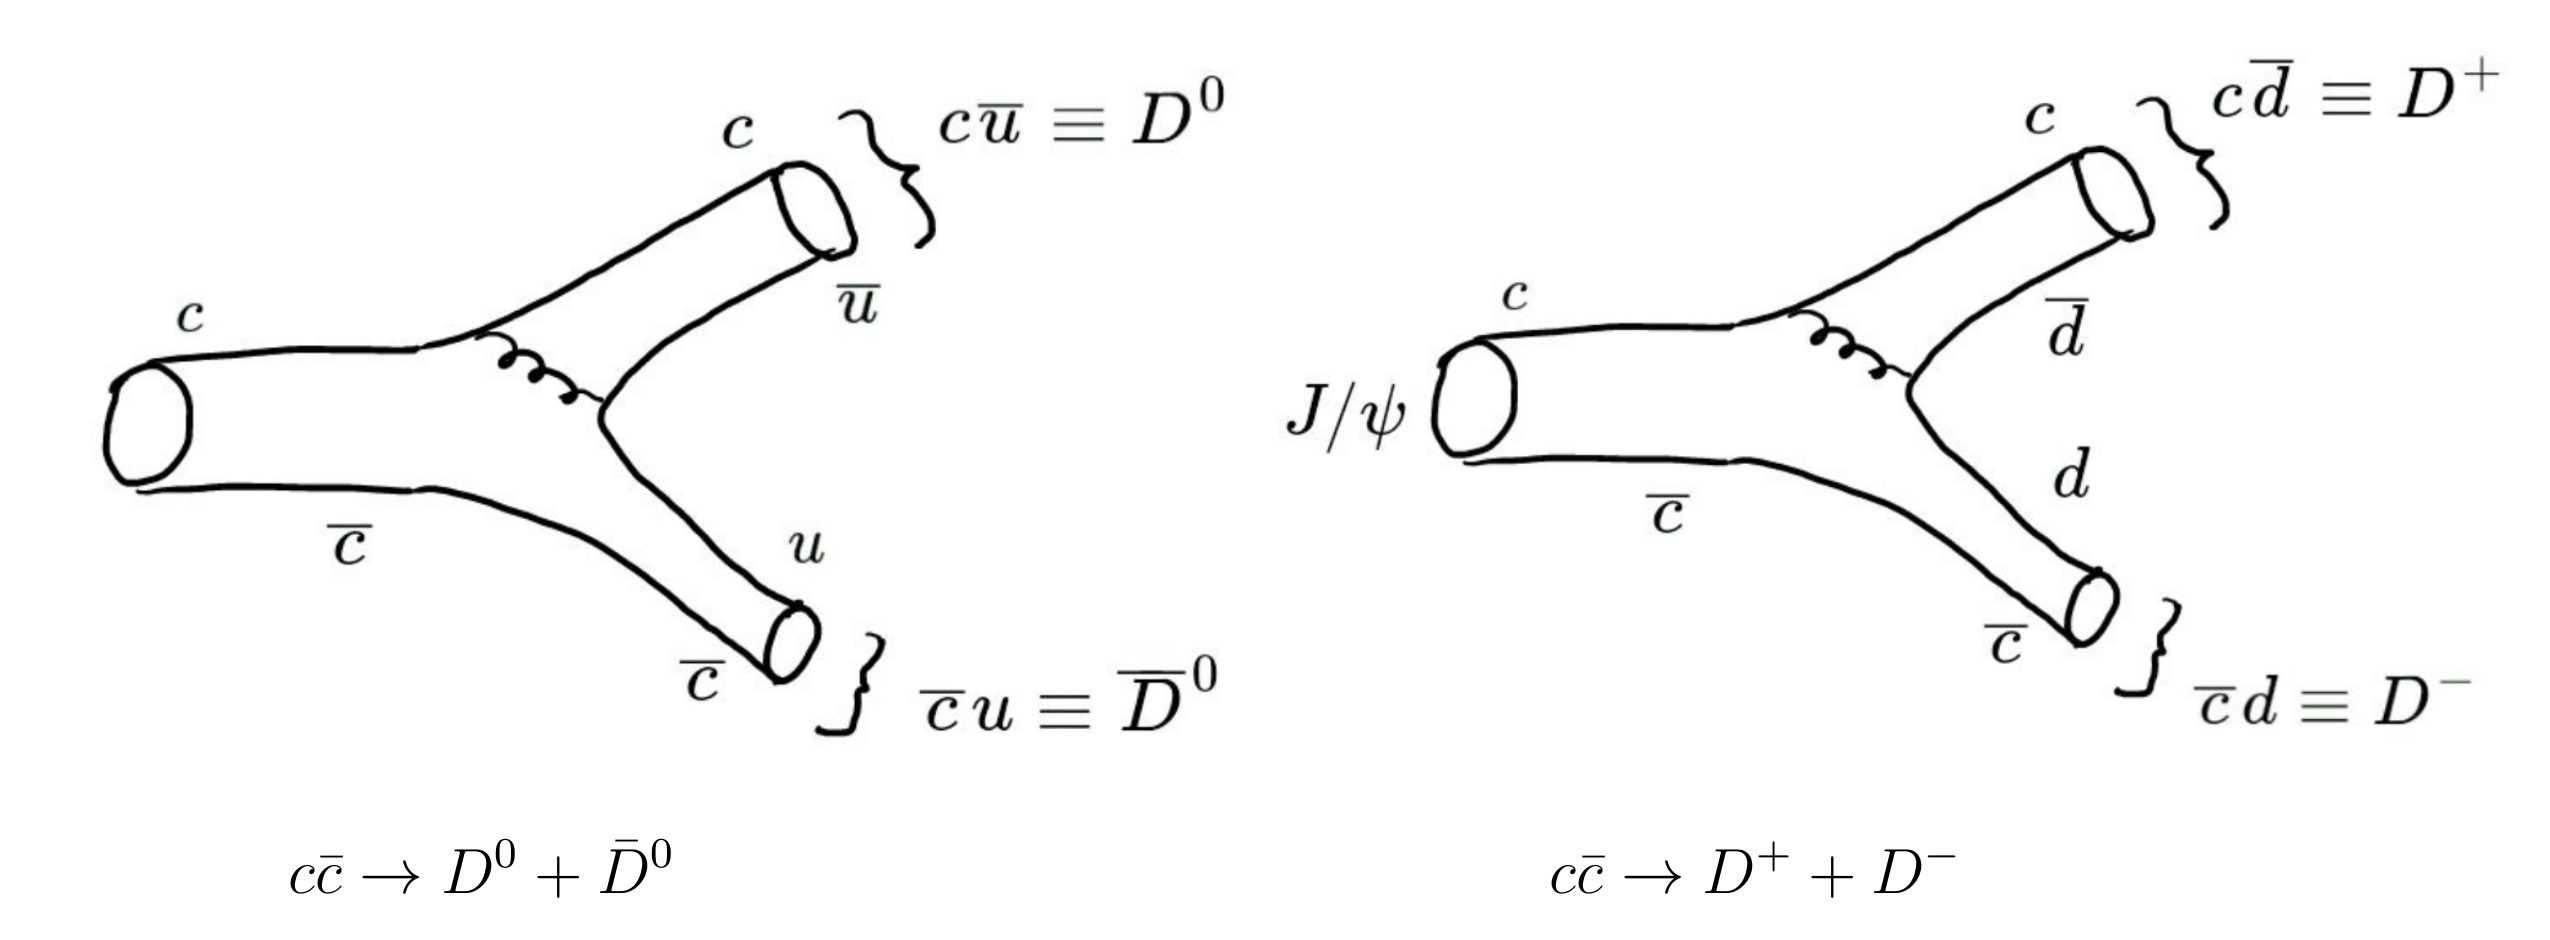
\includegraphics[scale=0.2]{images/ccdd.png}
\end{center}
This kind of decays are only possible if the sum of the masses of the new mesons is smaller than the mass of the parent quarkonium. This is not the case for the lowest states of the charmonium and bottomium, but is possible for higher states. The threshold for this type of decays is shown in the spectra in figure~\ref{fig:charmonium}. 
\subsubsection{Weak decay}
The heavy quarks in the charmonium can also decay into lighter quarks through the weak interaction. In this decay one of the heavy quarks emits a $W^\pm$ boson and change into a lighter quark. The $W$ boson subsequently decays into a lepton pair or a quark-antiquark pair. 
%%\image{charmoniumDecay5.png}
\begin{center}
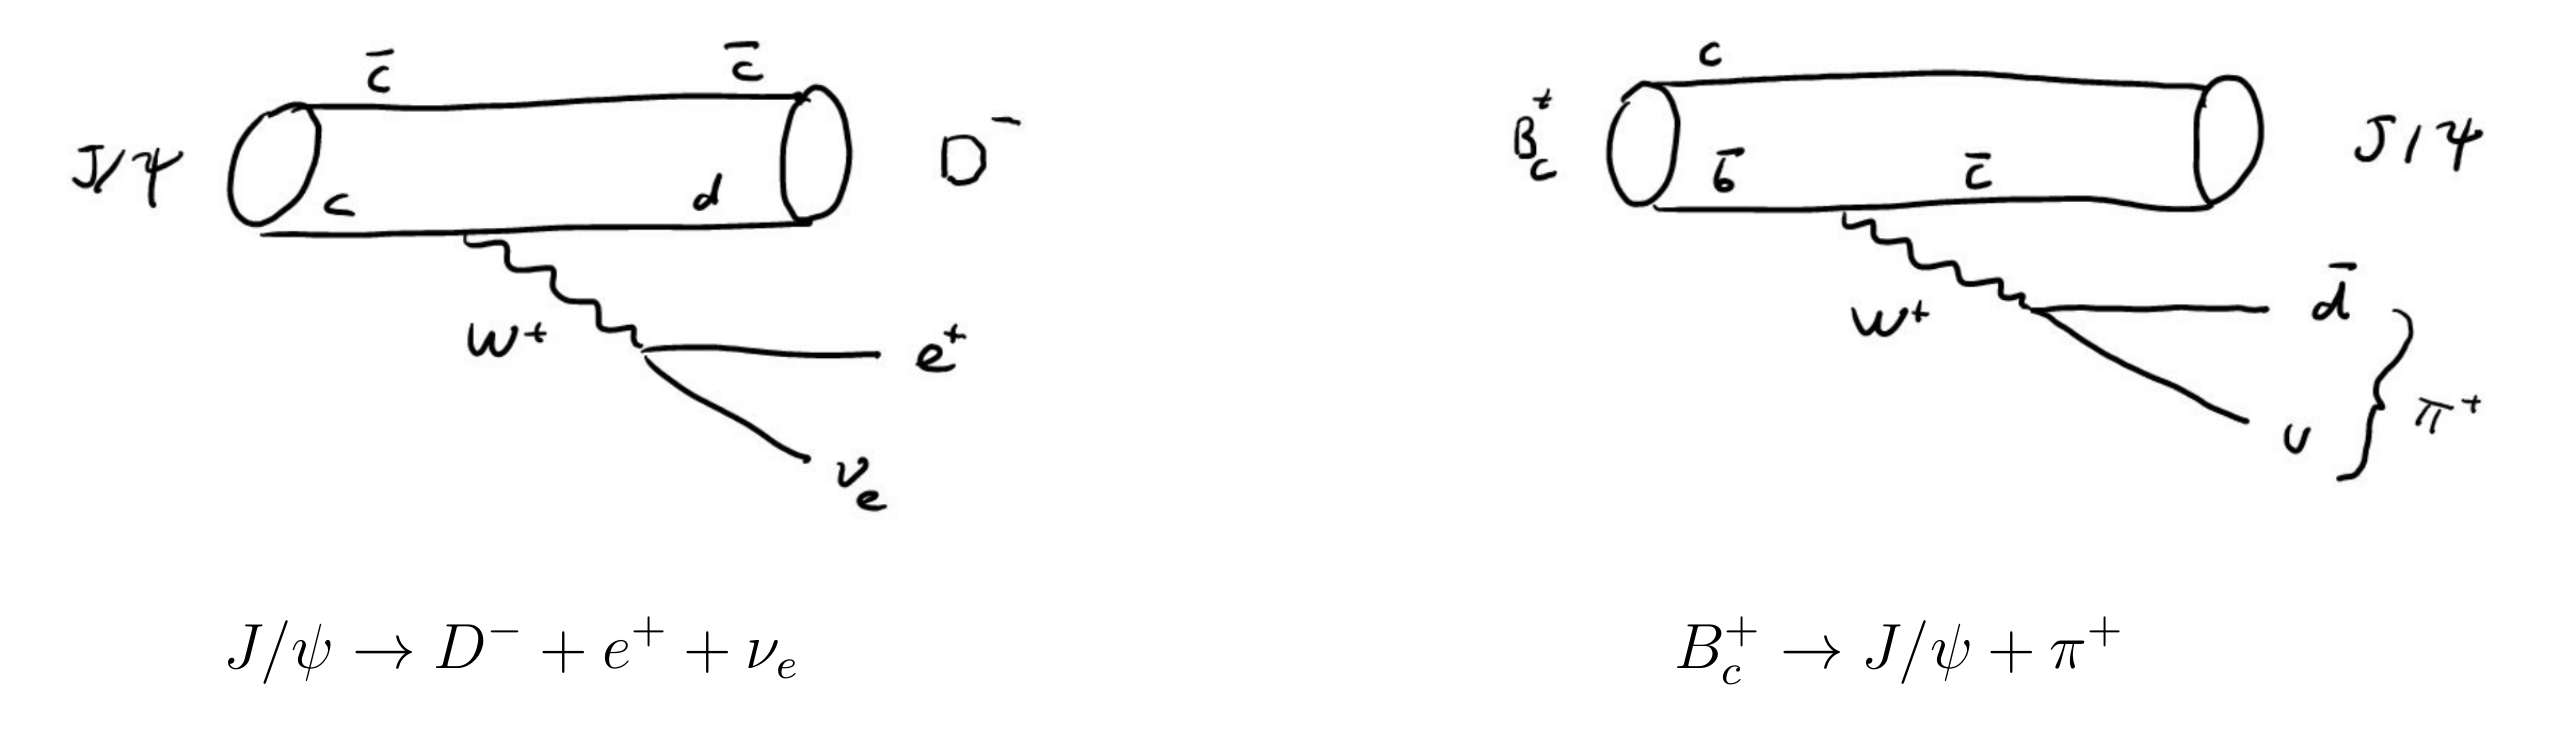
\includegraphics[scale=0.2]{images/jpsiWeak.png}
\end{center}
%%\keypoint{Quarkonia states can decay in four ways: (a) decay into a lower state through emission of a photon, (b) annihilation of the $q\bar{q}$ pair into an off-shell photon (which subsequently decays into, for example, a lepton pair) or several real photons, (c) decay into several hadrons through the creation of a $q\bar{q}$ pair from the vacuum and recombination of the $c$/$b$ quarks with them into mesons, (d) Weak decay of the heavy ($c$,$b$) quark into a lighter quark.}

%%\lecture{19}
\subsection{Relative strength}
If kinematically possible the decay through the creation of a new quark-antiquark pair is the most likely as it is caused by the strong interaction.

The value of the thresholds is given by the masses of the $D$ and $B$ mesons 
$m_{D^0}=m_{\bar D^{0}}\simeq 1864.8 \,{\rm  MeV}$,
$m_{D^+}=m_{D^{-}}\simeq 1869.6 \,{\rm  MeV}$,
$m_{B^0}=m_{\bar B^{0}}\simeq \,{\rm  5279.2 MeV}$,
$m_{B^+}=m_{ B^{0}}\simeq 5279.5\,{\rm  MeV}$.

\[c\bar c \;\rightarrow\; \underbrace{c\bar u}_{D^0}+\underbrace{\bar c u}_{\bar D^0}\qquad \mbox{threshold: } 3.7296\,{\rm  GeV}\]
\[c\bar c \;\rightarrow\; \underbrace{c\bar d}_{D^+}+\underbrace{\bar c d}_{D^-}\qquad \mbox{threshold: } 3.7392\,{\rm  GeV}\]
\[b\bar b \;\rightarrow\; \underbrace{b\bar d}_{B^0}+\underbrace{\bar b d}_{\bar B^0}\qquad \mbox{threshold: } 10.5584\,{\rm  GeV}\]
\[b\bar b \;\rightarrow\; \underbrace{b\bar u}_{B^-}+\underbrace{\bar b u}_{B^+}\qquad \mbox{threshold: } 10.559\,{\rm  GeV}\]

The decay through a virtual photon or several gluons come next. The virtual photon decay channel uses the electro-magnetic interaction which is weaker than the strong force. It can compete with the decay through several gluons because in the latter case more than one power of the coupling strength is needed as more than one gluon is emitted.

Since the weak decay is mediated through the weakest interaction it is very slow and is quite difficult to measure if other decay channels are available. It is only relevant in cases where other decays are not allowed. 

\clearpage
%%
%%\section{Light quark mesons}
\section{Light quark mesons}
%%
%%
Mesons containing $u$, $d$ and $s$ quarks are more difficult to describe than for the quarkonia because their motion within the bound state is relativistic due to their their small mass and because the masses of the three quarks are close to each other which makes the identification of patterns more tedious.
%%\keypoint{Mesons are bound states of a quark and an anti-quark, normally involving the light quarks $u$,$d$ and $s$. We only consider the states with no orbital angular momentum ($L=0$).}
%
%
\subsection{properties of the mesons} 
%%
We will only consider the lowest $L=0$ meson states leaving out the higher $n$ and $L$ bound states. This means we restrict ourselves to $1S$ states. The parity of these states is given by the product of the intrinsic parities and the parity of the two-body wave function:
\[P=P(q)P(\bar q)(-1)^L=-P(q)P(\bar q)=-1\;,\] 
where we have used the fact that the intrinsic parities of a fermion and its anti-fermion are opposite. For a $L=0$ state composed of two spin $1/2$ particles we have the two possibilities $J=0$ or $J=1$ for the total angular momentum $J$ of the bound state (which is the spin of the bound-state). In both cases the parity is negative so we have states with:
	\begin{itemize}
	\item $J^P=0^-$, they are called pseudo-scalar mesons. "Scalar" because its spin is $0$ and "pseudo" because the usual behaviour of scalars is not to change under space inversions.
	\item $J^P=1^-$, they are called vector mesons. "vector" because they have spin $1$ and no "pseudo" because getting a minus sign under parity transformation is the usual behaviour for a vector.
	\end{itemize}
%%\keypoint{There are two types of mesons, pseudo-scalar mesons which have spin $0$ and vector mesons that have spin $1$.}
%%\keypoint{Mesons have negative parity (for the $L=0$ states we are considering)}
Since we have three light quark flavours and three antiquark flavours we expect 9 different meson combinations. The strong force does not distinguish between the $u$, $d$ and $s$ quarks. We have seen that it does not distinguish between the $u$  and $d$ quarks and have called this symmetry "isospin" symmetry, we will describe it more precisely below. In the context of light quark mesons we now extend this symmetry to all transformations that mix the three light flavours between each other. We call this symmetry the flavour $SU(3)$ symmetry. 

We have already encountered a symmetry between three objects in the context of the three colour charges of the quarks. It is referred to as $SU(3)$ colour symmetry and the two applications of this same $SU(3)$ group in the two different contexts should not be confused.

Because the strange quark is more different than the $u$ and $d$ quarks we also introduce a quantum number to help characterise the strange content of the mesons: the strangeness. The strangeness is an additive quantity. For historical reasons the strangeness is defined as 
\[S=-1\; \mbox{for a $s$ quark}\;,\quad S=+1 \;\mbox{for an $\bar s$ antiquark}\;.\]   
Strangeness is conserved by the electro-magnetic and strong forces, but is violated by the weak interactions. 
%%\keypoint{We introduce the strangeness quantum number. It is additive, $s$-quark have strangeness $-1$ and $\bar{s}$-quarks have strangeness $+1$. All other quarks have strangeness $0$.}
\subsubsection{Isospin}
The $u$ and $d$ quarks are identical as far as the strong force is concerned, but are different for the electro-magnetic force. We use this symmetry under the strong force to describe strong processes. We have two states $u$ and $d$ that can, as far as the strong force is concerned, be rotated without changing the physics. It is the same situation as with a spin where we have two states that are indistinguishable, as long as no magnetic field is present. The spin described the behaviour of states under spacial rotations, isospin describes the behaviour of states under a rotation in $u$-$d$ space. The isospin is described by the same operators as the spin:
\[
I_1=\frac{1}{2}\left(\begin{array}{cc}0&1\\1&0\end{array}\right)\;,\quad
I_2=\frac{1}{2}\left(\begin{array}{cc}0&-i\\i&0\end{array}\right)\;,\quad
I_3=\frac{1}{2}\left(\begin{array}{cc}1&0\\0&-1\end{array}\right)\;,\quad
\]
As for the spin we have the square of the isospin operator:
\[I^2=I_1^2+I_2^2+I_3^2\]
with eigenvalues of the form $I(I+1)$ where $I$ is an integer or an half integer. The isospin has the same addition rules as the the spin, for example the sum of two isospin $1/2$ can be either in an $I=1$ isospin triplet of state or in an $I=0$ isospin singlet. The basis is chosen such that $I_3$ is diagonal. The $u$ and $d$ quarks form an isospin doublet
\[\left(\begin{array}{c}u\\d\end{array}\right)\;,\qquad I_3 =\left\{\begin{array}{c}+1/2\\-1/2\end{array}\right.\;\qquad I=1/2\;.\]
the $\bar u$ and $\bar d$ antiquarks also build an isospin doublet:
\[\left(\begin{array}{c}-\bar d\\\bar u\end{array}\right)\;,\qquad I_3 =\left\{\begin{array}{c}+1/2\\-1/2\end{array}\right.\;\qquad I=1/2\;.\]
 
\subsection{Meson multiplets}
In appendix~\ref{sec:Symmetries} we show that the combination of a quark belonging to a flavour triplet $\mathbf{3}$ and an antiquark belonging to a triplet $\mathbf{\bar 3}$ give two sets of states:
\[\mathbf{3}\otimes \mathbf{\bar 3} = \mathbf{8}\oplus \mathbf{1}\;\] 
that is an octet of states transforming into each other under flavour rotations and one singlet state that is invariant under flavour transformations. This picture would be more apparent if the symmetry between the three flavours was perfect. It is not the case as the masses of the $u$  and $d$ quarks are closer to each other than that of the $s$ quark. The less broken symmetry between the $u$ and $d$ quarks is a sub-group of the $SU(3)$ flavour symmetries and we can use it to refine the categorisation in the octet. 
%%keypoint{We can use the approximate symmetry between $u$, $d$ and $s$ quarks to organise the meson spectrum.}

Figure~\ref{fig:mesonOctetJ0} shows the nine pseudo-scalar mesons in the plane of the third component of the isospin and the strangeness. We see that we obtain one isospin triplet, two isospin doublets and an isospin singlet.

Figure~\ref{fig:mesonOctetJ1} shows the same plot for the vector mesons. We see almost the same pattern, with one notable difference: the two states with $I_3=0$ and $S=0$, one from the flavour octet and the flavour singlet mix to form the two physical states $\omega$ and $\phi$. This is allowed because flavour is only an approximate symmetry. 

%%\image{MesonOctetJ0.png}
\begin{figure}[h]
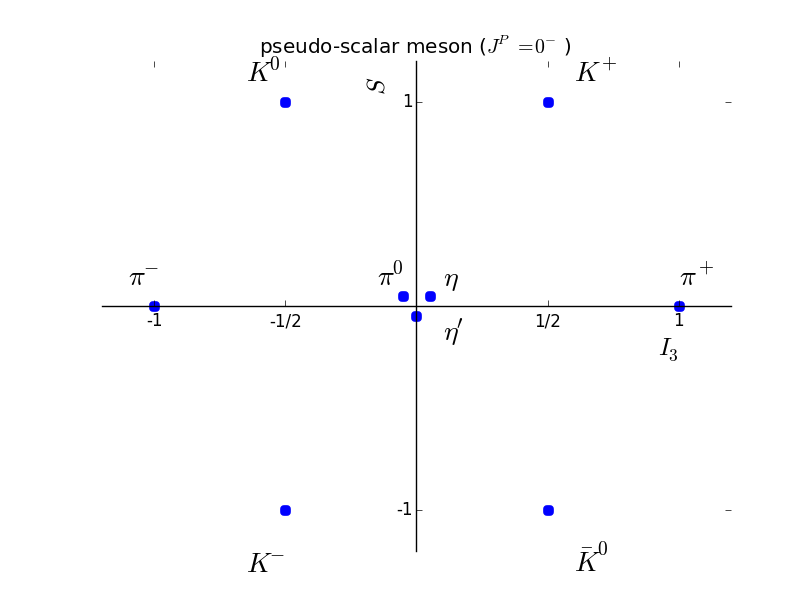
\includegraphics[scale=0.75]{images/MesonOctetJ0.png}
\caption{Pseudo-scalar mesons in the $I_3/S$ plane.}\label{fig:mesonOctetJ0}
\end{figure}
Flavour octet:
\[\begin{array}{l}
\left.\begin{array}{ccc}
\left|\pi^+\right>&=&\left|u\bar d\right>\\
\left|\pi^-\right>&=&\left|d\bar u\right>\\
\left|\pi^0\right>&=&\frac{1}{\sqrt{2}}\left(\left|u\bar u\right>-\left|d\bar d\right>\right)
\end{array}
\right\} \; I=1,\;S=0\\
%%
\left.\begin{array}{ccc}
\left|K^+\right>&=&\left|u\bar s\right>\\
\left|K^0\right>&=&\left|d\bar s\right>\\
\end{array}
\right\}\;  I=1/2,\;S=+1\\
%%
\left.\begin{array}{ccc}
\left|K^-\right>&=&\left|s\bar u\right>\\
\left|\bar K^0\right>&=&\left|s\bar d\right>\\
\end{array}
\right\}\; I=1/2,\;S=-1\\
\left.\begin{array}{ccc}
\left|\eta\right>&=&\frac{1}{\sqrt{6}}\left(\left|u\bar u\right>+\left|d\bar d\right>-2\left|s\bar s\right>\right)\\
\end{array}
\right\}\; I=0,\;S=0
\end{array}
\]
Flavour singlet:
\[\left|\eta'\right>=\frac{1}{\sqrt{3}}\left(\left|u\bar u\right>+\left|d\bar d\right>+\left|s\bar s\right>\right)\]
\clearpage
\begin{figure}[h]
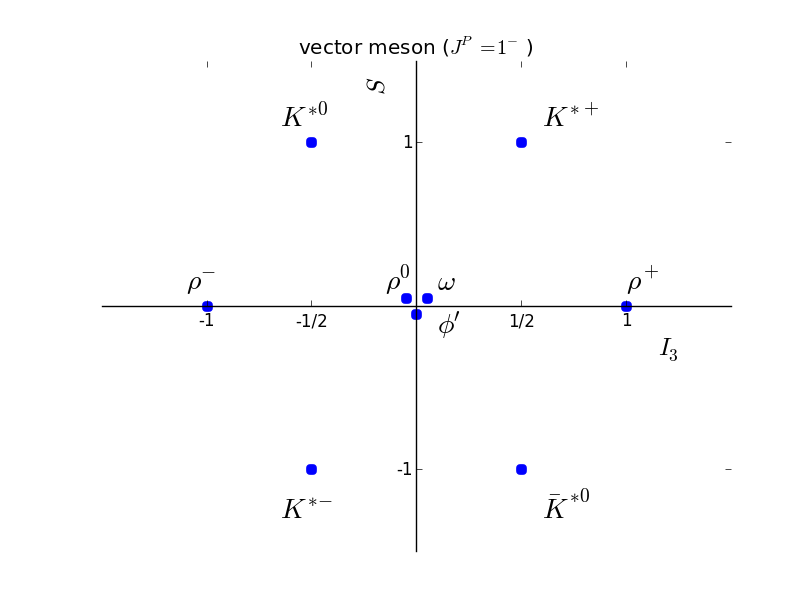
\includegraphics[scale=0.75]{images/MesonOctetJ1.png}
\caption{Vector mesons in the $I_3/S$ plane.}\label{fig:mesonOctetJ1}
\end{figure}
Flavour octet:
\[\begin{array}{l}
\left.\begin{array}{ccc}
\left|\rho^+\right>&=&\left|u\bar d\right>\\
\left|\rho^-\right>&=&\left|d\bar u\right>\\
\left|\rho^0\right>&=&\frac{1}{\sqrt{2}}\left(\left|u\bar u\right>-\left|d\bar d\right>\right)
\end{array}
\right\} \; I=1,\;S=0\\
%%
\left.\begin{array}{ccc}
\left|K^{*+}\right>&=&\left|u\bar s\right>\\
\left|K^{*0}\right>&=&\left|d\bar s\right>\\
\end{array}
\right\}\;  I=1/2,\;S=+1\\
%%
\left.\begin{array}{ccc}
\left|K^{*-}\right>&=&\left|s\bar u\right>\\
\left|\bar K^{*0}\right>&=&\left|s\bar d\right>\\
\end{array}
\right\}\; I=1/2,\;S=-1\\
\end{array}
\]
Flavour octet and singlet mixture:
\[
\left.\begin{array}{ccc}
\left|\phi\right>&=&\left|s\bar s\right>\\
\left|\omega\right>&=&\frac{1}{\sqrt{2}}\left(\left|u\bar u\right>+\left|d\bar d\right>\right)\\
\end{array}
\right\}\; I=0,\;S=0
\]
\clearpage
%%
%%\lecture{20}
\subsection{Meson masses}
%%
%%
Figure~\ref{fig:mesonMasses} shows the masses of the pseudo-scalar and vector mesons. We see that the vector mesons have a larger mass than the corresponding pseudo-scalar mesons. We can understand this mass split by remembering the $1S$ split in the quarkonia. Since we are considering the $L=0$ bound states of light quarks we can apply the formula (eq.~\ref{eq:1sMassSplit}) for the contribution to the mass coming from the spin-spin interaction:
\[E_{ss}=\frac{8\pi \alpha_s }{9m_q m_{\bar q}}\left|\psi(0)\right|^2 \cdot\left\{\begin{array}{ccc}-3&\mbox{for}& J=0 \\ 1&\mbox{for}& J=1 \end{array}\right. \;.\] 
If we assume that the $u$ and $d$ quarks have the same mass and that $\alpha_s|\psi(0)|^2$ is similar for all mesons we find
\[
m_{u,d}\simeq 310\,{\rm MeV}\;,\qquad 
m_{s}\simeq 483\,{\rm MeV}\;. 
\]  
These masses are the so-called \emph{constituent masses}, which accounts for the intrinsic mass of the quark and the contribution from the cloud of virtual gluons and sea quark-antiquark pairs that surround the quark in the bound state. 
\[m_{\rm constituent}=m_{\rm intrinsic}+m_{\rm dynamic}\]
\begin{figure}
\begin{center}
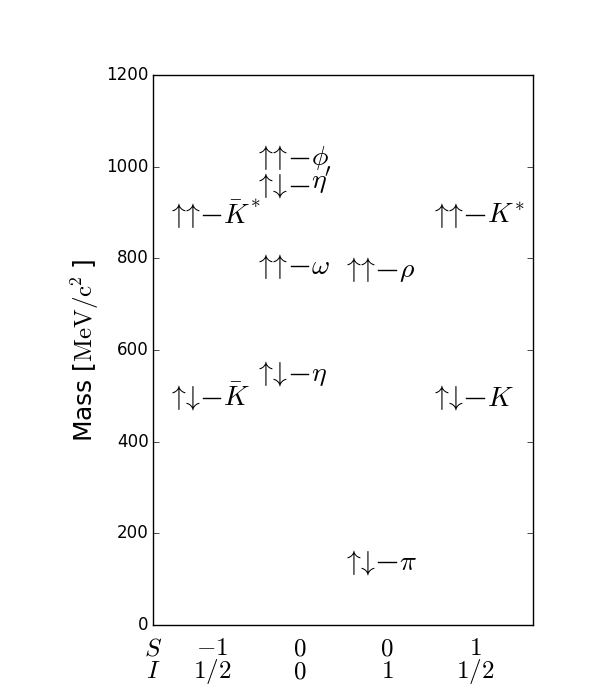
\includegraphics[scale=0.5]{images/meson.png}
\end{center}
\caption{Masses of the pseudo-scalar ($\uparrow\downarrow$) and vector ($\uparrow\uparrow$) mesons.  }\label{fig:mesonMasses}
\end{figure}
The dynamic mass is essentially the same for all quarks, regardless of the quark flavour. The dynamic part of the mass is important or the light quarks was not very important in the charmonium and bottomium states.   

This very simple model gives a very good agreement with the observed meson spectrum.
%%\keypoint{ The mass splitting between the mesons in the same multiplet is due to the mass difference between the $s$-quarks and the $u$ and $d$ quarks, and to a spin-spin interaction.}
%%\section{Meson decays}
\subsection{Meson decays}
The discussion of the decays of the light quark mesons is similar to that of the decays of the quarkonia.
\subsubsection{Pion decays}
The neutral pion $\pi^0$ is the lightest meson and therefore cannot decay into another meson. Because of its spin $S=0$ it cannot decay through a virtual photon to an electron-positron pair. It decays to two photons.
%%\keypoint{The neutral pion decays into two photons.}
\begin{center}
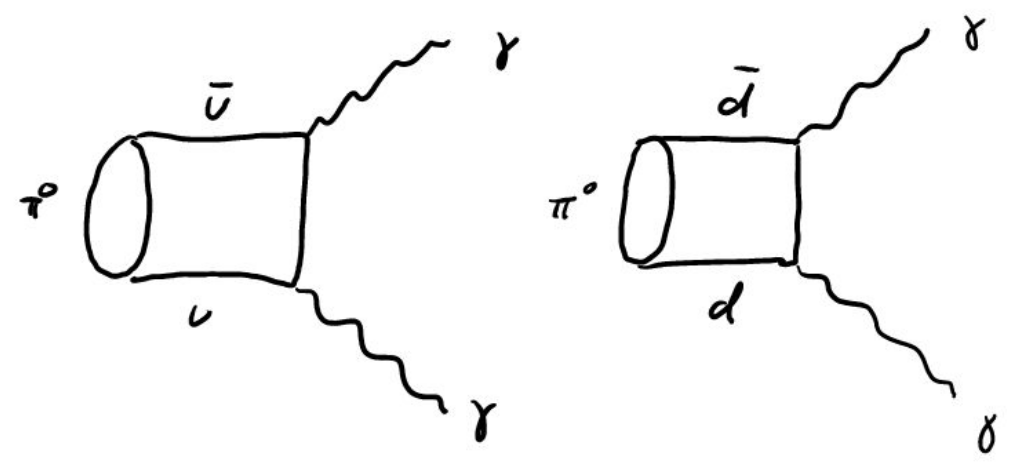
\includegraphics[scale=0.3]{images/pi0Decay.png}
\end{center}
The charged pions $\pi^+,\pi^-$ are the lightest states with quarks of different flavours. The cannot decay through a virtual photon for the same reason as the $\pi^0$ and because of electric charge conservation. The decay to two photons is not allowed, again because of electric charge conservation. The only channel left for them to decay is through the weak interaction: they can annihilate into an off-shell $W$ boson which promptly decays into a charged lepton and a neutrino. From the perspective of the mass the charged lepton can be either an electron or a muon. We will see later that the decay with a muon is preferred. 
\begin{center}
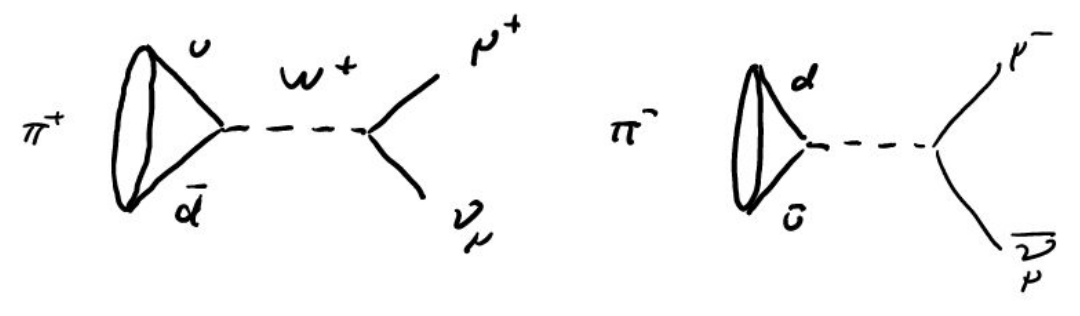
\includegraphics[scale=0.3]{images/piDecay.png}
\end{center}
Due to the fact that it can only decay through the weak interaction the charged pions have a much longer lifetime than the neutral pions.
%%\keypoint{The charged pions decay weakly and have therefore a much longer lifetime than the neutral pions.}
\subsubsection{Kaon decays}
The kaons are mesons with one $s$ quark or $\bar s$ antiquark. For the neutral kaons $K^0$ and $\bar K^0$  the $s$ quark has to decay through the weak interaction into a $u$ quark. 
\begin{center}
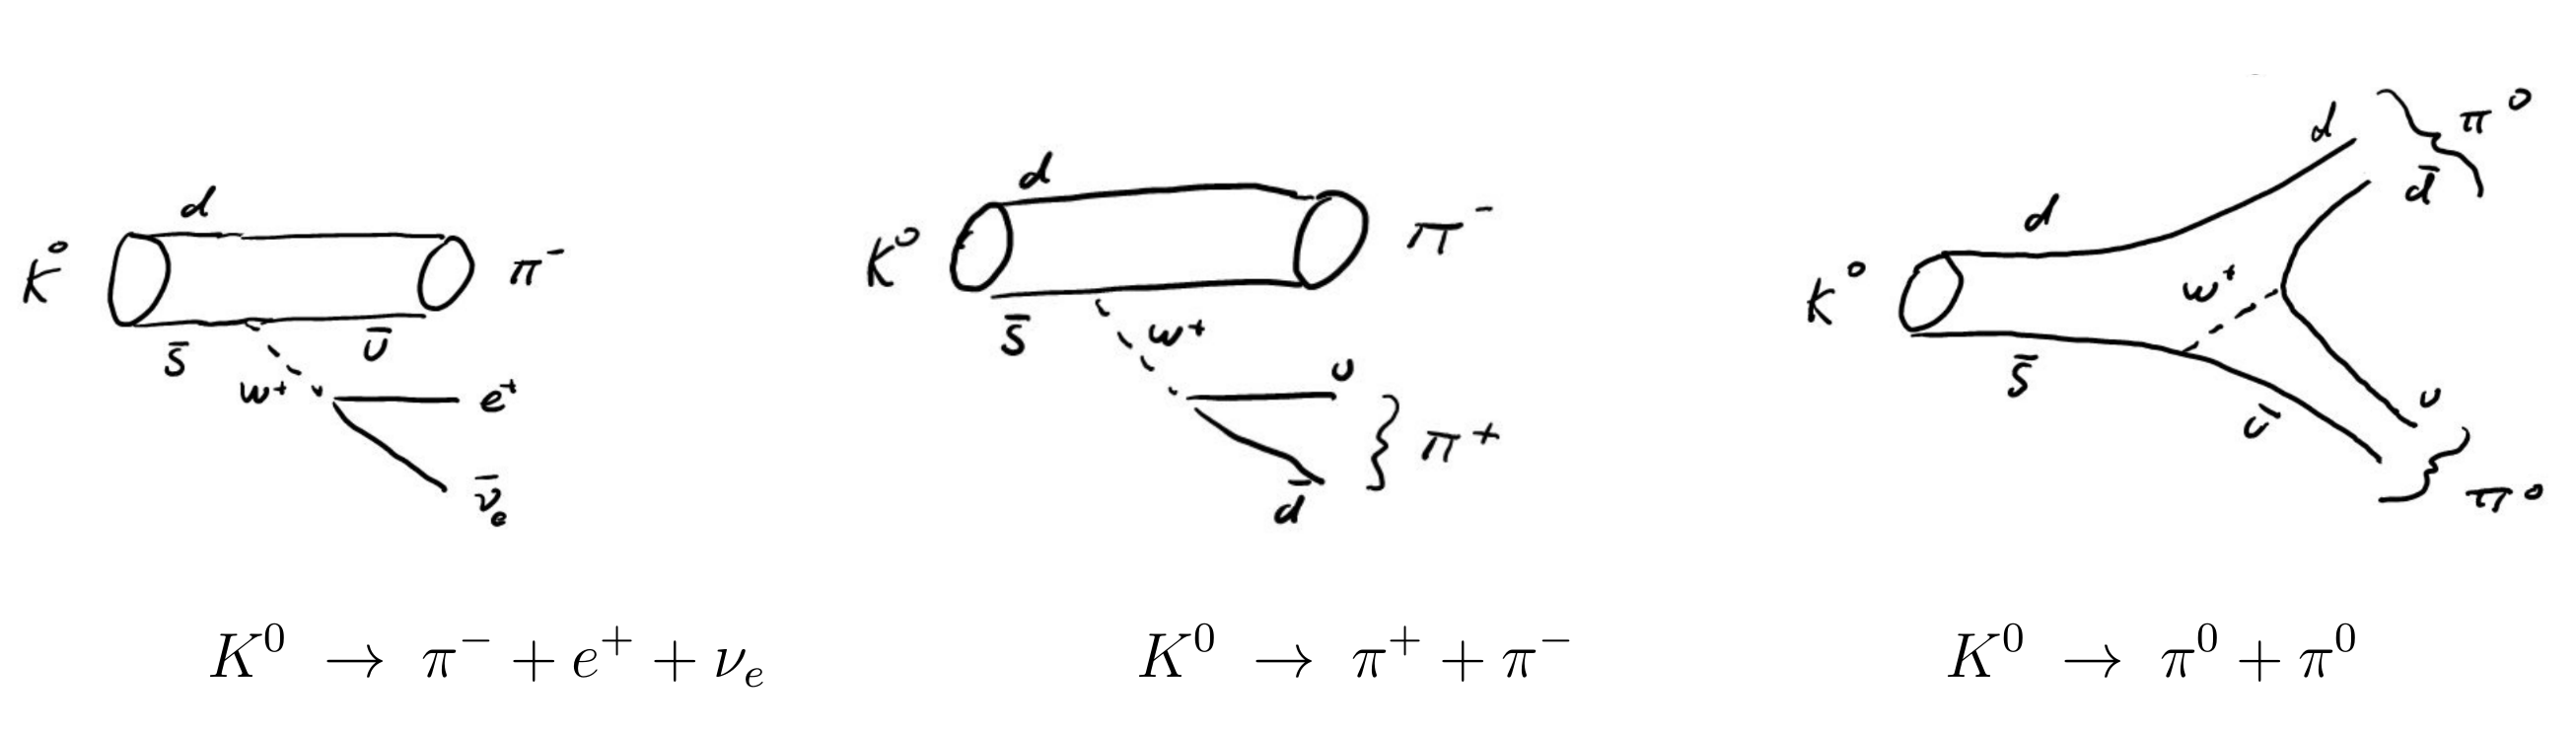
\includegraphics[scale=0.15]{images/k0decay.png}
\end{center}
Because of the heavier mass of the kaons it is also kinematically possible for them to decay into three pions.
%%\image{K0Decay3.png}
\begin{center}
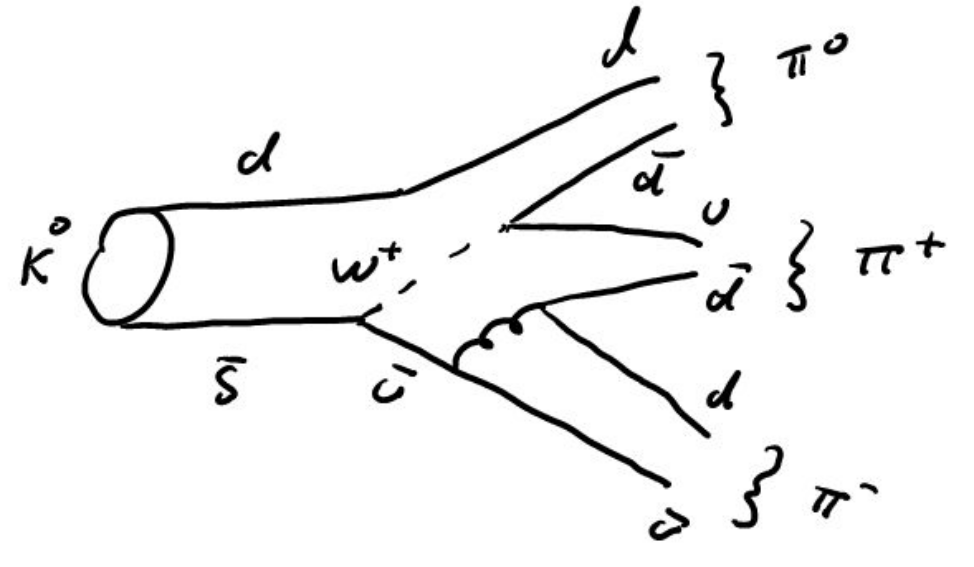
\includegraphics[scale=0.2]{images/K0Decay3.png}
\[
K^0\;\rightarrow\; \pi^+ +\pi^-+\pi^0
\]
\end{center}
For the charged kaons $K^+$ and $K^-$ the same decay is possible and the two quarks can annihilate into an off-shell $W$ boson as in the case of the charged pions.  
%%\keypoint{The scalar kaons can only decay weakly and has therefore a long lifetime}
\begin{center}
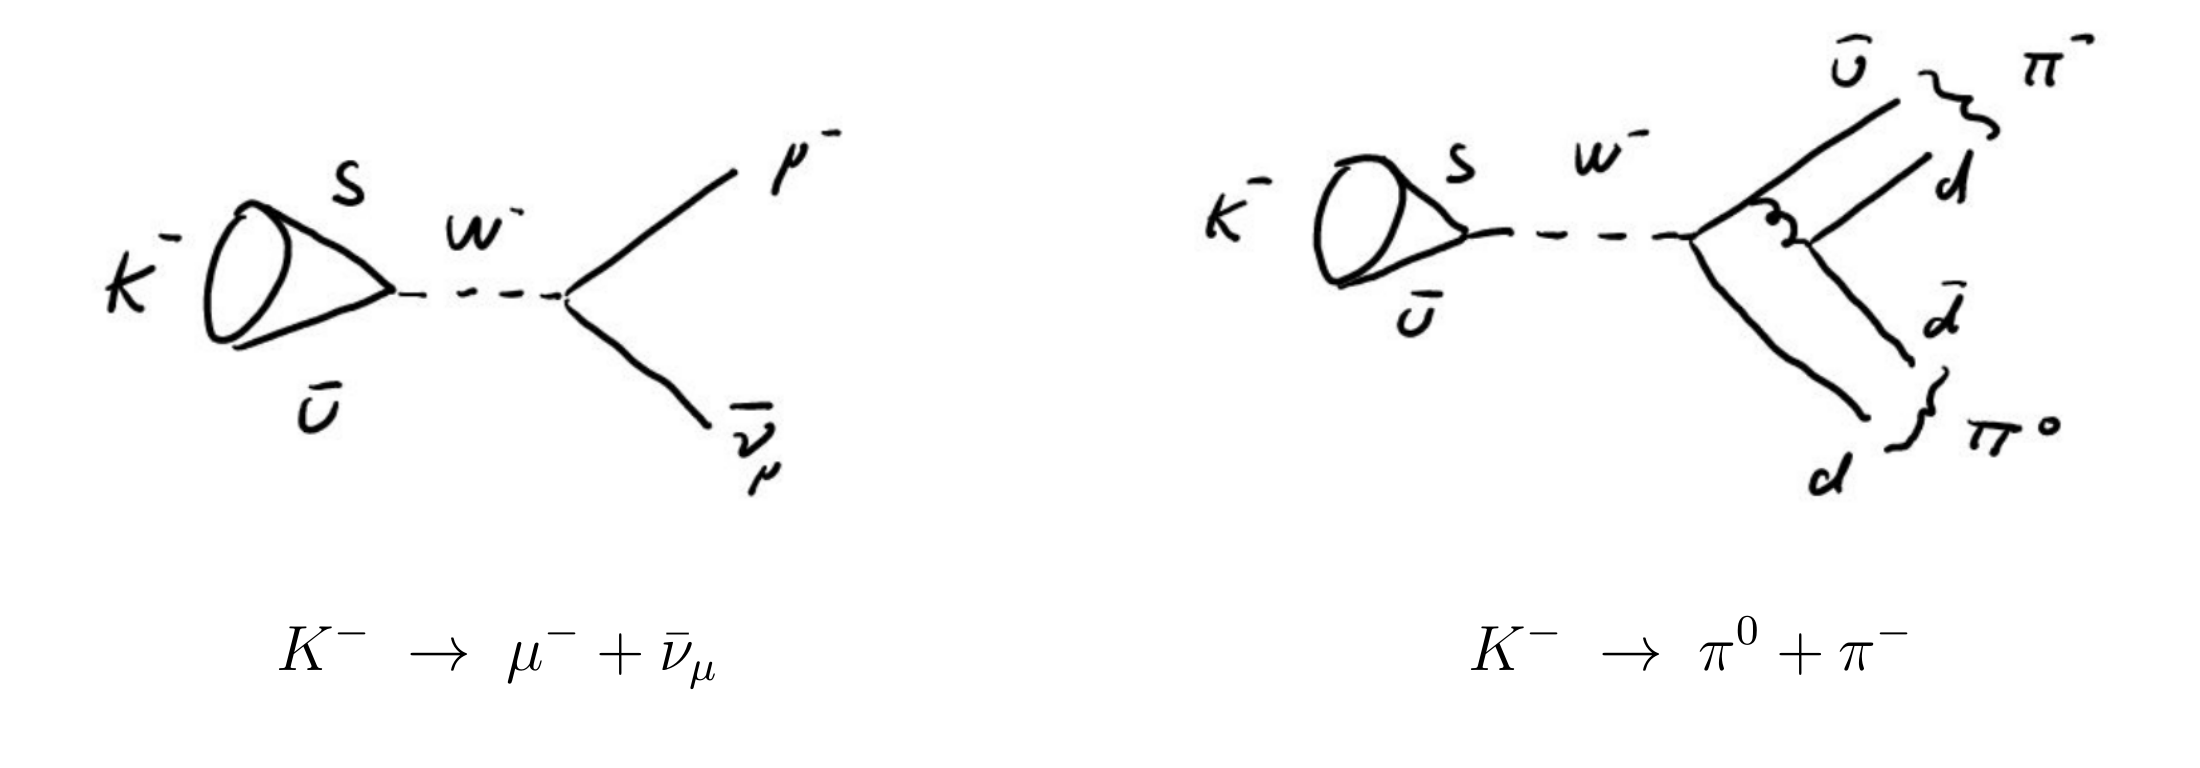
\includegraphics[scale=0.25]{images/kaonWeak.png}
\end{center}
\subsubsection{Vector mesons}
Because the mass difference between the vector mesons mass and their corresponding pseudo-scalar meson is larger than the pion mass, the vector meson can decay through the strong force into pseudo-scalar mesons. Because this decay is mediated through the strong force it is much more likely than other decay mode involving the electro-magnetic or weak force. 
%%\keypoint{The vector mesons decay into their pseudo-scalar counterparts and pions.}
\begin{center}
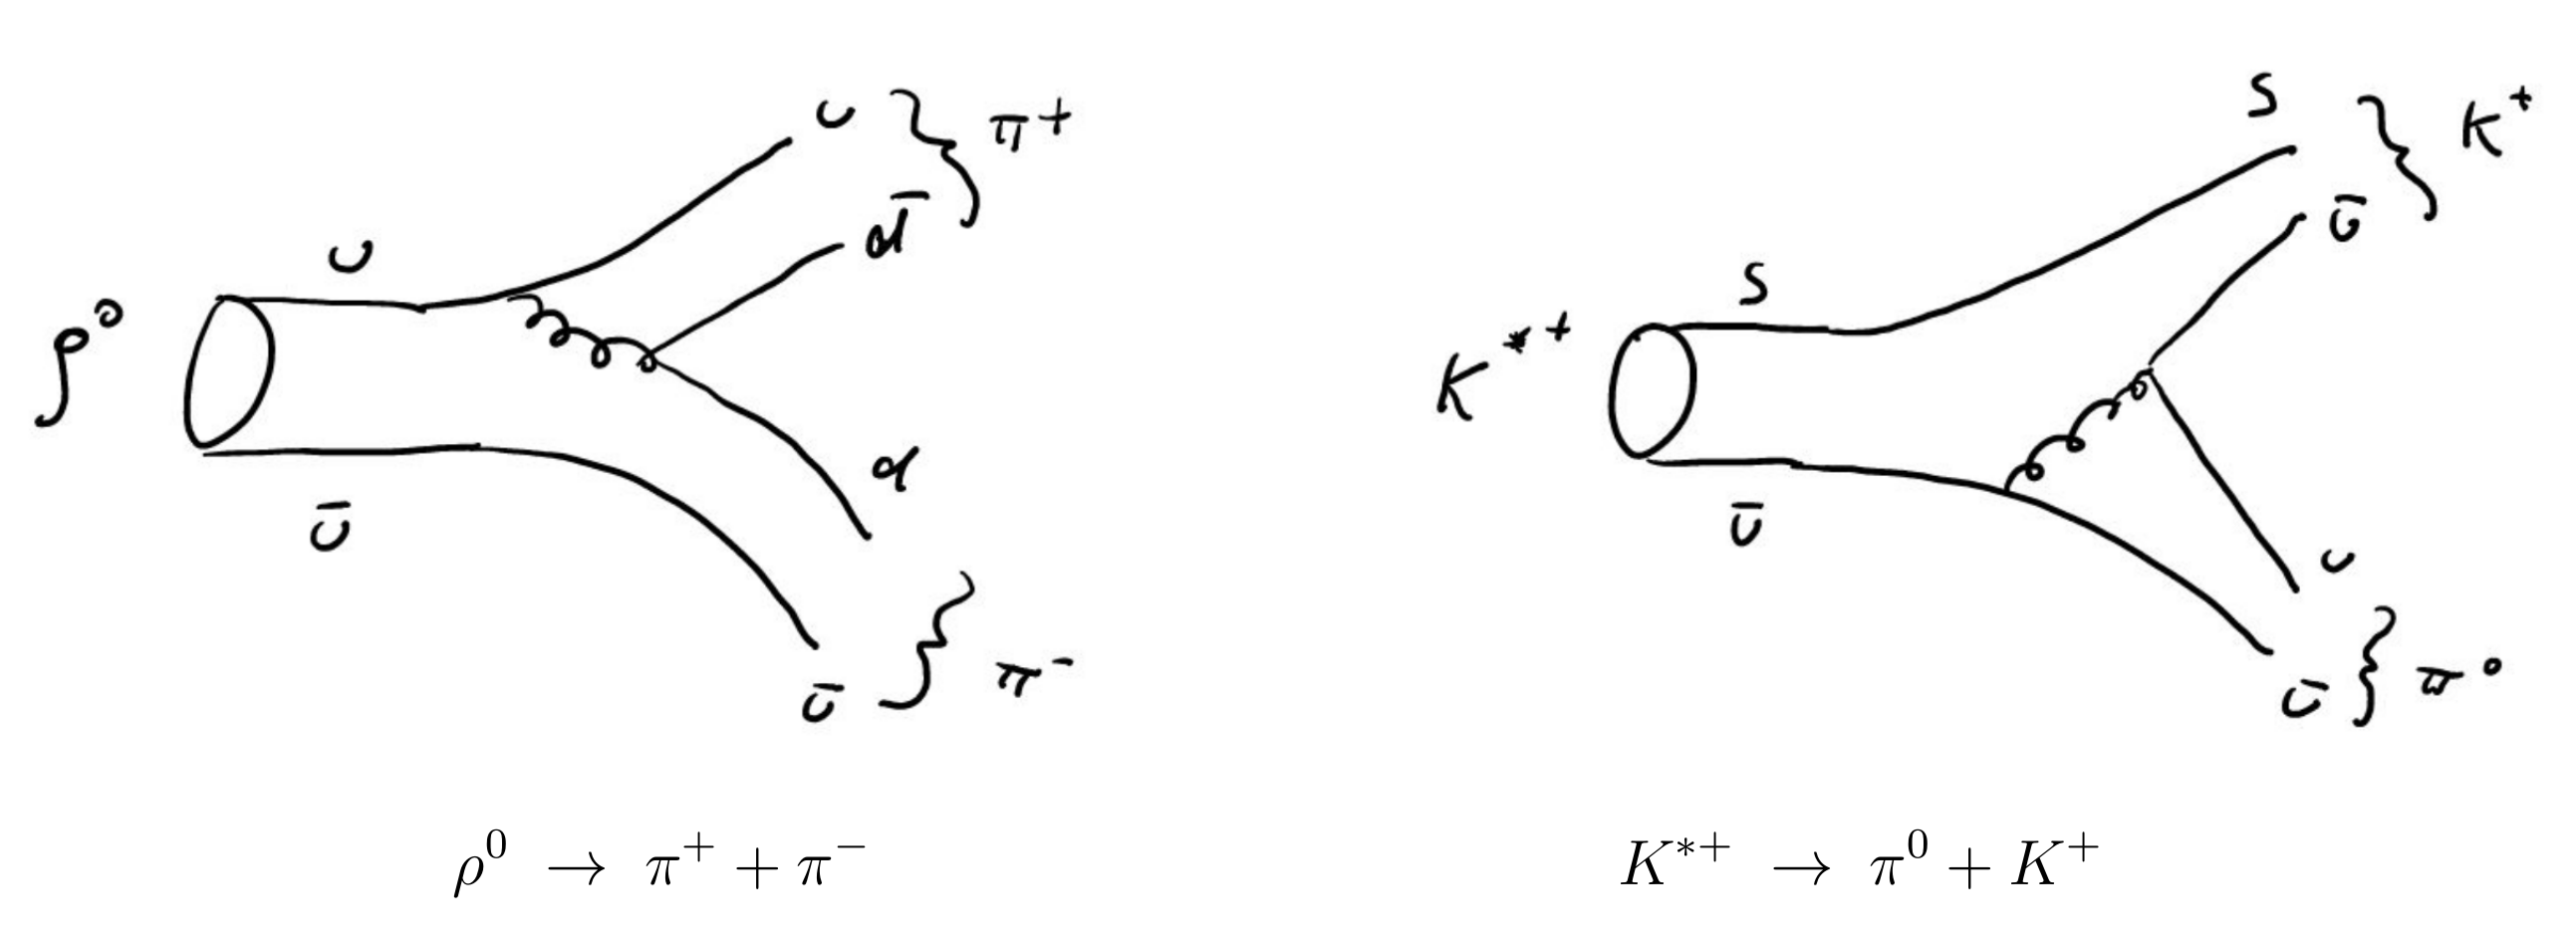
\includegraphics[scale=0.2]{images/vectorMesonsDecay.png}
\end{center}
   
Table~\ref{tbl:mesonDecay} shows the measured masses of the mesons and their most important decay channels. 
\begin{table}
\begin{center}
\begin{tabular}{|ccc|cc|c|c|}
\hline
 & $J^P$ & I & \multicolumn{2}{c|}{Mass [${\rm MeV/c^2}$]} & $\tau$/s & Decays\\
&&& Calc. & Measured& &\\
\hline
$\pi$ & $0^-$ & $1$ & $140$ & $\pi^0\ \ \ \ 134.98\!\!\! $   &$8.5\times10^{-17}$ & $\pi^0\to\gamma\gamma$~99\%\\
      &       &     &       & $\pi^\pm\ \ \ \ 139.57\!\!\! $ &$2.6\times10^{-8}$  & $\pi^+\to\mu^+\nu_\mu$~100\% \\
 $K$ &$0^-$ & $\frac12$ & $485$ & $K^0_S\ \ \ \ 497.61$ & $8.9\times10^{-11} $ & $K^0_S\to\pi\pi$~100\%\\
     &      &           &       & $K^0_L\ \ \ \ 497.61$   & $5.1\times10^{-8}$ & $K^0_L\to3\pi$~34\%\\
     &      &           &       &   & & $K^0_L\to\pi\mu\nu$~27\%\\
     &      &           &       &   & & $K^0_L\to\pi e\nu$~39\%\\
     &      &           &       & $K^+\ \ \ \ 493.68$ & $1.2\times10^{-8}$ & $K^+\to\mu^+\nu_\mu$~64\% \\
     &      &           &       &                     &                   & $K^+\to\pi^+\pi^0$~21\%\\
     &      &           &       &                     &                   & $K^+\to\pi\pi\pi$~7\%\\
$\eta$  &  $0^-$ &$0$& $559$ & $547.853$& $5.1\times10^{-19}$ &$\eta\to3\pi$~55\%\\
        &        &   &       &          & &$\eta\to\gamma\gamma$~39\%\\
$\eta'$ &  $0^-$ &$0$& -- & $957.78$&$3.3\times10^{-21}$& $\eta'\to\pi\pi\eta$~65\%\\
        &        &   &       &       &   & $\eta'\to\rho^0\gamma$~30\%\\
\hline
$\rho$ & $1^-$ & $1$ & $780$ & $775.5$& $4.4\times10^{-24}$ & $\rho\to\pi\pi$~100\%\\
$K^*$ &$1^-$ & $\frac12$ & $896$ & $\begin{array}{cc}895.94 & K^{*0}\\ 891.66 & K^{*+}\end{array}\!\!\!\!\!\!$ & $1.3\times10^{-23}$ & $K^*\to K\pi$~100\%\\
$\omega$ & $1^-$ & $0$ & 780 &$782.65$& $7.8\times10^{-23}$ & $\omega\to\pi^0\pi^+\pi^-$~89\%\\
$\phi$ & $1^-$ & $0$ & 1032 & $1019.46$& $1.5\times10^{-22}$ &$\phi\to K\bar{K}$~83\%\\
         &        &   &       &          && $\phi\to\rho\pi$~13\%\\
\hline
\end{tabular}
\end{center}
\caption{Mass and main decay channels for the mesons formed from light quarks.}\label{tbl:mesonDecay}
\end{table}

\subsection{Additional quarks}
We can imagine extending the description to include the charm quark and argue that these four quarks for a $SU(4)$ multiplet and use this (quite) approximate symmetry to classify mesons build from these four quarks and corresponding antiquarks. While this is possible the patterns expected from the symmetry are less evident because the symmetry is more badly broken, so it is not used much in practice. Appendix~\ref{sec:Symmetries} shows plots of charmed mesons classified according to multiplets of the $SU(4)$ symmetry. 
\clearpage
%%\lecture{21}
%%\section{Baryons}
\section{Baryons}
%%
%%
Baryons are bound states of three quarks or three antiquarks. Protons and neutrons are examples of baryons. We will only consider the baryons with quarks, a similar discussion applies to the antiquark bound state. We consider baryons containing $u$, $d$ and $s$ quarks. We only consider the ground states of these bound states with $L=0$.
%%\keypoint{Baryons are bound states of three quarks. Anti-baryons are bound states of three anti-quarks.}

Both for the spin and the isospin of the bound state we need to consider the combination of three spin/isospin $1/2$ particles: \[{\bf \frac{1}{2}}\otimes{\bf \frac{1}{2}}\otimes{\bf \frac{1}{2}}
=
{\bf \frac{1}{2}}\oplus{\bf \frac{1}{2}}\oplus{\bf \frac{3}{2}}\]
Since the three quarks in the baryon have spin $1/2$ the baryons can have either spin $1/2$ or spin $3/2$ (see appendix~\ref{sec:Symmetries}). The baryons can also be classified by their isospin. If a baryon contains no $u$ or $d$ quark then it is an isospin singlet. If it contains only one $u$ or one $d$ quark it is part of an isospin doublet. If there are two $u$ or $d$ quarks the can either form an isospin $I=1$ triplet or an isospin $I=0$ singlet. Finally if there are three $u$ and $d$ quarks they can either form an isospin $I=3/2$ quartet or an isospin $I=1/2$ doublet. These results are collected in Table~\ref{tbl:baryons}
%%\keypoint{There are baryons with spin $1/2$ and baryons with spin $3/2$.}
\begin{table}
\begin{center}
\begin{tabular}{|c|c|c|}
\hline
\# s-quarks, Strangeness  & isospin  &  baryons \\\hline
0 ($S=0$)  & ${\bf \frac{1}{2}}\otimes{\bf \frac{1}{2}}\otimes{\bf \frac{1}{2}}
=
{\bf \frac{1}{2}}\oplus{\bf \frac{1}{2}}\oplus{\bf \frac{3}{2}}$   & \\
  & $I=3/2$   & $\Delta$ baryons \\
    & $I=1/2$   & Nucleons $n$, $p$\\\hline
1 ($S=-1$)  & ${\bf \frac{1}{2}}\otimes{\bf \frac{1}{2}}
=
{\bf 1}\oplus{\bf 0 }$  & \\
& $I=1$ &  $\Sigma$\\
& $I=0$ &  $\Lambda$\\\hline
2 $S=-2$ & $I=1/2$ & $\Xi$ \\\hline
3 $S=-3$ & $I=0$ & $\Omega$\\\hline
\end{tabular}
\end{center}\caption{Baryons with $u$, $d$ and $s$ quarks with their isospin and strangeness.}\label{tbl:baryons}
\end{table}  
\subsection{Baryon wave-function}
Unlike in the mesons where we had a quark and an anti-quark, in the baryons we have only quarks so we have the possibility of having identical quarks in the bound state. The wave function for identical fermions has to satisfy the Pauli exclusion principle: it has to be anti-symmetric with respect to the exchange of any two identical particles. The total wave-function is the (tensor) product of the spatial, flavour, spin and colour wave functions.
\[\psi_{\rm total}
=
\psi_{\rm spatial}\cdot
\psi_{\rm flavour}\cdot
\psi_{\rm spin}\cdot
\psi_{\rm colour}
\] 
Since we only consider the lowest state the spatial wave function is symmetric. The colour wave function is totally anti-symmetric. There are several ways of explaining this fact. One physical reason is that the $\Delta^{++}$ resonance has three valence $u$ quarks and spin $3/2$, therefore (assuming the lowest state for the spatial wave function) we have symmetric spatial, spin and flavour wave function, the last chance for the total wave function to be anti-symmetric is to have a totally anti-symmetric. This reasoning was one of the reasons colour was introduced as an additional quantum number was requested in order to satisfy the Pauli exclusion principle. Another explanation is more mathematical: if we look at the transformation behaviour of a combination of three triplets we get:
\[\bf 3 \otimes 3 \otimes 3 = 10\oplus 8 \oplus 8\oplus 1\;,\]
that is we get a decuplet, two octets and a singlet. The singlet is the combination we are interested in because we want the baryon to be colour neutral. An explicit calculation (see python server) shows that the combination corresponding to the singlet is totally anti-symmetric:
\[\psi_{\rm colour}=\frac{1}{\sqrt{6}}\left(
\left|rgb\right>
-\left|rbg\right>
+\left|brg\right>
-\left|bgr\right>
+\left|gbr\right>
-\left|grb\right>
\right)\;.\]   
With the symmetric spatial and the anti-symmetric colour wave function we need the combination of the spin and flavour wave function to be symmetric for identical particles. While at this stage we only need to impose this condition for quarks of the same flavour we will impose it to all quarks, regardless of the flavour and we will see that agrees with the observed baryon states. We can now work out the consequence of the Pauli exclusion principle for the spin and flavour wave function of the baryons. We will treat three cases.
\begin{description}
\item[all three quarks are of the same flavour:] in this case we have three identical particles, since the flavour wave function is totally symmetric the spin wave function has to be symmetric. The totally symmetric spin wave function for three spin $1/2$ particles corresponds to the spin $3/2$ combinations. So we know that the baryons with flavour combinations $uuu$, $ddd$ and $sss$ will have spin $3/2$.
\item[two quarks have the same flavour:] these combinations are $uud$, $uus$, $ddu$, $dds$, $ssu$ and $ssd$. For the two identical quarks we have a symmetric flavour wave function so the spin wave function has to be symmetric. For two spin $1/2$ particles the symmetric combination corresponds to spin $1$. This means that within a baryon with two quarks of the same flavour these two quarks have combined spin $1$. (Note that this is true of the baryons with three identical flavour quarks: each pair of quarks is in a spin 1 combination.) If we now add the third quark with the different flavour we can get either a spin $3/2$ or a spin $1/2$ combination.
\item[all three quarks have different flavours:] In the $uds$ state we first consider the $ud$ quarks system. it can be in either a symmetric or anti-symmetric combination:
\begin{itemize}
\item symmetric 
\[\frac{1}{\sqrt2}\left(ud+du\right)\;.\]
This corresponds to an isospin $I=1$. Since the flavour wave function is symmetric the spin wave function of the two quarks also has to be symmetric, that is the spin of the $ud$ pair is $S=1$. If we add the $s$ quark we can get either a spin $3/2$ or a spin $1/2$ combination.
\item anti-symmetric 
\[\frac{1}{\sqrt2}\left(ud-du\right)\;.\]
This corresponds to an isospin $I=0$. Since the flavour wave function is anti-symmetric the spin wave function of the two quarks also has to be anti-symmetric, that is the spin of the $ud$ pair is $S=0$. If we add the $s$ quark we can only get a spin $1/2$ combination.
\end{itemize}
So we expect three different $uds$ states: one with spin $3/2$ and two with spin $1/2$, differing by whether the $ud$  pair is in a spin $1$ or spin $0$ state.
\end{description}
We start with the spin $3/2$ states, they have a fully symmetric flavour wave function. In the decomposition 
\[\bf 3\otimes 3 \otimes 3 = 10\oplus 8 \oplus 8\oplus 1\]
this corresponds to the decuplet. We can arrange the ten $J=3/2$ baryons in the same plane with the third component of the isospin in the $x$ direction and the strangeness in the $y$ direction, as depicted in figure~\ref{fig:baryonDecuplet}. 
%%\image{BaryonDecuplet.png}
\begin{figure}
\begin{center}
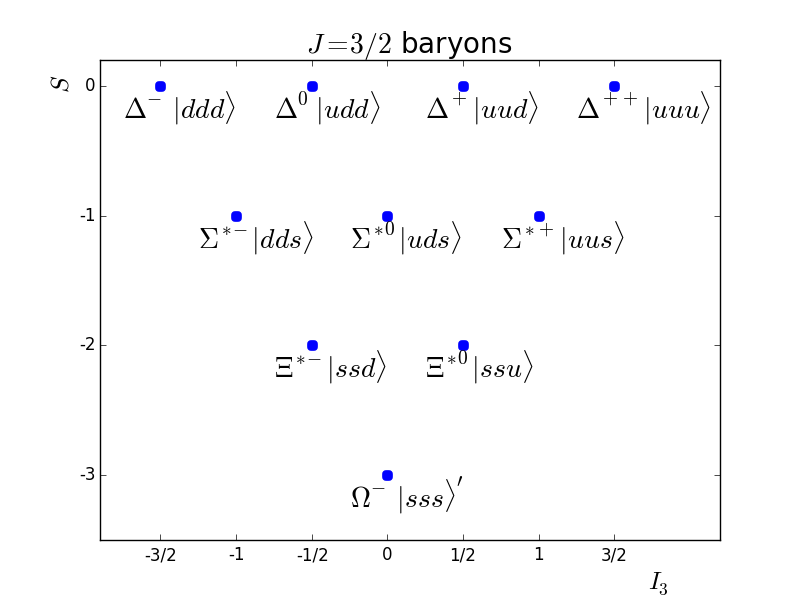
\includegraphics[scale=0.5]{images/BaryonDecuplet.png}
\end{center}
\caption{Baryon decuplet in the plane of the third component of the isospin and strangeness plane. The symmetrisation over the flavours is implied, for example $|uud\rangle$ stands for $(
|uud\rangle+|udu\rangle+|duu\rangle)/\sqrt3$. }\label{fig:baryonDecuplet}
\end{figure}
Each row in figure~\ref{fig:baryonDecuplet} is an isospin multiplet: the $\Delta^{-,0,+,++}$ baryons form an isospin $I=3/2$ quadruplet, the $\Sigma^{*-,0,+}$ baryons form an isospin $I=1$ triplet, the $\Xi^{*-,0}$ baryons form an isospin $I=1/2$ doublet and the $\Omega^-$ baryon is an isospin singlet.  

For the spin $1/2$ baryons the spin wave function is neither totally symmetric not totally anti-symmetric, so in order to obtain a symmetric spin-flavour wave function (in order to have an anti-symmetric total wave function) we need to combine the the mixed-symmetry spin wave function with mixed-symmetry flavour wave functions. in the decomposition 
\[\bf 3\otimes 3 \otimes 3 = 10\oplus 8 \oplus 8\oplus 1\] 
the two octets correspond to different mixed symmetries of the flavour wave function. The derivation of the exact wave function is somewhat tedious but the main result but the symmetry consideration is enough to conclude that the spin $1/2$ baryons have to be in a flavour octet. Figure~\ref{fig:baryonOctet} shows this octet. 
\begin{figure}[h]
\begin{center}
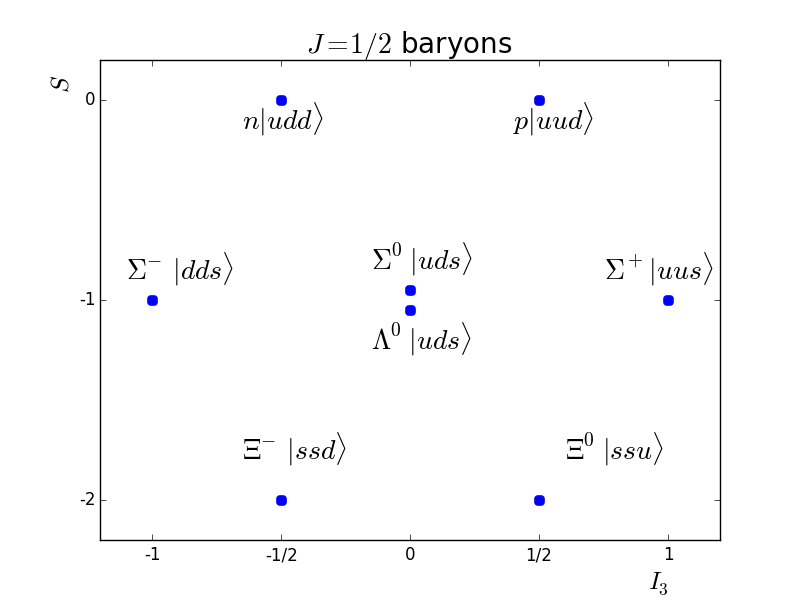
\includegraphics[scale=0.5]{images/BaryonOctet.png}
\end{center}
\caption{Baryon decuplet in the plane of the third component of the isospin and strangeness plane.}\label{fig:baryonOctet}
\end{figure}
We are left with the flavour singlet to discuss. The $SU(3)$ flavour singlet is totally anti-symmetric (we saw this for when we discussed the colour wave function) so we would need the spin wave function to be totally anti-symmetric, but in the combination of 3 spin $1/2$ particles we have a totally symmetric combination (spin 3/2) and two mixed symmetry spin $1/2$ multiplets, but no combination that is totally anti-symmetric. So we do not have a way of satisfying the Pauli exclusion principle and there is no state that corresponds to the flavour singlet.
%%\keypoint{ Depending on the number of $s$-quarks in them, the baryons form different isospin multiplets.}
%%\keypoint{The condition that the wave function of the quarks in the baryon satisfies the Pauli principle imposes constraints on what spins and isospin combination are possible.}
%%
%%
\subsection{Baryon masses}
%%
%%
\begin{wrapfigure}{r}{0.4\textwidth}
\begin{center}
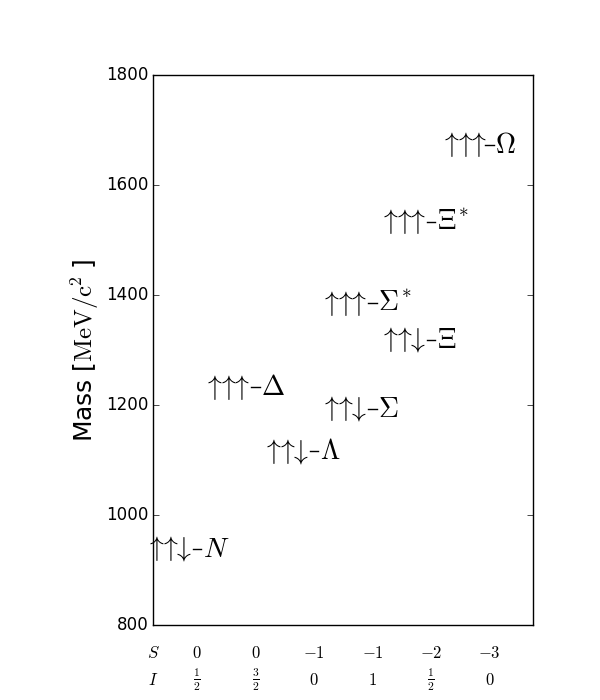
\includegraphics[scale=0.5,trim=7cm 1cm 5cm 5cm]{images/baryon.png}
\end{center}
\caption{Spectrum of the baryons made of light quarks.}\label{fig:baryonSpectrum}
\end{wrapfigure}
Looking at the baryon spectrum in figure~\ref{fig:baryonSpectrum} we see that $J=3/2$ states are heavier than $J=1/2$ states, we also notice that the mass increases as the number of $s$ quarks increases. 

As for the mesons the mass difference can be traced to the spin-spin interaction between the valence quarks. The interaction is given by
\[V_{ss}(q_i,q_j)=\frac{16\pi}{9}\alpha_s\frac{\vec s_i\cdot \vec s_j}{m_i m_j}\delta(\vec x)\;.\]
The prefactor is different because the colour charges combination is different in a $qq$ pair than in a $q\bar q$ pair. Now for the baryons we have three quarks so we need to sum over all the quark pairs. For the nucleons, $\Delta$ baryons and the $\Omega$ baryon we can use
\[\vec J^2=(\vec s_1 +\vec s_2+\vec s_3)^2=3\frac{3}{4}+2\sum\limits_{i<j}\vec s_i\cdot \vec s_j\]
\begin{eqnarray*}
\Rightarrow&& \sum\limits_{i<j}\vec s_i\cdot\vec s_j=\frac{1}{2}\left(J(J+1)-\frac{9}{4}\right)
=\left\{\begin{array}{ccc}
\displaystyle\frac{3}{4}&\mbox{for}& J=3/2\\\\
\displaystyle-\frac{3}{4}&\mbox{for}& J=1/2\\
\end{array}\right.
\end{eqnarray*}
so we get a contribution 
\[E_{ss}=\left\{
\begin{array}{cc}
-\displaystyle\frac34\frac{16\pi}{9}\frac{\alpha_s}{m_{u,d}^2}|\psi(0)|^2&\mbox{for nucleons}\\
\displaystyle\frac34\frac{16\pi}{9}\frac{\alpha_s}{m_{u,d}^2}|\psi(0)|^2&\mbox{for $\Delta$ baryons}\\
\displaystyle\frac34\frac{16\pi}{9}\frac{\alpha_s}{m_s^2}|\psi(0)|^2&\mbox{for the $\Omega$ baryon.}
\end{array}
\right.\]
where we have assumed that the $u$ and $d$ quark have the same mass $m_u=m_d=m_{u,d}$.

The situation is more complicated when the quark masses are not the same, since then needs to know the relative spins of the quarks within the bound state. We have seen earlier with the quarkonia that for a pair of spins we have 
\[\langle \vec s_1 \cdot\vec s_2 \rangle=\frac{2S(S+1)-3}{4}=\left\{\begin{array}{ccc}-\frac{3}{4}&\mbox{for}& S=0 \\ +\frac{1}{4}&\mbox{for}& S=1 \end{array}\right.\] 

We take as an example the $uds$ baryons. First we look at the $J=3/2$ state. This state has a totally symmetric spin wave function, so any two spins are in a symmetric combination, meaning that they are in a spin $1$ combination. So we get for each pair the same factor of $+1/4$ for $\langle \vec s_i\cdot \vec s_j\rangle $, the only difference between the pair is the product of masses in the denominator. We get for the spin $3/2$ state:
\[E_{ss}^{\Sigma^{*0}}
=
\displaystyle\frac{16\pi\alpha_s}{9}\frac{1}{4}\left(
\frac{1}{m_u m_d}
+
\frac{1}{m_u m_s}
+
\frac{1}{m_d m_s}
\right)|\psi(0)|^2
\]  
For the $J=1/2$ baryons the situation is more complicated. We have two cases: for the $\Sigma^0$ particle has isospin $1$ and therefore the $u$ and $d$ quarks combine in a spin $1$ state. so we have 
\[\left<\vec s_u \cdot \vec s_d\right>=+\frac14\;,
\qquad J(J+1)=\frac{9}{4}
+2 \vec s_u\cdot \vec s_d
+2 \vec s_u\cdot \vec s_s
+2 \vec s_d\cdot \vec s_s
=\frac{11}{4}+2 \vec s_u\cdot \vec s_s
+2 \vec s_d\cdot \vec s_s
\]
The $s$-quark is not in a combination with a definite spin with the $u$ or $d$ quark, so we have
\[E_{ss}^{\Sigma^{0}}
=
\displaystyle\frac{16\pi\alpha_s}{9}\left(
\frac{1/4}{m_u m_d}
+
\frac{\left<\vec s_u\cdot \vec s_s\right>}{m_u m_s}
+
\frac{\left<\vec s_d\cdot \vec s_s\right>}{m_d m_s}
\right)|\psi(0)|^2
\]  
If we assume $u$ and $d$ masses are the same we can calculate the last two fractions and the contribution to the mass
\[\vec s_u\cdot \vec s_s
+\vec s_d\cdot \vec s_s=\frac{1}{2}\left(\frac34-\frac{11}{4}\right)=-1
\]
\[E_{ss}^{\Sigma^{0}}
=
\displaystyle\frac{16\pi\alpha_s}{9}\frac14\left(
\frac{1}{m_{u,d}^2}
-
\frac{4}{m_{u,d} m_s}
\right)|\psi(0)|^2\;.
\]  
The reasoning is the same for the $\Lambda^0$ baryon except that the expectation value of $\vec s_u\cdot \vec s_d$ is $-3/4$. We get
\[\left<\vec s_u \cdot \vec s_d\right>=-\frac34\;,
\qquad J(J+1)=\frac{9}{4}
+2 \vec s_u\cdot \vec s_d
+2 \vec s_u\cdot \vec s_s
+2 \vec s_d\cdot \vec s_s
=\frac{3}{4}+2 \vec s_u\cdot \vec s_s
+2 \vec s_d\cdot \vec s_s
\]
\[\Rightarrow\vec s_u\cdot \vec s_s
+\vec s_d\cdot \vec s_s=\frac{1}{2}\left(\frac34-\frac{3}{4}\right)=0\;, \]
which give a contribution to the $\Lambda^0$ mass of
\[E_{ss}^{\Lambda^{0}}
=
\displaystyle\frac{16\pi\alpha_s}{9}\left(
-\frac34\frac{1}{m_{u,d}^2}
\right)|\psi(0)|^2\;.
\]  
%%\keypoint{The mass splitting between the $J=3/2$ and $J=1/2$ states can be explained by a spin-spin interaction as in the meson. The form of the interaction depends on the relative spin of the valence quarks. Information about the relative spin can be inferred from symmetry properties of the wave-function.}

As for the mesons, the mass of the baryons is fairly well described by the constituent mass of the quarks and the contribution from the spin-spin interaction. It is worth noting here that the constituent mass of the quarks in the baryons is different than that in the meson.
%%\keypoint{The constituent mass of the quarks in the baryon are larger than in the meson.}
This is due to the fact that the "medium" inside a meson is different to that inside a baryon and hence the contribution form the interaction is different. 

\clearpage
%%\lecture{22}
%%\section{Electron-positron collisions}
\section{$e^+e^-$ collisions}
So far we have encountered scattering experiments where a beam of projectile is scattered off a target. A different experimental design is used often in particle physics: instead of colliding a beam and a target one can collide two beams of particles. In an electron-positron collider a beam of electron collides with a beam of electrons. At the intersection of the two beams a detector is placed. There are two typical design for such an experiment, sketched in figure~\ref{fig:colliders}. In a linear collider the two beams are accelerated towards each other and collide at the detector location. In the circular design the two beams circulate in opposite direction and are focused to intersect at the location of the detector. The advantage of the circular design is that beams can be reused to produce may collisions while the beams in a linear collider are lost. An advantage common to both design is that the initial state is very well defined, one can choose the electron and positron energy very precisely. This is to be compared with a DIS experiment where the projectile energy can be chosen but the momentum fraction of the parton involved in the interaction cannot be chosen and one has to consider the convolution over all possible momentum fractions.   
%%\keypoint{$e^+e^-$ collisions are useful because they are a clean initial state with a well defined centre of mass energy. In proton-electron collisions the centre of mass energy of the electron and proton is defined by the experimental setup but the actual centre of mass energy of the elastic collision between the electron and the constituent is only defined statistically through the parton distribution functions.}
%%\image{LinearCollider.png}
\begin{figure}
\begin{center}
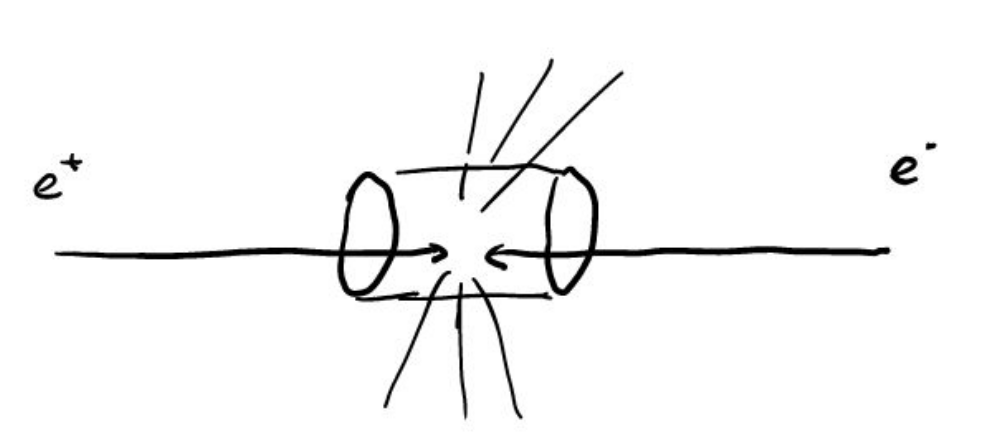
\includegraphics[scale=0.2]{images/LinearCollider.png}
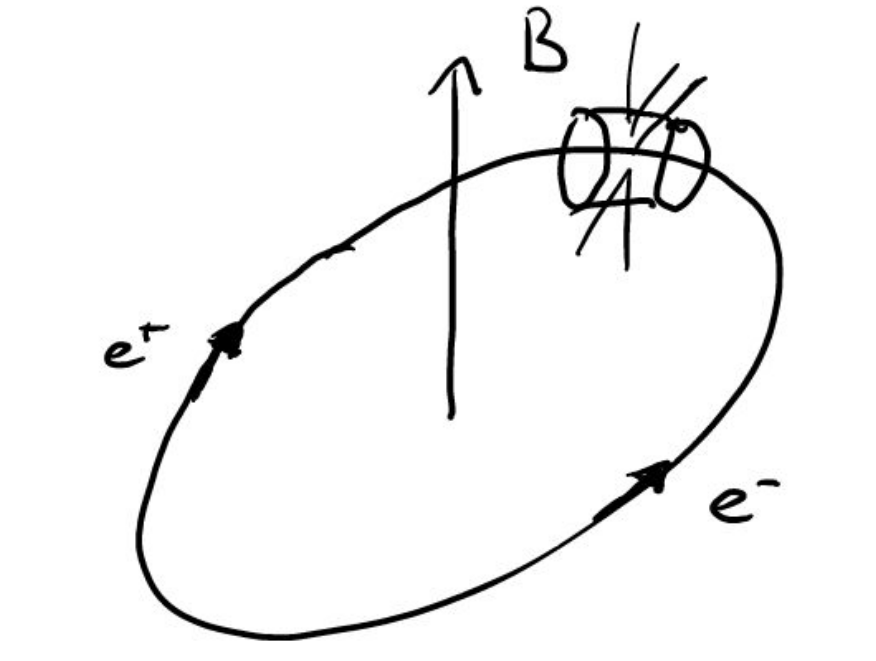
\includegraphics[scale=0.2]{images/CircularCollider.png}
\end{center}
\caption{The two typical collider design: linear collider (left) and circular (right). The beams are kept on a circular trajectory through magnetic fields.}\label{fig:colliders}
\end{figure}
The most important quantity in an $e^+e^-$ collider is the centre of mass energy $s=(p_1+p_2)^2$,
\begin{center}
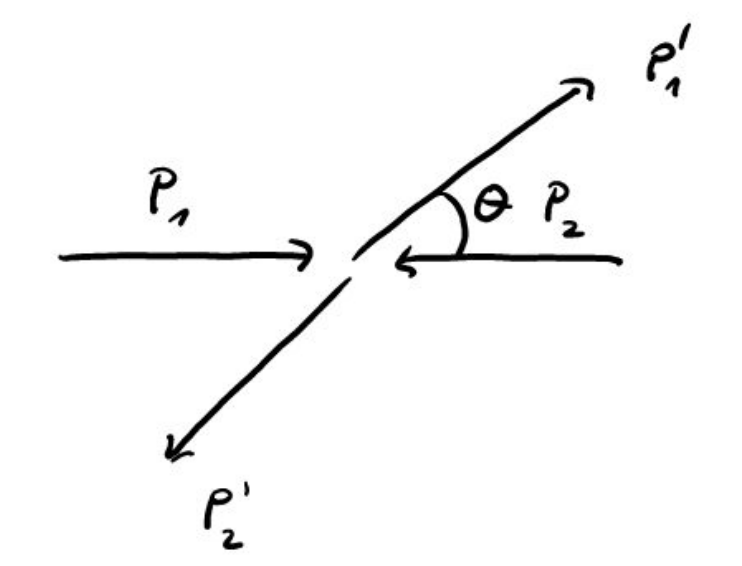
\includegraphics[scale=0.2]{images/epemKinematics.png}
\end{center}
where $p_1$ and $p_2$ are the four-momenta of the electron and positron. $s$ is a Lorentz invariant, its interpretation is easiest in the centre of mass frame (where $\vec p_1=-\vec p_2$):
\[p_1=(E_1,\vec p_1)\;,\quad p_2=(E_2,\vec p_2)\;,\quad s=(p_1+p_2)^2=(E_1+E_2,0)^2=4E^2\;,\]
where we have used the fact that the electron and positron have the same mass, and therefore the same energy in the CMS $E=E_1=E_2$. $\sqrt{s}=2E$ is the total energy available in the collision. If this energy is sufficient we can create new particles. If we want to produce a fermion-antifermion pair with mass $m_f=m_{\bar f}$ we need 
\[\sqrt{s}\geq 2m_f\;.\]
%%
%%
\subsection{Lepton pair production}
%%
%%
The lowest energy process that can happen at an $e^+e^-$ collider is electron scattering. Since the final state particles are already present in the initial state we do not need to "spend" any energy creating them. The possible (lowest order) Feynman diagrams for this process are shown in figure~\ref{fig:epemepem}. 
\begin{figure}
\begin{center}
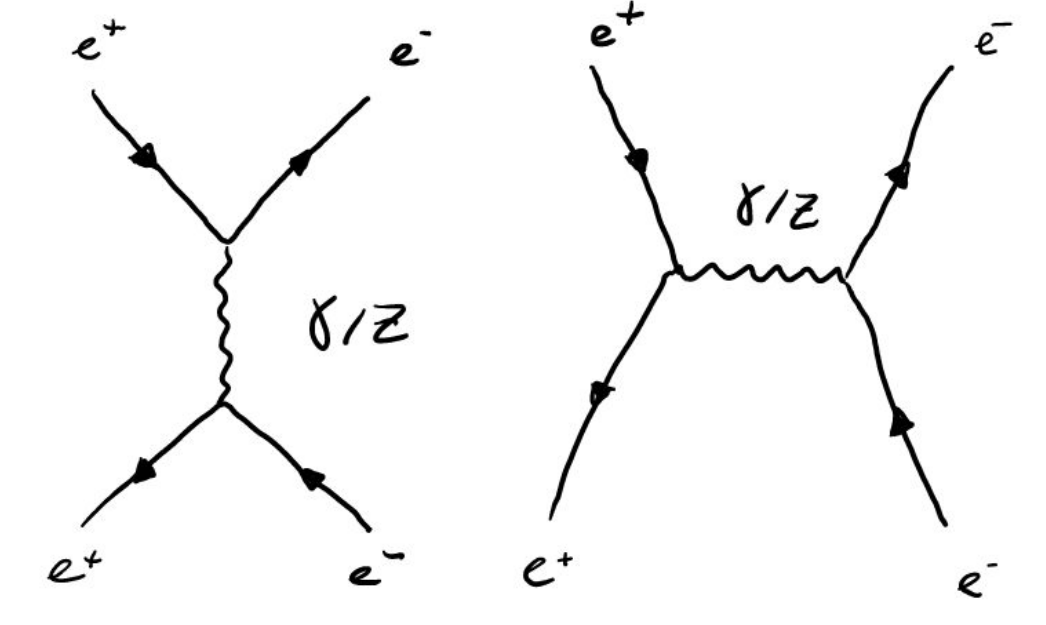
\includegraphics[scale=0.27]{images/epemepem.png}
\end{center}
\caption{Feynman diagrams for the electron-positron scattering. The two possibilities are (left) annihilation into a virtual photon and (right) scattering through exchange of a virtual photon.}\label{fig:epemepem}
\end{figure}
The process can occur through the exchange of a virtual photon, as was the case for the scattering of the electron off the quarks in the DIS process. Since the positron is the antiparticle of the electron there is another possibility: the electron and the positron can annihilate into an off-shell photon and this photon can decay back into an electron-positron pair. Since both processes are allowed the matrix element will be the sum of the two processes and it is not possible to tell whether the one or the other process took place. 

\begin{wrapfigure}{r}{0.5\textwidth}
\begin{center}
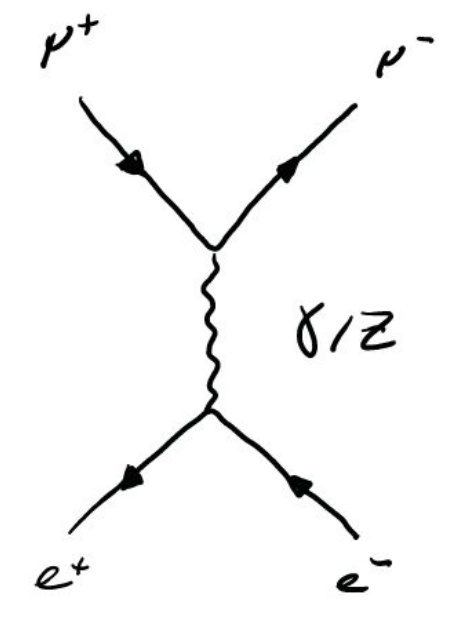
\includegraphics[scale=0.27,trim=0cm 3cm 0cm 5cm]{images/epemmupmum.png}
\end{center}
\caption{Feynman diagram for the muon pair production.}\label{fig:mumu}
\end{wrapfigure}
In both cases where a photon is exchanged a $Z$ boson can also be exchanged but at energies much lower than the $Z$ boson mass $m_Z\simeq 90\,{\rm GeV}$ the contribution for that channel is negligible. 

If the energy is raised particles different to the initial state particles can be produced. The first leptons that can be produced are the muons. The Feynman diagram for this process is shown in figure~\ref{fig:mumu}. This time we only have one Feynman diagram, since we need to annihilate the electron and positron to create the muon pair. The muon has the same quantum numbers as the electron, but its mass is much higher: $m_\mu\simeq 105.7\,{\rm MeV}$. Because its mass is much higher than that of the electron it can decay to an electron (with a muon neutrino and an electron anti-neutrino) through the weak interaction. Since the decay is weak the lifetime of the muon is large, about $2\,{\rm \mu s}$. This means that at the energies at which muons are produced in collider experiments muons have largely time to escape the detector before decaying, which makes them effectively stable for collider experiments. 

\begin{wrapfigure}{l}{0.5\textwidth}
\begin{center}
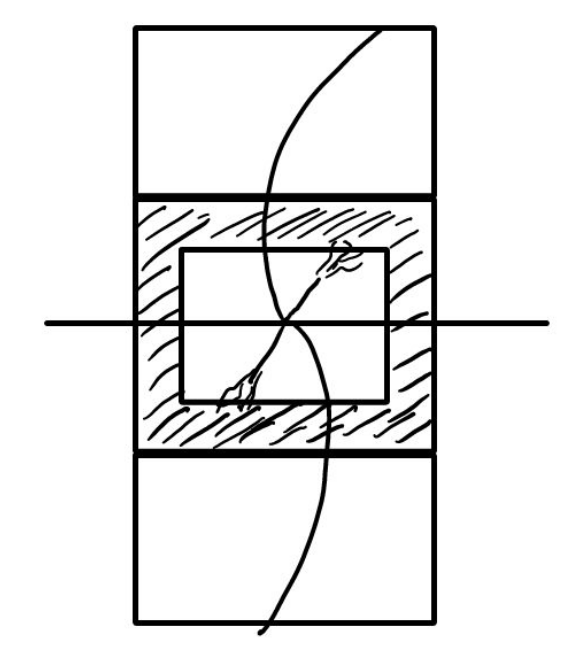
\includegraphics[scale=0.3]{images/electronmuonDetector.png}
\end{center}
\caption{Typical tracks of an electron and muon pair in a particle detector. }\label{fig:electronmuon}
\end{wrapfigure}  	 
Because of their larger mass the muons are not deflected much as they traverse matter, much less than electrons. As they are not deflected much they do not loose much energy and can traverse large distances in any sort of material. This is very different to the electron which loses its energy rapidly in the detector. Experimental tracks of electrons and muons are very different, as sketched in figure~\ref{fig:electronmuon}. The typical detector design has detectors for the electrons close to the collision point and detectors further outside for the muons. Particle detectors typically have strong magnetic fields that allow to identify charged particle by the curvature of their trajectories. Because of these properties the muons are easy to measure and are often used as a reference process. 

If the energy is increased further the heaviest leptons , the $\tau$ leptons can be produced. The $\tau$-lepton mass is $m_\tau\simeq1776.8\,{\rm MeV}$. The lifetime of the $\tau$ lepton is much shorter: $\tau_\tau=290\cdot 10^{-15}\,{\rm s}$ and unlike the muons it decays before escaping the detector, which makes the $\tau$ lepton much harder to detect with precision. We will see the reason for the large lifetime difference when we talk about parity violation in the weak interaction.  
\subsection{Hadron production}
Instead of decaying into a lepton pair the virtual photon produced in the $e^+e^-$ collision can also decay into a quark-antiquark pair. The two quarks can be produced with a significant kinetic energy, and as the quarks try to fly away from each other new quark-antiquark pairs are produced, leading to a set of colour-neutral particles in the final state. These particles can be mesons of baryons and are collectively named \emph{hadrons}. One can calculate the cross section for the process of the annihilation of an electron and a positron into a hadronic final state by summing over the cross sections of the annihilation into a quark pair:
\[\sigma(e^+e^-\rightarrow hadrons)=
\sum\limits_{f} \sigma(e^+e^-\rightarrow q_f\bar q_f)\;,
\] 
%%\keypoint{hadron production occurs in $e^+e^-$ collisions through the production of a quark-antiquark pair. This is possible as long as the centre of mass energy $\sqrt{s}$ is larger than the rest mass of the 2 produced quarks.}
where the sum runs over all the quark flavours for which the centre of mass energy is sufficient to create a quark-antiquark pair: $\sqrt{s}\geq 2m_f$. The matrix element for the quark-antiquark cross section is very similar to that of the cross section for the production of a muon pair: if we neglect the masses of the quarks and the muon there are only two differences (at leading order):
\begin{itemize}
\item The electric charges of the quarks is not the same as the charges of the electron. As the photon couples to the electric charge the matrix element will be proportional to the quark charge, so the cross section for the production of a $u\bar u$ pair will be different than that for the production of a $d \bar d$ pair.
\item As in quantum mechanics we need to sum over all indistinguishable final states. The quarks come in three distinct colours so compared to the cross section for the muon pair the quark cross section will have a factor of three to account for the three possible quark colours.
\end{itemize} 
Taking both differences into account we can relate the two cross sections:
\[\sigma(e^+e^-\rightarrow q_f\bar q_f)=3 Q_f^2\,\sigma(e^+e^-\rightarrow \mu^+\mu^-)\;,\]
where $Q_f$ is the charge of the quark of flavour $f$. Because the two cross sections are proportional we can build the so-called $R$-ratio:
\[R=\frac{\sigma(e^+e^-\rightarrow hadrons)}{\sigma(e^+e^-\rightarrow \mu^+\mu^-)}\] 
using the reasoning above we can predict the value of the ratio as:
\[R=3\sum\limits_{2m_f\leq\sqrt{s}}Q_f^{2}\;.\]
As a function of the centre of mass energy we get different results as we cross the quark mass thresholds:
\[
\begin{array}{ccl}
\sqrt{s}>2m_{s} &\qquad&R= 3\left(\displaystyle \frac49+\frac19+\frac19\right)=2\\\\
\sqrt{s}>2m_{c} &\qquad&R= 3\left(\displaystyle\frac49+\frac19+\frac19+\frac49\right)=\displaystyle\frac{10}{3}\\\\
\sqrt{s}>2m_{b} &\qquad&R= 3\left(\displaystyle\frac49+\frac19+\frac19+\frac49+\frac19\right)=\displaystyle\frac{11}{3}\;.
\end{array}
\]
These predictions are sketched in figure~\ref{fig:Rratio} and the experimental result is shown in figure~\ref{fig:RratioExp}. 
%%\keypoint{By looking at the ratio $R$ between the hadron production $\mu^+\mu^-$ production we can see the quark thresholds and infer the quark charges.} 
If the quark masses and charges were not known we could measure them by locating the threshold and measure their mass by measuring the height of the step in the $R$ ratio. 
\begin{figure}
\begin{center}
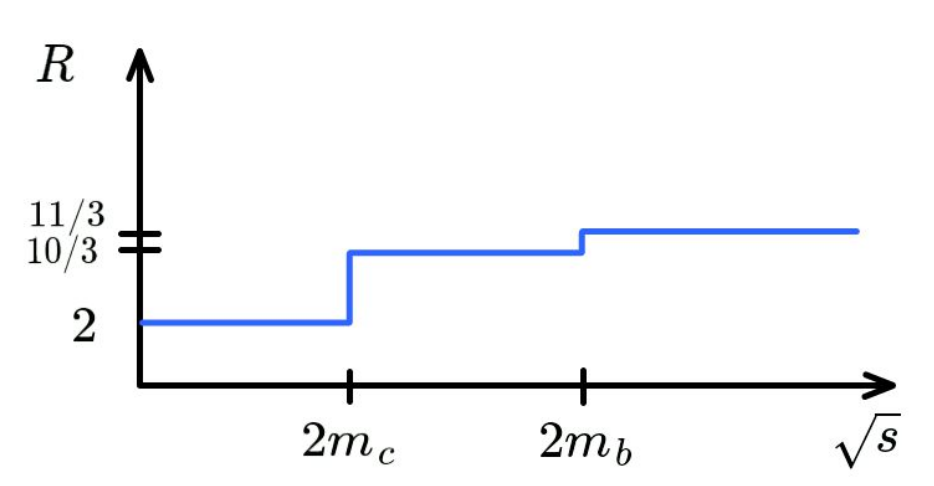
\includegraphics[scale=0.3]{images/Rratio.png}
\end{center}
\caption{Prediction for the $R$ ratio as a function of the centre of mass energy.}\label{fig:Rratio}
\end{figure}
%%\image{RratioExp.png}
\begin{figure}
\begin{center}
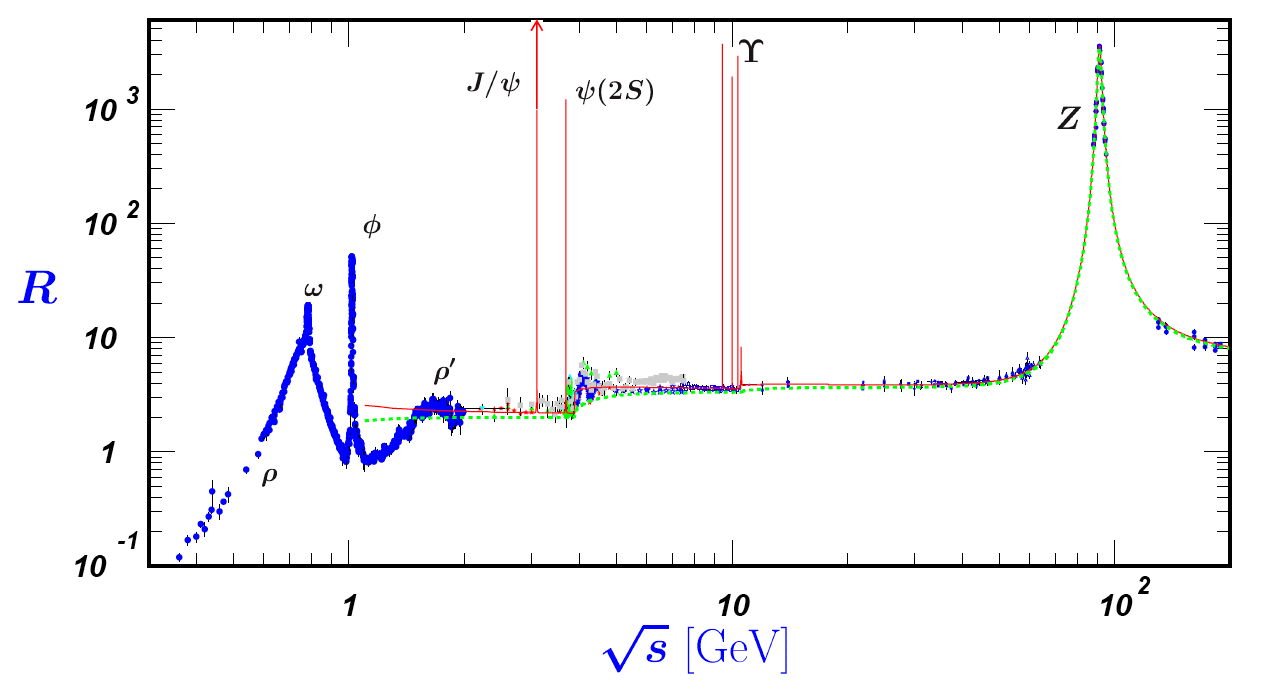
\includegraphics[scale=0.3]{images/RratioExp.png}
\end{center}
\caption{Experimental result for the $R$ ratio as a function of the centre of mass energy. The ratio is between the measured experimental cross section and the \emph{theoretical} cross section for $e^+e^-\rightarrow\mu^+\mu^-$, which does not contain the resonances. Plot from \cite{pdg}.}\label{fig:RratioExp}
\end{figure}


The differential cross section for the annihilation of an electron-positron pair into an muon-antimuon pair is given by
\[\frac{d\sigma(e^+e^-\rightarrow \mu^+\mu^-)}{d\Omega}=\frac{\alpha^2}{4s}\left(1+\cos^2\theta\right)\;,\] 
where we neglected the mass of the electron and muon and the contribution from the $Z$ boson. With these masses neglected the only quantity with units of energy is $s$. The factor $1/s$ in the cross section has the right power of energies to give the cross section its units of an area. The angle dependence comes from the fact that the muon pair comes from the decay of a virtual photon. We can integrate over the solid angle $d\Omega$ to obtain the total cross section:
\[\sigma(e^+e^-\rightarrow \mu^+\mu^-)=\frac{4\pi\alpha^2}{3s}\;.\]
\begin{figure}
\begin{center}
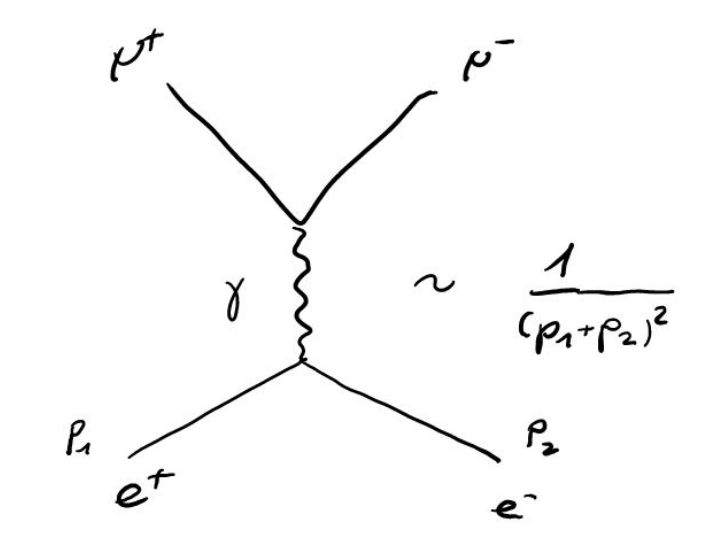
\includegraphics[scale=0.3]{images/eeYmumu.png}
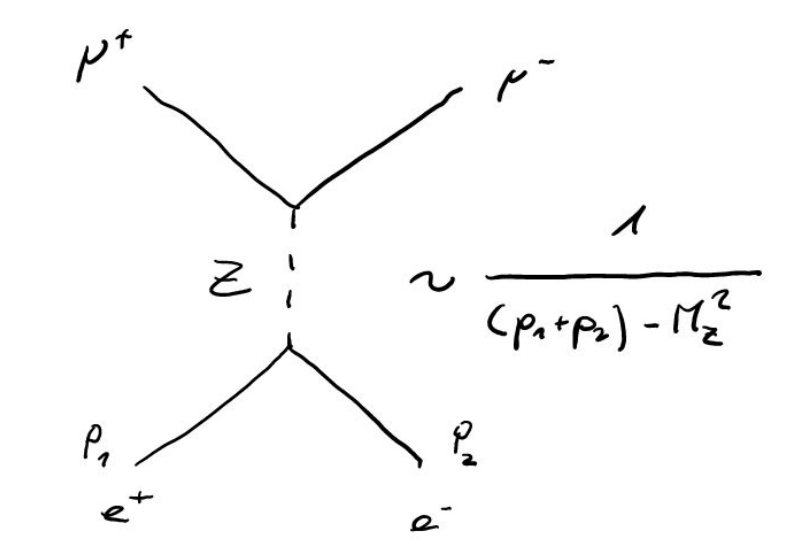
\includegraphics[scale=0.3]{images/eeZmumu.png}
\end{center}
\caption{Feynman diagrams for the annihilation of an $e^+e^-$ pair into a $\mu^+\mu^-$ pair. The left diagram shows the photon exchange, the right diagram the exchange of a $Z$ boson. The amplitudes for the two diagrams receive different factors from the propagator.}\label{fig:eemumu}
\end{figure}
We have neglected the $Z$ boson contribution depicted in figure~\ref{fig:eemumu}. The amplitude for this contribution contains a factor
\[\frac{1}{(p_1+p_2)^2-M_Z^2}\]
from the $Z$ boson propagator. The momentum carried by the $Z$ boson is the sum of the initial state particle's momenta $(p_1+p_2)$ and its square is the centre of mass energy squared $s$. For energies much lower than the $Z$ boson mass ($\simeq 90\,{\rm GeV}$) this is negligible and the cross section is proportional to 
\[\sigma \sim |\mathcal{M}|^2 \sim \left(\frac{1}{s-M_Z^2}\right)^2  \sim \frac{1}{M_Z^4}\;.\]
This is much suppressed compared to the same diagram with the photon where we have
\[\sigma \sim |\mathcal{M}|^2 \sim \left(\frac{1}{s}\right)^2  \sim \frac{1}{s^2}\;,\]
which is much larger for $\sqrt{s}\ll M_Z$.
%%\lecture{23}
\subsection{Resonances}
Looking at the experimental result for the $R$ ratio in figure~\ref{fig:RratioExp} we see that in the vicinity of the quark thresholds we observe resonances. They occur when the centre of mass energy $\sqrt{s}$ matches the mass of a $q\bar q$ bound state. At these energies a bound state is created and its decay into hadrons is measured.

The resonances have to have the same quantum numbers as the virtual photon, so the only mesons can be produced are electrically neutral vector mesons.   
%%\keypoint{ We see hadronic resonances in the hadron production, they correspond to the meson states with quantum numbers compatible with the photon ($J^P=1^-$), namely the vector mesons.}

The first two such mesons are the $\rho^0$ and the $\omega$ mesons. Their wave functions and main decay channel are
\begin{eqnarray*}
\rho^0:& \frac{1}{\sqrt{2}}\left(|u\bar u \rangle -|d\bar d \rangle \right)&
\qquad\rho^0\rightarrow \pi^+\pi^- \quad\quad(\sim 100\%)\\ 
\omega :& \frac{1}{\sqrt{2}}\left(|u\bar u \rangle +|d\bar d \rangle \right)&\qquad \omega \rightarrow \pi^+\pi^-\pi^0\quad(89\%)\;. 
\end{eqnarray*} 
The fact that the $\rho$ meson can decay into two pions and the $omega$ meson decays mainly into three pions is a consequence of isospin conservation of the strong force.

The next resonance is the $\phi$ vector meson:
\begin{eqnarray*}
\phi:& |s\bar s \rangle &
\qquad\phi\rightarrow K^+ K^- \quad\quad(\sim 49\%)\\ 
&&
\qquad\phi\rightarrow K^0 \bar K^0 \quad\quad(\sim 34\%)\\ 
\end{eqnarray*} 
At higher energies we have the resonances for the charmonium and bottomium bound states. Finally at energies around $90\,{\rm GeV}$ we have the $Z$-boson resonance. In this case the energy is very high and of the two diagrams in figure~\ref{fig:eemumu} the one with the $Z$ boson dominates.
%%\keypoint{At a centre of mass energy of $\sqrt{s}\simeq$ 91 GeV in $e^+e^-$ collisions we can produce a $Z$ boson.}
The non-relativistic cross section for a resonance of mass $E_0$ and width $\Gamma_{tot}$ is given by
\[\sigma_{i\rightarrow f}(E)=\frac{\pi\lambdabar (2J+1)}{(2s_a+1)(2s_b+1)}\frac{\Gamma_i \Gamma_f}{(E-E_0)^2+\Gamma_{tot}^2/4}\;,\] 
where $\lambdabar$ is the de Broglie wavelength of the incoming particles  $J$ is the spin of the resonance, $s_a$ and $s_b$ are the spins of the initial state particles. $\Gamma_{R\rightarrow i}$ and $\Gamma_{R\rightarrow f}$ are the partial width for the decay of the resonance $R\rightarrow i$ and $R\rightarrow f$:
%%\image{resonanceFormula.png}
\[\Gamma_{tot} = \sum\limits_{ {\rm decay\,channels}\,c} \Gamma_{R\rightarrow c}\]
The partial width are related to the matrix element or the decay process through
\[\Gamma_{R\rightarrow c}=\frac{(2\pi)^4}{2M}\int \left| \mathcal{M}(R\rightarrow c) \right|^2 \;d \phi\;,\]
where the integral is over the phase space of the decay particles. 

For an $e^+e^-$ collision where the energy is high enough to ignore the electron mass we have $J=1$, $s_a=s_b=1/2$, $\lambdabar=2/\sqrt{s}$. We also need to modify the formula for the cross section of the resonance to the relativistic case. We get for a resonance of mass $M_R$:
\[\sigma_{e^+e^-\rightarrow f}(s)=12\pi M_R^2\frac{\Gamma_{R\rightarrow i}\Gamma_{R\rightarrow f}}{(s-M_R^2)^2+M_R^2\Gamma^2_{tot}}\;.\] 
The cross section has a peak at $s=M_R^2$. The height of the peak is proportional to 
\[\sigma(s=M_R^2)\sim \frac{1}{\Gamma_{tot}^2}\;.\]
Since the lifetime is inverse proportional to the width this means that long lived particles have a small width and an high resonance peak while short-lived particles have a broad resonance with a lower peak. It is worth noting that the width of the peak is the total width regardless of the channel where the decay is measured. 
%%\keypoint{The height of the peak of resonances is related to the width of the resonance and the width of the resonance to decay into the initial and final states. The width of the resonance is the total width, in all channels, but the height can be different.}
\clearpage
%
%%\lecture{24}
%%\section{Weak interaction}
%
\section{Weak interaction}
Weak interactions are mediated by the $W^\pm$ and $Z^0$ bosons. It is the only interaction that can alter the flavour of quarks or exchange charged leptons and neutrinos. It is responsible the nuclear $\beta$ decays and the decay of heavy quarks and leptons. The interaction is much much weaker than the strong or electro-magnetic forces at low energies. The reason is that unlike the latter the weak interaction is carried by massive particles.
%%\keypoint{The weak interaction is mediated through the $W^{\pm}$ and $Z^0$ bosons, it is responsible to the nuclear beta decays and the decay of heavy quarks.}
\begin{center}
\begin{tabular}{c|c|c}
interaction & carrier & mass \\
\hline
\hline
strong  & gluon & 0 \\
\hline
electro-magnetic  & photon & 0 \\
\hline
      & $W^+$ & $80.4$ GeV \\
weak  & $W^-$ & $80.4$ GeV \\
      & $Z^0$ & $91.2$ GeV 
\end{tabular}   
\end{center}
\subsection{Leptons}
\subsubsection{Charged leptons}
There are three known charged leptons: the electron $e^-$, the muon $\mu^-$ and the tau lepton $\tau^-$ and each has its positively charged anti-particle: $e^+$, $\mu^+$ and $\tau^+$. 
%%\keypoint{There are three types of charged leptons, the electron ($e^-$), muon ($\mu^-$) and tau ($\tau^-$).}
\begin{center}
\begin{tabular}{c|c|c}
particle &  symbol & mass \\
\hline
\hline
electron  & $e^-$ & $0.511\,{\rm MeV}$ \\
\hline
muon  & $\mu^-$ &  $105.65\,{\rm MeV}$ \\
\hline
 tau     & $\tau^-$ & $1776.8\,{\rm MeV}$
\end{tabular}   
\end{center}
The charged leptons have the same quantum numbers, the only difference is that the muons and tau leptons are heavier than the electrons. The muons and taus can decay through the weak interaction to a lighter charged lepton.
\begin{eqnarray*}
\mu^-&\rightarrow&e^-\,\bar \nu_e \, \nu_\mu\\
\tau^-&\rightarrow&e^-\,\bar \nu_e \, \nu_\tau\\
\tau^-&\rightarrow&\mu^-\,\bar \nu_\mu \, \nu_\tau\\
\tau^-&\rightarrow& \pi^-\, \nu_\tau\;.
\end{eqnarray*}
%%\keypoint{The muon is heavier that the electron and can decay into the an electron, a neutrino and an anti-neutrino.}
%%\keypoint{The tau lepton is the heaviest and can decay into the lighter charged leptons and a neutrino and an anti-neutrino.}
One might wonder whether the muon and tau leptons are excited states of the electron. The electro-magnetic decay $\mu\rightarrow e^- \gamma$ has been searched for but not found which means that the muon is not an excited state of the electron.
\subsubsection{Neutrinos}
Neutrinos are electrically neutral and can only interact through the weak interaction. This fact makes their study challenging. In most cases they are observed indirectly by using conservation laws. One example is the beta decay where the neutrino momentum is such that the total momentum is conserved.
%%\keypoint{Neutrinos are electrically neutral particles that only interact weakly. They are fermions and they have an anti-particle. }
%%\keypoint{There is one type of neutrino for each type of charged lepton.}

Neutrinos are nearly massless, we don't know their masses but because we observe oscillations we know they have a mass. The current upper bound on the neutrino mass is about $2\;{\rm eV}$. For all collider and decay applications they can be treated as massless. 

The beta decay of a neutron is a source of neutrino, the reaction is
\[n\;\rightarrow\; p + e^-+\bar\nu_e\;.\]
This reaction occurs in very large number in a nuclear reactor, which makes them a good source of neutrinos. In this reaction we have an electron anti-neutrino and not just "a neutrino", in the follow we will see why these two distinctions are necessary. 

Using anti-neutrino from a nuclear reactor we can look for two reactions 
\begin{eqnarray*}
\bar\nu_e +p &\rightarrow& n+e^+\\
\bar\nu_e +n &\rightarrow& p+e^-\;.
\end{eqnarray*}
The first one is called inverse beta decay and has been observed. The other reaction has not been observed. If the neutrino was its own antiparticle one would expect to see this process and we can therefore conclude that the neutrino and the antineutrino are not the same particles. 
 
It has also been observed that neutrinos involved in reactions with an electron and not the same as the ones involved in reactions with a muon or a tau. We have therefore three different types of neutrino which we group with their associated charged lepton in three groups called generations:
\[
\left(\begin{array}{c}e^-\\ \nu_e \end{array}\right)\;,\qquad
\left(\begin{array}{c}\mu^-\\ \nu_\mu \end{array}\right)\;,\qquad
\left(\begin{array}{c}\tau^-\\ \nu_\tau \end{array}\right)\;.\qquad
\]  
%%\keypoint{ We can organise the leptons in "generations", one for the electron and electron neutrino, one for the muon and the muon neutrino and one for the tau and tau neutrino. }
The lepton and the neutrino from the same generation interact through the weak interaction and there is no interactions between leptons and neutrinos of different generations. 

In all reactions we have observed the creation annihilation of a lepton is always associated with the creation or annihilation of a neutrino of the same generation. We can formalise this fact by introducing a conserved quantum number, the lepton number:
\[L_l=N(l)-N(\bar l)+N(\nu_l)-N(\bar \nu_l)\;,\qquad l=e,\mu,\tau\;.\]
%%\keypoint{ We can associate an additive quantum number for each of these families with $N_l=+1$ for the charged lepton $l$ and its neutrino $\nu_l$ and $N_l=-1$ for the charged anti-lepton $l^+$ and the anti-neutrino $\bar{\nu}_l$. This quantum number is conserved in all interaction vertices, but over very long distances neutrino can oscillate from one flavour to the other, so that this violate individual lepton numbers.}
There is one lepton number per generation and they are all individually conserved in weak interaction vertices. The $\nu_e$, $\nu_\mu$, $\nu_\tau$ neutrinos are the eigenstates of the weak interaction, but they are not the mass eigenstates, so while propagating the flavour or a neutrino can change, leading the the observed phenomenon of \emph{neutrino oscillation}. We can define the total lepton number
\[L=L_e+L_\mu+L_\tau\]
which is also conserved in a neutrino oscillation. The mechanism behind the neutrino masses is not known and is the subject of current research.
%%\keypoint{The sum $L=L_e+L_\mu+L_\tau$ is conserved.}

The following processes are allowed by lepton number conservation:
\begin{eqnarray*}
p+\mu^-  &\rightarrow & \nu_\mu+n \\
e^++e^-  &\rightarrow & \nu_\mu+\bar \nu_\mu \;,  
\end{eqnarray*}
while the following processes are not allowed:
\begin{eqnarray*}
p+\mu^-  &\rightarrow & \pi^0 + n \\
e^++e^-  &\rightarrow & \nu_\mu+\bar \nu_e \;.
\end{eqnarray*}
%
%
\subsubsection{Charged currents}
%
%
%%\keypoint{The weak interactions can be divided into two types: the charged currents which involve the exchange of a $W^+$ or a $W^-$ boson, or the neutral currents that involve the exchange of a $Z^0$ boson.}
The $W^+$ or $W^-$ bosons can couple a charged lepton with its neutrino, or couple two quarks of different flavours.  
\begin{center}
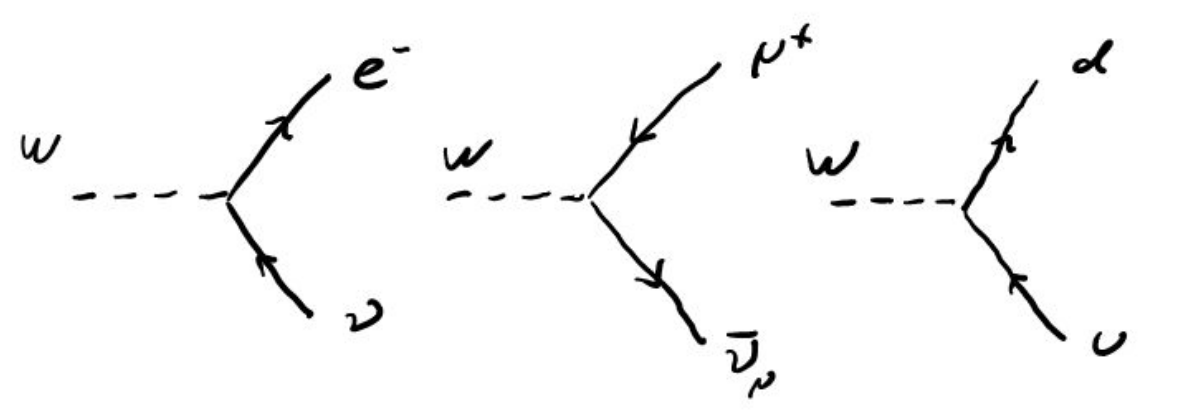
\includegraphics[scale=0.4]{images/Wvertices.png}
\end{center}    
The charge of on the fermion line changes by one unit so that together with the $W$ boson the total charge is conserved. Because the $W$ bosons carry one unit of electric charge an interaction mediated through a $W$ boson is called \emph{charged current}. Since the $W$ bosons couple to either leptons or quarks we have three combinations: 
\begin{description}
\item[leptonic processes] in which both ends of the $W$ boson propagator attach to a lepton line,
\item[semi-leptonic processes] in which one end of the $W$ boson propagator attach to a lepton line and the other to a quark line,
\item[non-leptonic processes] in which both ends of the $W$ boson propagator attach to a quark line.
\end{description} 
Examples of leptonic processes are the annihilation of a lepton with its antineutrino into a lepton and anti-neutrino of a different generation or the leptonic decay of the $\tau$-lepton.  
\begin{center}
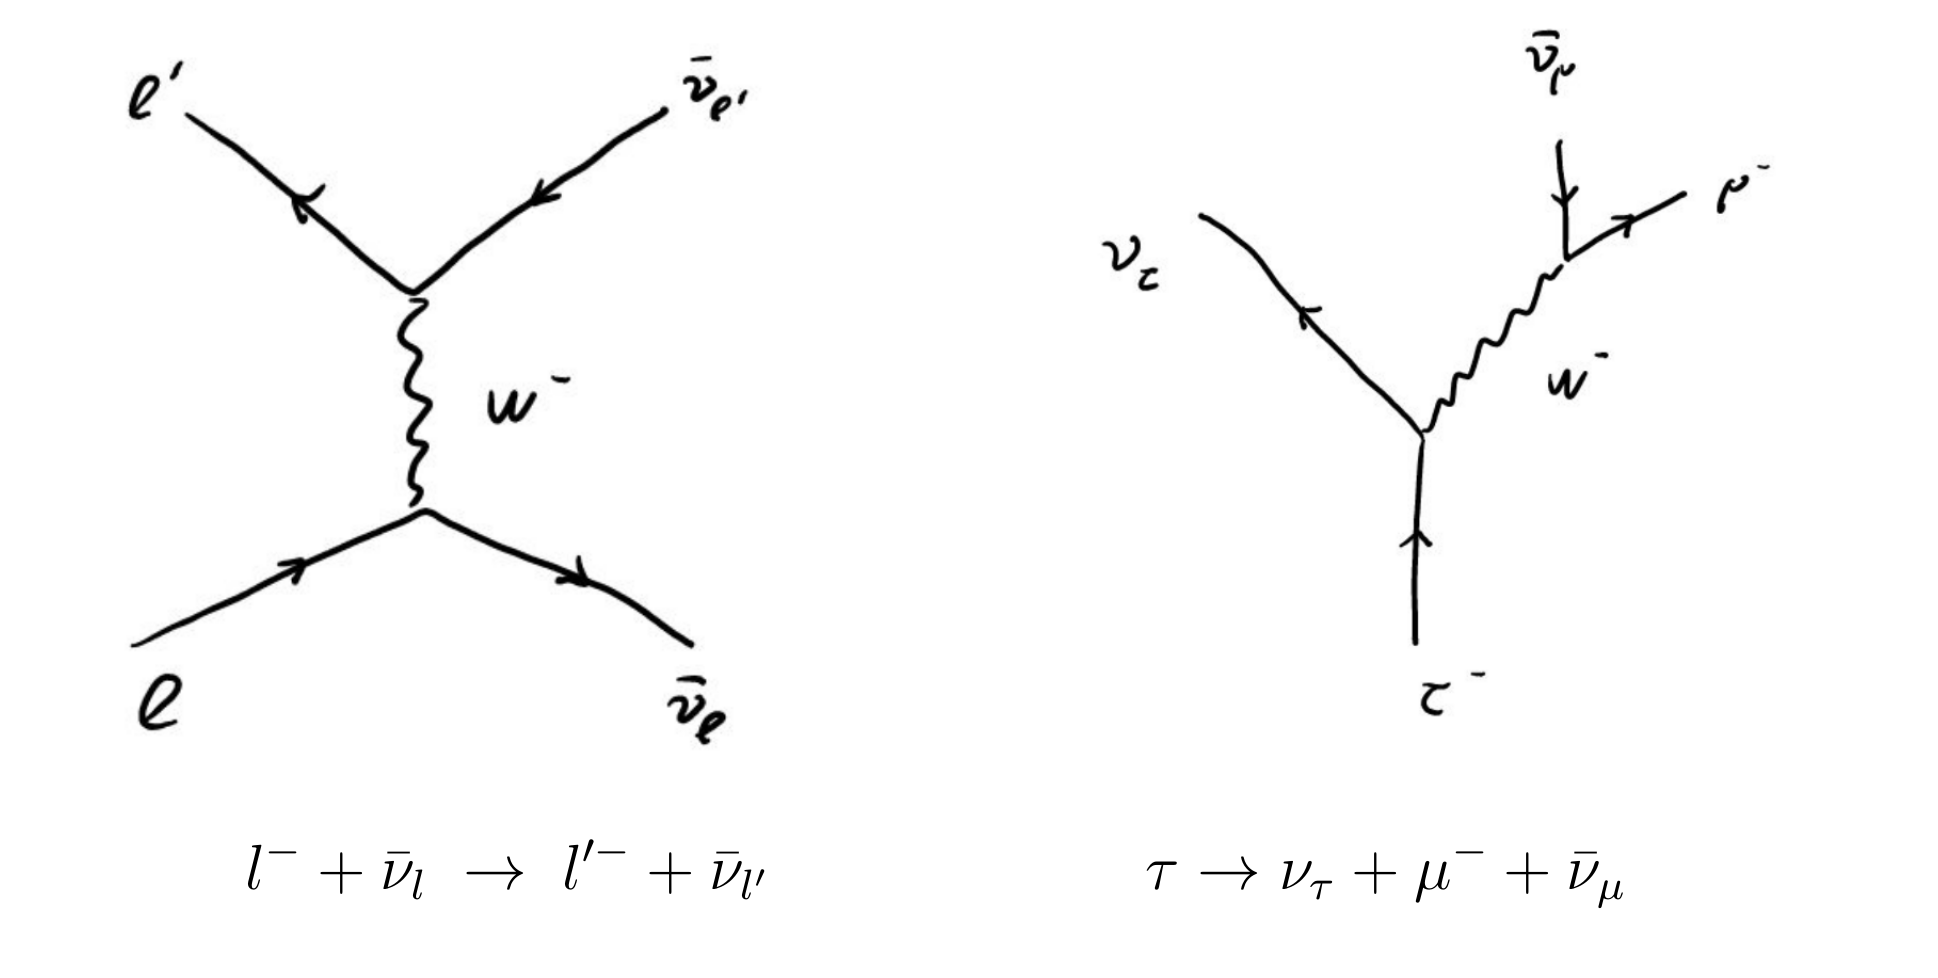
\includegraphics[scale=0.2]{images/WeakLeptonic.png}
\end{center}
\clearpage
Examples of semi-leptonic processes are the decay of the charged pions or the beta decay. 
\begin{center}
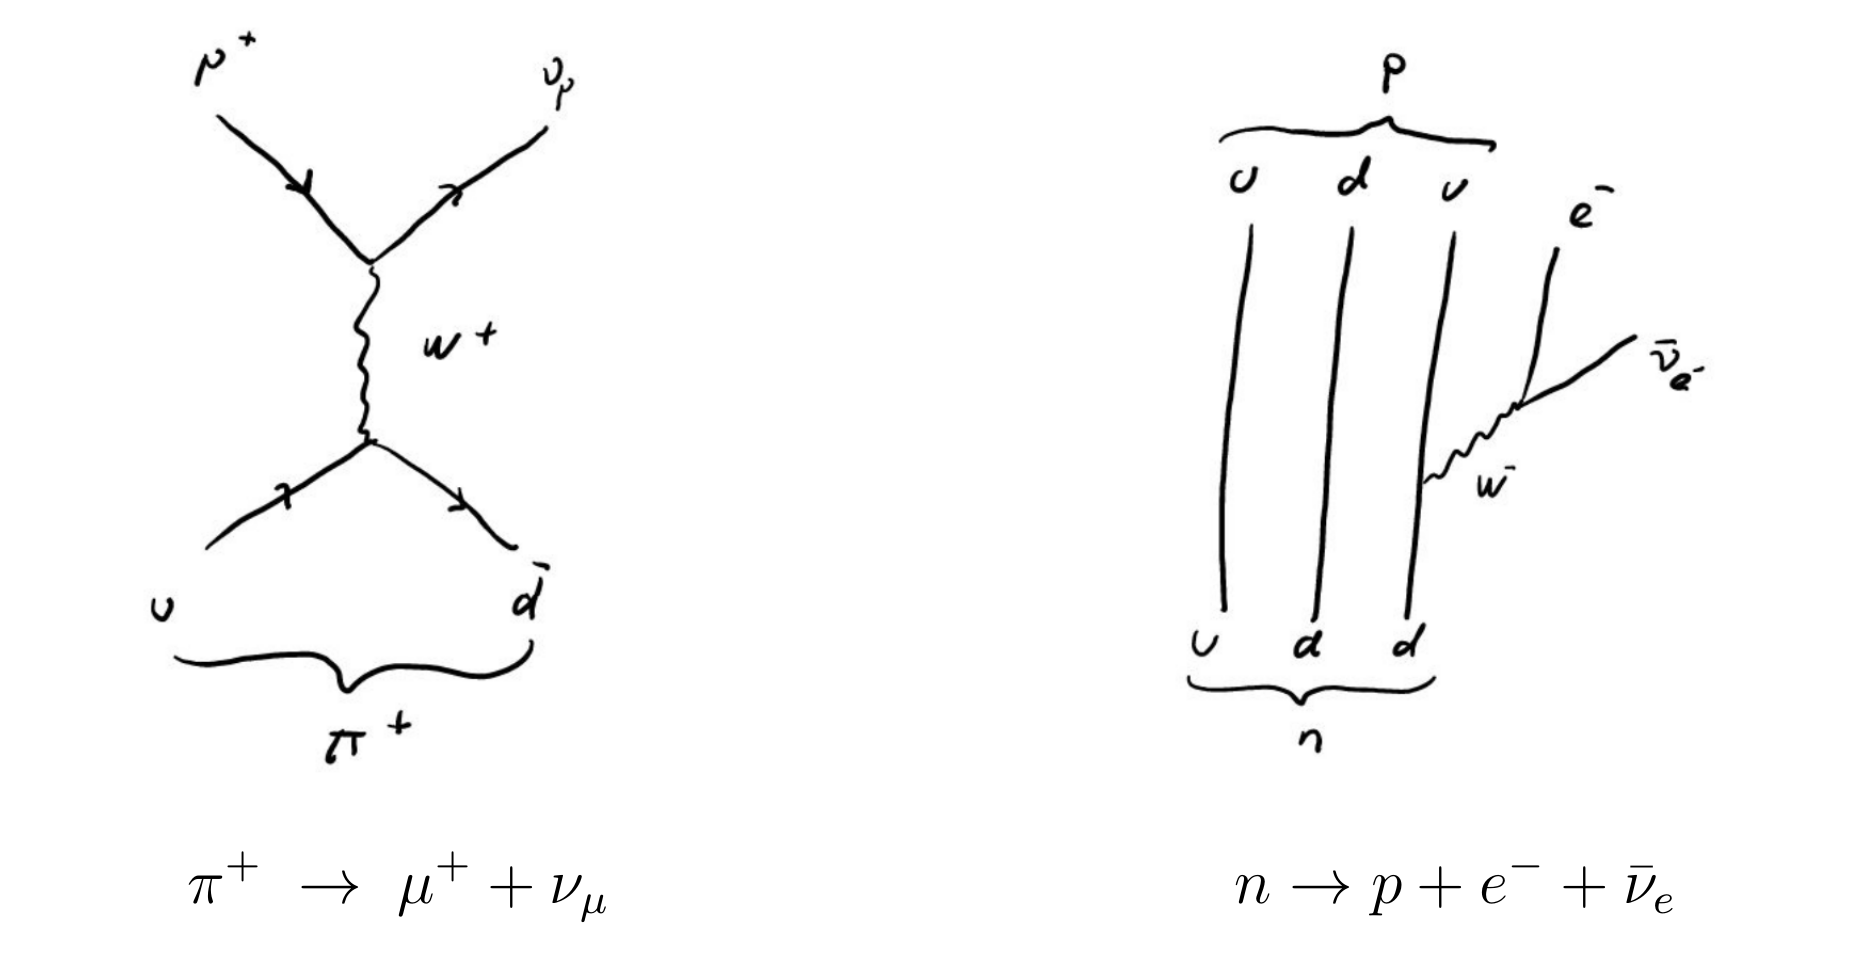
\includegraphics[scale=0.2]{images/WeakSemileptonic.png}
\end{center}
Examples of non-leptonic processes are weak decays of mesons or baryons containing heavy quarks. 
%%\image{Nonleptonic2.png}
\begin{center}
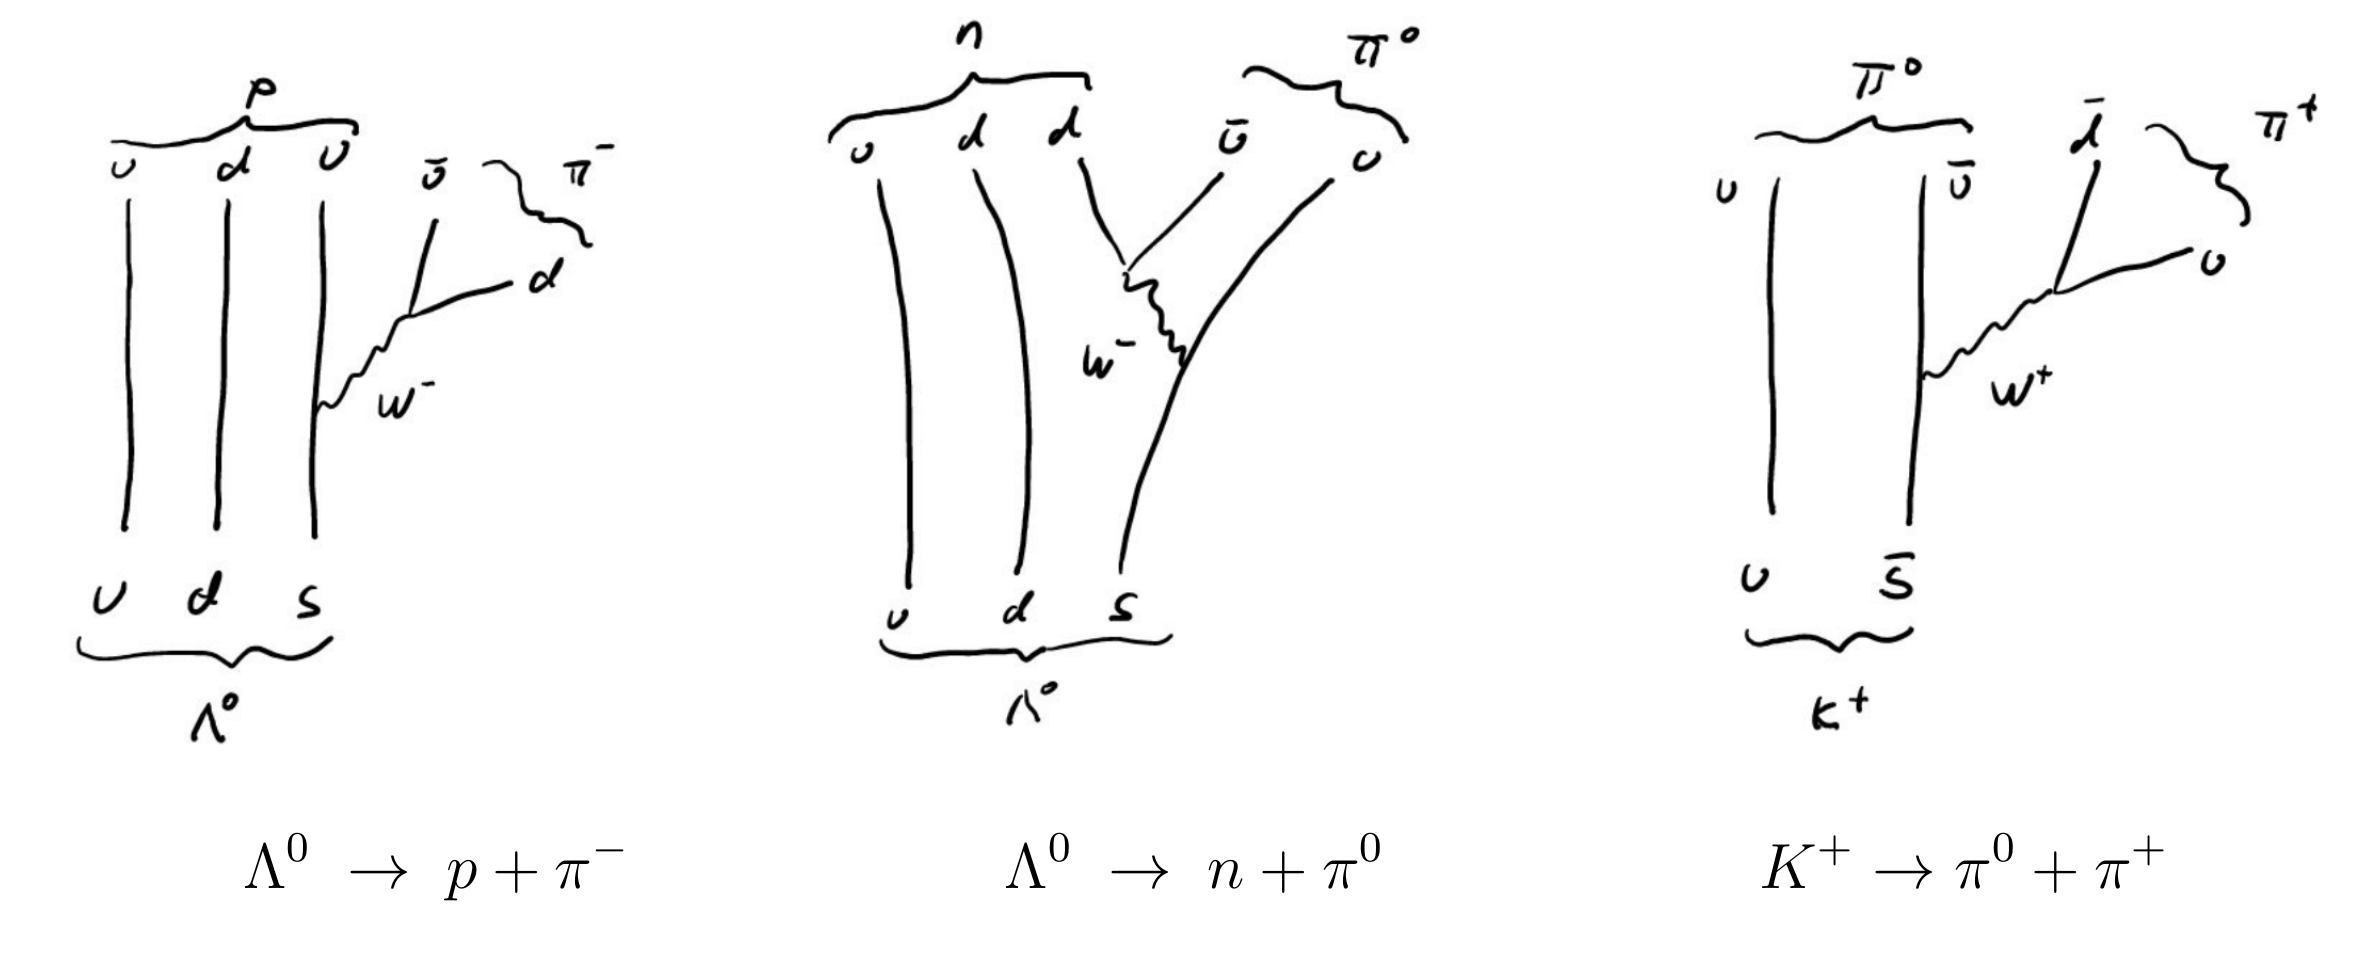
\includegraphics[scale=0.2]{images/WeakHadronic.png}
\end{center}
\subsubsection{Neutral currents}
The weak interaction can also be carried by the $Z^0$ boson. Unlike the $W$ boson there is no change of flavour when the $Z$ boson interacts with a lepton or a quark line. The $Z$ boson interacts with all charged particles and with the neutrinos. Because its mass is high, $M_Z=91.2 \;{\rm GeV}$, its effect is difficult to see because all processes that are allowed through a $Z$ boson exchange can happen through the exchange of a photon, with the exception of the interaction with neutrinos. 
%%\keypoint{A $W$ boson can interact with a charged lepton-neutrino pair or with a quark pair. As the charged current name hints, the interaction involves a change of charge for the members of the pair.}
\begin{center}
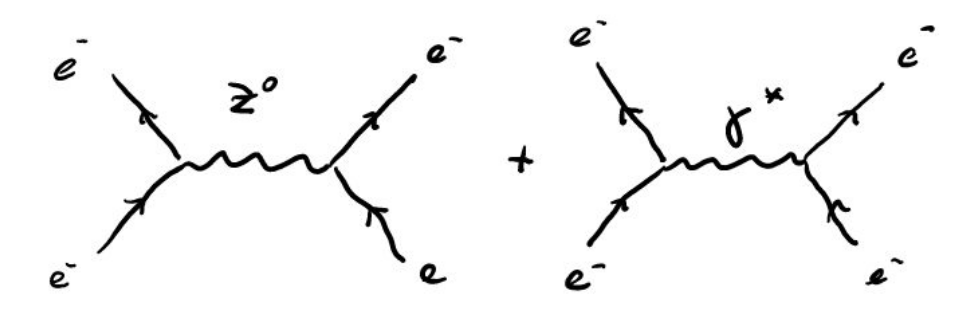
\includegraphics[scale=0.4]{images/eeeeZgamma.png}
\end{center}
At low energies the amplitude for the $Z$ boson exchange is suppressed by the $Z$ boson mass. At energies of the order of the $Z$ boson mass and higher the two processes are comparable in size. 
%%\keypoint{A $Z$ boson can interact with charged leptons, neutrinos, quarks and with a $W$ boson pair, but it cannot change the flavour of the particles it interacts with. A $Z$ boson cannot change the flavour of a quark or lepton it interacts with.}

In some cases involving neutrinos the $Z$ boson exchange is the only possibility, for example in the scattering of an electron and a muon neutrino, as shown in figure~\ref{fig:Zprocesses}.
\begin{figure}
\begin{center}
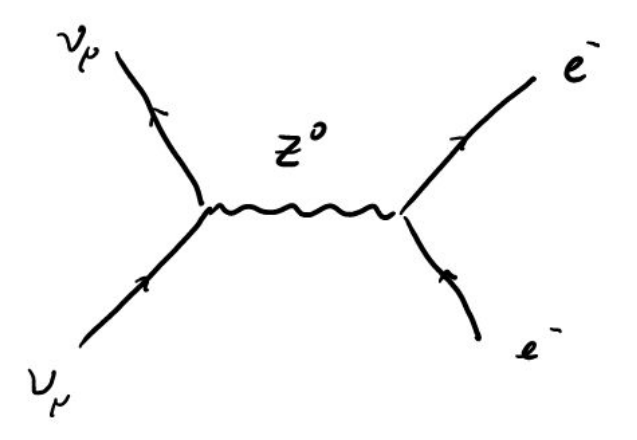
\includegraphics[scale=0.3]{images/enumuenumu.png}
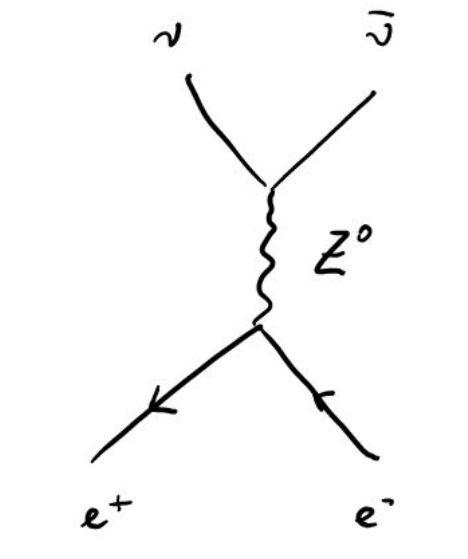
\includegraphics[scale=0.3]{images/eeZnunu.png}
\end{center}
\caption{Processes where the interaction of the $Z$ boson is important. Left: muon neutrino scattering off electrons, the $Z$ boson is the only particle that can mediate this interaction. Right: the annihilation of an electron-positron pair into a neutrino pair.}\label{fig:Zprocesses}
\end{figure}
Another place where the coupling of the $Z$ boson to the neutrinos is visible is in $e^+e^-$ collisions when a $Z$ boson is produced and it decays into neutrinos, as shown in figure~\ref{fig:Zprocesses}. The produced neutrinos will escape the detector undetected and no final state particle is seen. This process is usually called "$e^+e^-\rightarrow \mbox{invisible}$". Here again we must rely on indirect methods to prove the neutrino interaction: we can sum all partial widths for the visible decay of a $Z$ boson and notice that they do not sum up to the total width. By attributing the missing width to the decay into "invisible" neutrinos we can "count" the number of neutrinos and we indeed get three neutrino flavours.
%
%%\lecture{25}
\subsection{Coupling strength of the weak interaction}
%
%
The matrix element for the exchange of a $W$ boson contains a factor from the $W$ boson propagator:
%%\image{Wprop.png}
\begin{center}
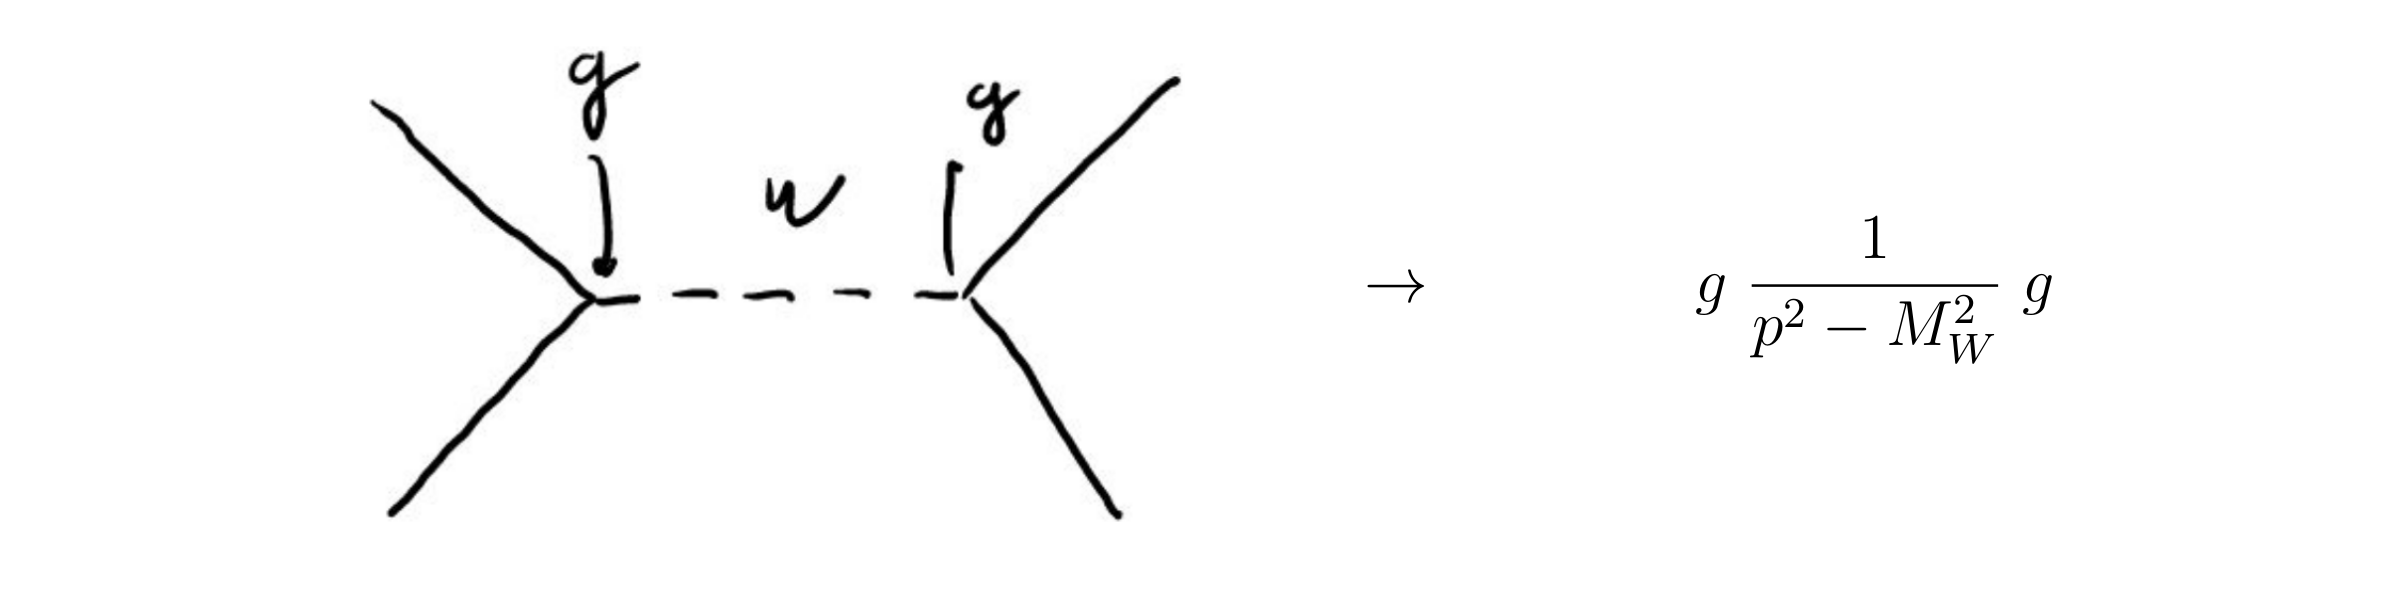
\includegraphics[scale=0.2]{images/WpropWithEq.png}
\end{center}
where we have neglected the $W$ boson width and where $p$ is the momentum carried by the $W$ boson. $g$ is the coupling strength, the equivalent for the weak interaction of the factor $\sqrt{\alpha}$ we have for the coupling of a photon to a fermion line. In the case of the photon we also had to multiply with the electric charge of the fermion the photon couples to, but we will see that in the case of the weak force all particles have the same weak charge. 

From the form of the propagator we see that in the limit where the $W$ boson carries a small momentum compared with the mass of the $W$ boson the latter dominates the denominator and the matrix element scales as
\[\mathcal{M}\sim \frac{g^2}{M_W^2}\;, \qquad\qquad\mbox{for}\qquad |p^2|\ll M_W^2\;.\]
pictorially we can understand this as "contracting" the $W$ boson propagator (as its momentum is negligible) to a point, as shown in figure~\ref{fig:fermi}.
%%\keypoint{At low energies the exchange of a $W$ boson can be seen as a $4$-fermion interaction with $G_F$ as its coupling strength.}
\begin{figure}
\begin{center}
\includegraphics[scale=0.2]{images/FermiTheory.png}
\end{center}
\caption{When the momentum of the $W$ boson is negligible the interaction looks like a four-fermion point interaction.}\label{fig:fermi}
\end{figure}  
The interaction then looks like a four-fermion interaction. Before the discovery of the $W$ boson the weak interactions were studied using such four fermion interactions. We can write the four fermion interaction coupling, called Fermi constant, in terms of the weak coupling and the $W$ boson mass:
\[\frac{G_F}{\sqrt{2}}=\frac{g^2}{M_W^2}\;,\]
where the factor of $\sqrt2$ is a convention and the units of the Fermi constant is ${\rm GeV}^{-2}$. We can measure $G_F$ in muon decays. The decay width of the muon is given to leading order as
\[\Gamma_\mu=\frac{1}{\tau_\mu}=\frac{G_F^2}{192\pi^3}m_\mu^5+\mathcal{O}(m_e/m_\mu)\;.\]
This formula neglects the mass of the electron compared to the mass of the muon. In this limit the mass of the muon is the only quantity with units of energy and we can deduce the dependence of the width on $m_\mu$: since the Fermi constant has units of inverse energy squared and the width has units of energy we need five powers of the muon mass to obtain the right units. The numerical value obtained is 
\[G_F=1.1663787\cdot 10^{-5}\,{\rm GeV^{-2}}\;.\]
We can use the decays of the $\tau^-$ lepton to compare the strength of the weak coupling to different particles:
\[\tau^-\;\rightarrow\;\nu_\tau \left\{ \begin{array}{c}
e^-+\bar \nu_e\\
\mu^-+\bar \nu_\mu\\
\pi^- (\bar u d)\\
\end{array} \right.
\;.\] 
These measurement show that the weak charge is the same for the leptons and the quarks.
%
%
\subsubsection{Quarks and the CKM matrix}
%
%
As for the leptons the quarks are organised into three generations:
\[
\left(\begin{array}{c}u\\ d \end{array}\right)\;,\qquad
\left(\begin{array}{c}c\\ s \end{array}\right)\;,\qquad
\left(\begin{array}{c}t\\ b \end{array}\right)\;.\qquad
\]  
We have seen that the weak interaction through the $W$ boson only coupled leptons within the generations. It is not the case for the quarks: the interaction within a generation is the most likely but interactions with other generations is possible, albeit less likely. This seems to be at odds with the previous result that the weak charge is the same for all particles. 
%%\keypoint{Each of the $u$,$c$,$t$ quarks can interact with any of the $d$,$s$,$b$ quarks through the exchange of a $W$ boson.}

The explanation is that the eigenstate of the weak interaction (which have the same weak charge as the leptons) are not the same as the eigenstates of the electro-magnetic interaction (that is the $u$, $d$, ... quarks). This solution was first proposed for the $u$, $d$, $s$ and $c$ quarks by Cabibbo. We can write the weak eigenstates $|d'\rangle$ and $|s'\rangle$ in terms of the $|d\rangle$ ,$|s\rangle$ eigenstates of the electro-magnetic interaction:
\[
\begin{array}{ccc}
|d'\rangle &=& \cos\Theta_c |d\rangle+\sin\Theta_c |s\rangle\\ 
|s'\rangle &=& -\sin\Theta_c |d\rangle+\cos\Theta_c |s\rangle 
\end{array}\;,\qquad\qquad
\begin{array}{ccc}
|d\rangle &=& \cos\Theta_c |d'\rangle-\sin\Theta_c |s'\rangle\\ 
|s\rangle &=& \sin\Theta_c |d'\rangle+\cos\Theta_c |s'\rangle 
\end{array}\;.
\]  
The coefficients are written in terms of an angle $\theta_c$, the Cabibbo angle. Numerically we have
\[\sin \theta_c\simeq 0.22\;,\qquad \cos\theta_c\simeq0.98\;.\]
If we now say that the $u$ quark couples through the $W$ boson to the $|d'\rangle$ only and the $c$ couples to the $|s'\rangle$ only. 
\begin{figure}
\begin{center}
\includegraphics[scale=0.2]{images/cabibbo.png}
\end{center}
\caption{Different processes with different contribution from the Cabibbo angle.}\label{fig:cabibbo}
\end{figure}
We can see in figure~\ref{fig:cabibbo} examples of processes and the effect of the Cabibbo angle. Leptonic processes are not affected, semi-leptonic and non-leptonic processes acquire one or two factors of either $\sin\theta_c$ or $\cos\theta_c$. Processes with a power of $\sin\theta_c$ are called "Cabibbo suppressed".
%%\keypoint{By realising that the weak eigenstates do not have to be the same as the EM and strong eigenstates we can build linear combinations of the $d$,$s$ and $b$ quarks in a way such that the interaction of the $u$,$c$,$t$ quarks is only with one of the combinations.}

With the discovery of the third generation of quarks this model had to be extended. The Cabibbo $2\times 2$ matrix is replaced by a $3\times 3$ matrix, the Cabibbo-Kobayashi-Maskawa matrix (for short "CKM matrix"):
\[
\left(\begin{array}{c}
|d'\rangle \\ 
|s'\rangle \\ 
|b'\rangle 
\end{array}\right)
=\left(\begin{array}{ccc}
V_{ud}&V_{us}&V_{ub}\\
V_{cd}&V_{cs}&V_{cb}\\
V_{td}&V_{ts}&V_{tb}
\end{array}\right)
\left(\begin{array}{c}
|d\rangle\\ 
|s\rangle\\ 
|b\rangle
\end{array}\right)
\]
%%\keypoint{The matrix of the basis change from EM and strong eigenstates to the weak interaction eigenstates is the CKM matrix.}
The CKM matrix is unitary so we have 
\[
\left(\begin{array}{c}
|d\rangle \\ 
|s\rangle \\ 
|b\rangle 
\end{array}\right)
=\left(\begin{array}{ccc}
V_{ud}^*&V_{cd}^*&V_{td}^*\\
V_{us}^*&V_{cs}^*&V_{ts}^*\\
V_{ub}^*&V_{cb}^*&V_{tb}^*
\end{array}\right)
\left(\begin{array}{c}
|d'\rangle\\ 
|s'\rangle\\ 
|b'\rangle
\end{array}\right)
\]
As for the two-flavour case different processes get different contributions from the CKM matrix, as shown in figure~\ref{fig:CKMprocesses}
\begin{figure}
\begin{center}
\includegraphics[scale=0.2]{images/CKMVubVcb.png}
\end{center}
\caption{CKM matrix contribution to two different $b$ quark decay.}\label{fig:CKMprocesses}
\end{figure}
The top left part of the CKM matrix corresponds to the matrix we had for the two-flavour case. The relative size of the matrix elements of the CKM matrix are shown in figure~\ref{fig:CKMsize}. The diagonal elements corresponding to interactions between quarks of the same generation are the largest, matrix elements corresponding to interaction between neighbouring generations are smallest but the elements corresponding to a change from the lightest generation to the heaviest are smallest. 
%%\keypoint{The CKM matrix can explain different probability for weak processes involving different quark flavours.}
%%\image{CKMsize.png}
\begin{figure}
\begin{center}
\includegraphics[scale=0.4]{images/CKMsize.png}
\end{center}
\caption{Size of the CKM matrix elements.}\label{fig:CKMsize}
\end{figure}

\clearpage
%%\lecture{26}
%%\section{Parity violation}
\subsection{Parity violation}
Parity is the symmetry associated with space inversion. Under a parity transformation vector-like quantities get a minus sign, for example
\[\vec x,\vec p\quad \longrightarrow \quad -\vec x,-\vec p \;,\]
and axial-vector quantities (also called pseudo-vector) such as angular momenta are invariant
\[\vec L,\vec S,\vec J \quad\longrightarrow\quad \vec L,\vec S,\vec J\;,\]
scalar quantities such as the mass or the charge are invariant. Pseudo-scalar quantities acquire a minus sign under a parity transformation. On example of such a quantity is the helicity of a particle. The helicity is defined as
\[h=\frac{\vec s\cdot \vec p}{|\vec s||\vec p|}\;,\] 
where $\vec s$ is the spin of the particle and $\vec p$ its momentum. 

If we consider a a massless fermion and measure its helicity (which means we are measuring its spin along the direction of its momentum) we can get either $h=+1$ or $h=-1$. 
\begin{center}
\includegraphics[scale=0.2]{images/LRhanded.png}
\end{center}
A massless fermion with helicity $h=+1$ is called "right-handed"  and if $h=-1$ it is called "left-handed". A parity transformation changes a right-handed fermion into a left-handed one and vice-versa. 
%%\keypoint{The helicity of a particle is given by the projection of the spin measured along the momentum direction divided by the magnitude of the spin. Massless particles with spin aligned with the momentum are called right-handed and those with spin anti-aligned with their momentum are called left-handed. Left handed and right-handed states are related through parity.}

To see what happens to the anti-fermion let us consider the Feynman diagram of figure below. 
\begin{center}
\includegraphics[scale=0.2]{images/LRfermionAntifermion.png}
\end{center}

They are equivalent, the only difference is that we read it either with the time flowing from the left to the right or from the bottom to the top of the page. Since the amplitude for the two amplitude are equivalent we see that a left-handed fermion is equivalent to a right-handed anti-fermion. By comparing the same Feynman diagram read in different time directions one can see that a right-handed fermion is equivalent to a left-handed anti-fermion.

For massless fermions the helicity is Lorentz invariant and is an appropriate quantum number: a massless fermion can be either right-handed or left-handed.

We can separate an interaction in two different part, depending on how the interaction treats left- and right- handed particle, it can be a: 
\begin{description}
\item[vector interaction: ] has coupling between particles of the same handedness, that is between 

\[\begin{array}{ccc}
f_L & \mbox{and} & f_L\\
f_R & \mbox{and}& f_R\\
f_L & \mbox{and}& \bar f_R\\
%\bar f_R & \mbox{and}& f_L\\
\bar f_R & \mbox{and}& \bar f_R\\
f_R & \mbox{and}& \bar f_L\\
%\bar f_L & \mbox{and}& f_R\\
\bar f_L & \mbox{and}& \bar f_L\\
\end{array}\]

\item[axial-vector interaction: ] has coupling between particles of opposite handedness, that is between 

\[\begin{array}{ccc}
f_L & \mbox{and} & f_R\\
f_R & \mbox{and}& f_L\\
f_L & \mbox{and}& \bar f_L\\
%\bar f_R & \mbox{and}& f_R\\
\bar f_R & \mbox{and}& \bar f_L\\
f_R & \mbox{and}& \bar f_L\\
%\bar f_L & \mbox{and}& f_R\\
\bar f_L & \mbox{and}& \bar f_L\\
\end{array}\]
\end{description}
Each interaction can be split into a vector and axial-vector part and we can quantify their strength with a vector coupling $c_V$ and an axial-vector coupling $c_A$. 

An interaction conserves parity if it is either purely vector ($c_V=1$, $c_A=0$) or purely axial-vector ($c_V=0$, $c_A=1$). If both $c_V$ and $c_A$ are non-vanishing, then parity is violated.  

Parity is maximally violated in the two following cases:
\begin{description}
\item[$c_A=c_V$] this case is called a "V+A" coupling, in this case we have an interaction between right-handed fermions and left-handed antifermions and no interaction between left-handed fermions and right-handed antifermions.  
\item[$c_A=-c_V$] this case is called a "V-A" coupling, in this case we have an interaction between left-handed fermions and right-handed antifermions and no interaction between right-handed fermions and left-handed antifermions.  
\end{description}
Here we have described the interaction in terms of a fermion and an anti-fermion but the equivalent interaction between two fermions or two antifermions has the same property. 
\begin{center}
\begin{tabular}{|c|c|c|c|c|}
\hline 
interaction & $f_L\; \bar f_L$ & $f_L\; \bar f_R$ &$f_R\; \bar f_L$ & $f_R\; \bar f_R$ \\ \hline
$V$  & no  & yes & yes & no \\
$A$  & yes  & no & no & yes \\
$V+A$  & no  & no & yes & no \\
$V-A$  & no  & yes & no & no \\\hline
\end{tabular}
\end{center}

A "V-A" coupling is also called "left-handed" coupling and a "V+A" coupling is called "right-handed" coupling.

It turns out that the coupling through a $W^\mp$ boson is a "V-A" coupling, which means parity is not only violated but maximally violated. This means that the $W$ bosons only couple to left-handed neutrinos and right-handed anti-neutrinos. Experimentally all neutrinos we have observed so far are left-handed. Right-handed neutrinos (and left-handed antineutrinos) might exist but they do not interact through the weak force.
%%\keypoint{The weak interaction only couples left-handed particles and right-handed anti-particles. The explicitly violates parity.}
%%\keypoint{Because the weak interaction only couples to LH neutrinos and RH anti-neutrinos, right-handed neutrinos, if they exist, do not interact with conventional matter.}

So far we have only treated massless fermions. For a massive particle the situation is more complicated: the weak force still only couple to left-handed fermions (and right-handed anti-fermions), but the left-handed state is a mixture or positive and negative helicity. The reason is that the interaction is Lorentz invariant, but the helicity is not. We can understand that helicity is frame dependent by imagining a massive particle travelling in one particular direction, because this particle is massive it is not travelling at the speed of light, which means we can perform a frame change that "overtakes" the particle, such that in this frame the particle would move in the opposite direction. Since this frame change does not change the spin direction the helicity is reversed. We can write the LH state (the one interacting with the $W$ boson) in terms of helicity states:
\begin{equation}
f_L=c\left|h=-1 \right> + c'\left|h=+1 \right>\;,
\qquad
f_R=c\left|h=+1 \right> + c'\left|h=-1 \right>\;.
\end{equation}\label{eq:fLRhel}
where the coefficients are 
\[
c=\frac{1}{2}\left(1+\frac{|\vec p|}{E+m}\right)\;,
\qquad
c'=\frac{1}{2}\left(1-\frac{|\vec p|}{E+m}\right)\;.
\]
We can see that in the massless limit we recover the case where the helicity states match exactly the LH and RH states.
%%\keypoint{For massive particles the helicity is a frame-dependent quantity. One can define right handed and left-handed states for them as a linear combination of helicity states and the weak interaction only couples to the left-handed fermion states and to the right-handed anti-fermion states.}
%
%
\subsection{Parity violation in decays}
%
%
\subsubsection{Pion decay}
The $\pi^\pm$ mesons have spin 0, they cannot decay electro-magnetically or through the strong force. We consider the decay of the negative pion $\pi^-$ to a charged lepton-antineutrino pair.
\begin{center}
\includegraphics[scale=0.4]{images/PionDecay.png}
\end{center}
Because the spin of the pion is 0, the lepton and neutrino have to have spins in opposite direction. Because the decay is mediated by the weak force the anti-neutrino has to be right-handed, that is its spin is aligned with its momentum. Because the spins have to be opposite the charged lepton $l$ also has to have positive helicity. This positive helicity state is the smaller part of the LH state that participates to the interaction. This part is smallest the lighter the lepton is. In the limit where the lepton is massless there would be no overlap between the LH state that takes part in the interaction and the positive helicity state in the final state so there would be no decay! More quantitatively the factors $c'$ in equation~\ref{eq:fLRhel} are for the electron and the muons:
\[
e^-:\quad c'\simeq 0.00377 \;,
\qquad
\mu^-:\quad c'\simeq 0.44 \;.
\]
This means that the decay of the pion into an electron and an electron anti-neutrino is very much suppressed compared to the decay into a muon and muon anti-neutrino. 
%%\keypoint{Because the fraction of the LH states that has positive helicity is proportional to the mass of the particle weak processes for which angular momentum conservation forces a high energy fermion to have positive helicity are suppressed.}
The branching fraction of the pion decay into the electron and electron antineutrino is 
\[B(\pi^-\rightarrow e^-\bar \nu_e)\simeq0.0123\%\;,B(\pi^-\rightarrow \mu^-\bar \nu_\mu)\simeq 100\%\;.\]   
\subsubsection{Muon decay}
If we now look at the decay of a muon and consider the configurations in which the electron flies either in the direction of the of the muon spin or opposite to it we will see another effect of parity violation in weak decays. We look at the configuration in which the electron has the maximum energy, that is when both the muon neutrino and the electron antineutrino have momenta opposed to the electron momentum, as depicted below.
%%\image{MuonDecay.png}
\begin{center}
\includegraphics[scale=0.4]{images/MuonDecay.png}
\end{center}
Because the neutrinos are produce through the weak interaction the muon neutrino has to be left-handed and the electron anti-neutrino has to be right-handed. If both fly in the same direction their spins cancel and the electron has to have its spin in the same direction as the spin of the original muon. In the case where the electron goes in the direction of the muon spin (left in the picture above), this means the electron has positive helicity. In the other case (right in the picture above) the electron has negative helicity. In the first case the electron has the "wrong" helicity so that the amplitude for the decay is suppressed, while in the second case the electron has negative helicity, which has the most overlap with the LH state that participates in the interaction, so the decay is very likely. 

If one generates a polarised beam of muons (that is a beam of muons with a preferential direction of their spins), one can see that the electrons are more likely to be emitted against the direction of the muon spin.
%
%%\lecture{27}
%%\section{CP violation}
\subsection{CP violation}
%
%  
The charge conjugation operator $C$ changes a particle into its anti-particle, for the fermions it means
\[\begin{array}{ccccccc}
 f_R & \xrightarrow{C}&\bar f_R   &\qquad\qquad &    \bar f_R & \xrightarrow{C}& f_R \\
f_L & \xrightarrow{C}&\bar f_L    &&    \bar f_L & \xrightarrow{C}& f_L
\end{array}\]
Since the $W$ bosons couple to the left-handed fermions and the right-handed antifermions and not the the right-handed fermions and left-handed antifermions charge conjugation is also violated. What about the combination of $C$ and the parity operation $P$? 
%%\keypoint{ Because the weak interaction only couples LH fermions and RH anti-fermions the charge conjugation symmetry is also violated.}

The neutrinos (antineutrinos) of one handedness get transformed into antineutrinos (neutrinos) of the opposite handedness.  
\[\begin{array}{ccccc}
\nu_L & \xrightarrow{P}&\nu_R & \xrightarrow{C}&\bar\nu_R \\
\nu_R & \xrightarrow{P}&\nu_L & \xrightarrow{C}&\bar\nu_L 
\end{array}\]
The combination of the two transformation transforms particles into particles with the same coupling to the $W$ boson, so the combination $CP$ seems to be conserved, at least in the lepton sector. The situation gets more complicated for the quarks, as the electro-weak eigenstates are not the mass eigenstates.
%%\keypoint{The combination $CP$ of charge conjugation and parity is conserved in the lepton sector}
%
%
\subsubsection{CP-violation in neutral kaons}
%
%
The two neutral kaons $K^0$ and $\bar K_0$ can mix. They have different strangeness so we know the mixing is through the weak interaction. Two Feynman diagram for the mixing are shown below.
\begin{center}
\includegraphics[scale=0.3]{images/KaonMixing.png}
\end{center}
The $K^0$ and $\bar K_0$ can decay into a two- or a three-pion final state. The decay into two pions is more likely (therefore quicker) because the two-particle phase-space is larger than the three-particle phase-space.

The two- an three-pions final states are CP eigenstates. Applying $C$ to the $K^0$ we get a $\bar K^0$:
\begin{eqnarray*}
CP|\pi^0\pi^0\rangle &=& +1 |\pi^0\pi^0\rangle\\
CP|\pi^0\pi^0\pi^0\rangle &=& -1 |\pi^0\pi^0\pi^0\rangle
\end{eqnarray*}
but the $K^0$ and $\bar K^0$ are not:
\[C|K^0\rangle =  |\bar K^0\rangle\qquad\]
where we could have chosen a different phase. Applying parity we get:
\begin{eqnarray*}
CP|K^0\rangle &=& -1 |\bar K^0\rangle\\
CP|\bar K^0\rangle &=& -1 |K^0\rangle
\end{eqnarray*}
If $CP$ is to be conserved we need the particle that decays to be $CP$ eigenstates build from the $K_0$ and $\bar K^0$. This can be achieved through the combinations
\begin{eqnarray*}
|K^0_1\rangle &=& \frac{1}{\sqrt{2}}\left( |K^0\rangle  - |\bar K^0\rangle \right)\\
|K^0_2\rangle &=& \frac{1}{\sqrt{2}}\left( |K^0\rangle  + |\bar K^0\rangle \right)\\
\end{eqnarray*}
These combinations are $CP$ eigenstates:
\begin{eqnarray*}
CP|K^0_1\rangle &=& +1 |K^0_1\rangle  \\
CP|K^0_2\rangle &=& -1|K^0_2\rangle   \\
\end{eqnarray*}
If $CP$ is conserved we have the following decays:
\begin{eqnarray*}
|K^0_1\rangle &\rightarrow& |\pi^0\pi^0\rangle 
\qquad \qquad\mbox{short lived}
\\
|K^0_2\rangle &\rightarrow& |\pi^0\pi^0\pi^0\rangle  
\qquad \qquad\mbox{long lived}
\end{eqnarray*}
Kaons can be produced in a high energy collision of a proton with neutrons in a target. The kaons are created through a strong interaction as $K^0$, they then propagate as $CP$ eigenstates $K_1^0$ or $K_2^0$. What we expect is to have the $K_1$ decay quickly in two pions, while the $K_2$ propagate much further and decay into three pions. 
\begin{center}
\includegraphics[scale=0.4]{images/KSKL1.png}
\end{center}
Experiments showed that we indeed have a short lived neutral kaon and a long lived one called $K_S^0$ and $K_L^0$ with decays into two pions and three pions respectively, but a small fraction of $K_L$ are also observed to decay into a two-pion final state. This means that the $K_S^0$ and $K_L^0$ are not the $CP$ eigenstates $K_1^0$ and $K_2^0$. This means that $CP$ is not conserved! 
\begin{center}
%%\image{KSKL2.png}
\includegraphics[scale=0.4]{images/KSKL2.png}
\end{center}

$CP$ violation has been observed not only in the neutral kaons but also in $B^0-\bar B^0$ and $D^0-\bar D^0$ systems. From a theoretical point of view $CP$ violation is possible because of the possibility of having a non-trivial phase in the CKM matrix. This is only possible for three or more generations. 

While it might sound bad that $CP$ is violated, it is necessary to have some $CP$ violation in order to explain why we have a large surplus of matter compared to antimatter in the universe. In fact the $CP$ violation in the CKM matrix is not enough to explain this imbalance and it is the topic of current research to find more $CP$ violation. 
%%\keypoint{$CP$ is violated in the quark sector because of a small phase in the CKM matrix.}
 

\clearpage
\section{Key points}
\subsection{Deep inelastic scattering}
\begin{itemize}
\item In a deep inelastic experiment one collides an electron with a proton.
\item At low energies one sees an elastic scattering of the electron off the proton.
\item At moderate energies the electron can transfer enough energy to excite the nucleon to excited states (some of them are the $\Delta$ baryons).
\item At higher energies the electron recoils against point-like objects inside the proton.
\item These constituents are spin $1/2$ particles.
  \item The parton model stipulates that the proton is made up from constituent particles called partons (we know now that they are quarks and gluons) 
  \item The constituents have a momentum fraction distribution described by parton distribution functions.
    \item There are two types of quarks in a nucleon: the valence quark that give the quantum numbers of the nucleon and the sea quarks that come in pairs and don't give a net contribution to the quantum numbers of the nucleon.
  \item We can get information about the parton distribution functions using DIS with different targets and using electrons or neutrinos in the collision.
  \item The total momentum fraction carried by the quarks in a nucleon is about 1/2. Which means that the rest should be carried by particles with no electric of weak charges.
  \item We need to introduce a new quantum number to accommodate for the $\Delta^{++}$ resonance.
  \item Quarks and gluons carry colour charges. Quarks can have one of three colours, antiquarks carry anti-colour charges and gluons carry a colour-anticolour charge.
  \item Gluons are the carriers of the strong interaction. Since gluons also carry colour charges, they can interact between themselves, which photons cannot. One consequence is that the strong coupling is increasing as the energy lowers (which means that the distance increases)
  \item Only colour neutral objects can exist at a scale of $\simeq \, 1\,\rm{fm}$.
    \item The parton distribution functions have a mild energy dependence, this is due to the fact that at a larger energy we can resolve more of the cloud of sea quarks and gluons present in the nucleon.
\end{itemize}
    \subsubsection{Check questions}
  \begin{itemize}
\item Can you explain the different type of behaviour of the scattering at different energies in  terms of the wavelength of the exchanged photon?
\item How do we know that in DIS the electrons recoil against point-like particles?
\item How do we know that the constituents struck in DIS are spin $1/2$ particles?
\item How would the parton distribution functions look like if the three valence quarks were sharing the proton's momentum equally?
\item How do we know that the total momentum fraction carried by the quarks in a nucleon is about 1/2?
\item How do the valence quark and the sea quark parton distribution look like as a function of the momentum fraction $x$?
\item What does isospin symmetry say about the $u$ and $d$ parton distribution functions in the proton and neutron?
\item How many colour states of gluons are there?
  \item The colour charges are conserved, can you draw the flow of the colour charges in a 3-gluon vertex and in a diagram of the scattering of two quarks?
  \end{itemize}

  \subsection{Quarkonia}
  \begin{itemize}
  \item Bound states of a charm quark-antiquark are called charmonium, a bound state of a bottom quark and antiquark is called bottomium. We can use these states and its excited states to study the potential between a quark and an antiquark, in the same way that we can study the electromagnetic potential studying the Hydrogen atom or the positronium.
  \item At small distances $r$ the $q\bar{q}$ potential behaves as $1/r$.
  \item It is not a pure $1/r$ potential. We have an additional term linear in the distance which leads to confinement.
  \item The large splitting of the $L=0$ states is due to a spin-spin interaction.
  \item Quarkonia states can decay in four ways: \begin{itemize}
  \item[a)] decay into a lower state through emission of a photon.
  \item[b)] Annihilation of the $q\bar{q}$ pair into an off-shell photon (which subsequently decays into, for example, a lepton pair) or several real photons.
  \item[c)] Decay into several hadrons through the creation of a $q\bar{q}$ pair from the vacuum and recombination of the $c$/$b$ quarks with them into mesons.
  \item[d)] Weak decay of the heavy ($c$,$b$) quark into a lighter quark.
    \end{itemize}
  \end{itemize}
  \subsubsection{Check questions}
  \begin{itemize}
  \item How can one produce a charmonium state?
  \item How do we know that the form of the $q\bar{q}$ potential is $\simeq 1/r$ for small radii~$r$?
  \item Why does the spin-spin interaction mostly affect the $L=0$ states?
  \item Why is the mass splitting in the charmonium system larger than in the positronium system?
    \item When are the above decay channels possible and which is the most likely when more than one is allowed?
  \end{itemize}
\subsection{Mesons}
\begin{itemize}
\item Mesons are bound states of a quark and an anti-quark, normally involving the light quarks $u$,$d$ and $s$. We only consider the states with no orbital angular momentum ($L=0$). 
\item There are two types of mesons, pseudo-scalar mesons which have spin $0$ and vector mesons that have spin $1$.
  \item Mesons have negative parity (for the $L=0$ states we are considering)
  \item We can use the approximate symmetry between $u$, $d$ and $s$ quarks to organise the meson spectrum.
  \item We introduce the strangeness quantum number. It is additive, $s$-quark have strangeness $-1$ and $\bar{s}$-quarks have strangeness $+1$. All other quarks have strangeness $0$.
  \item The neutral pion decays into two photons.
  \item The pseudo-scalar kaons can only decay weakly.
  \item The vector mesons decay into their pseudo-scalar counterparts and pions.
    \item The mass splitting between the mesons in the same multiplet is due to the mass difference between the $s$-quarks and the $u$ and $d$ quarks, and to a spin-spin interaction.
\end{itemize}
\subsubsection{Check questions}
\begin{itemize}
  \item Why are there two different spins for mesons?
  \item How is the parity of a meson calculated?
    \item Why is there no decay of the neutral pion into an electron-positron pair?
  \item Can you draw the Feynman diagram (also known as quark diagrams) of the decay of the pions and kaons?
    
    \item Which of the pions decays fastest and why?  
\end{itemize}

\subsection{Baryons}
\begin{itemize}
\item Baryons are bound states of three quarks. Anti-baryons are bound states of three anti-quarks.
\item There are baryons with spin $1/2$ and baryons with spin $3/2$.
\item  Depending on the number of $s$-quarks in them, the baryons form different isospin multiplets.
\item The condition that the wave function of the quarks in the baryon satisfies the Pauli principle imposes constraints on what spins and isospin combination are possible.
\item The mass splitting between the $J=3/2$ and $J=1/2$ states can be explained by a spin-spin interaction as in the meson. The form of the interaction depends on the relative spin of the valence quarks. Information about the relative spin can be inferred from symmetry properties of the wave-function.
  \item The constituent mass of the quarks in the baryon are larger than in the meson.
\end{itemize}
\subsubsection{Check questions}
\begin{itemize}
\item Why are there spin 1/2 and 3/2 baryons and no spin $1$ or $0$ baryons?
\item What are the possible isospin multiplets for baryons with 0,1,2 or 3 $s$-quarks?
  \item What is the difference between a $\Sigma^0$ and a $\Lambda^0$, given that they are both $uds$ bound states?
  \item Why are there no spin $1/2$ baryons with $uuu$, $ddd$ or $sss$ quark content?
    \item Why are the constituent masses different for mesons and baryons?
  \end{itemize}
\subsection{$e+e^-$ collisions}
\begin{itemize}
\item $e^+e^-$ collisions are useful because they are a clean initial state with a well defined centre of mass energy. In proton-electron collisions the centre of mass energy of the electron and proton is defined by the experimental setup but the actual centre of mass energy of the elastic collision between the electron and the constituent is only defined statistically through the parton distribution functions.
\item hadron production occurs in $e^+e^-$ collisions through the production of a quark-antiquark pair. This is possible as long as the centre of mass energy $\sqrt{s}$ is larger than the rest mass of the 2 produced quarks.
\item By looking at the ratio $R$ between the hadron production $\mu^+\mu^-$ production we can see the quark thresholds and infer the quark charges.
\item We see hadronic resonances in the hadron production, they correspond to the meson states with quantum numbers compatible with the photon ($J^P=1^-$), namely the vector mesons.
\item The height of the peak of resonances is related to the width of the resonance and the width of the resonance to decay into the initial and final states. The width of the resonance is the total width, in all channels, but the height can be different.
  \item At $\sqrt{s}\simeq$ 91 GeV we can produce a $Z$ boson.
\end{itemize}
\subsubsection{Check questions}
\begin{itemize}
\item What would be the centre of mass energy if the electron energy $E$ and positron energy $E'$ were not the same?
\item What would be different if the muon had a different electric charge, say 2?
\item Why does the $R$-ratio measurement tell us what the quark charges are? How would it be different if all quarks had electric charges $\pm 1/2$?
  \item Does the $R$-ratio tell us anything about the number of quark colours?
  \end{itemize}
\subsection{Weak interactions}
\begin{itemize}
\item The weak interaction is mediated through the $W^{\pm}$ and $Z^0$ bosons, it is responsible to the nuclear beta decays and the decay of heavy quarks.
\item There are three types of charged leptons, the electron ($e^-$), muon ($\mu^-$) and tau ($\tau^-$).
\item the muon is heavier that the electron and can decay into the an electron, a neutrino and an anti-neutrino.
\item The tau is the heaviest and can decay into the lighter charged leptons and a neutrino and an anti-neutrino.
\item Neutrinos are electrically neutral particles that only interact weakly. They are fermions and they have an anti-particle.
\item There is one type of neutrino for each type of charged lepton.
\item We can organise the leptons in "generations", one for the electron and electron neutrino, one for the muon and the muon neutrino and one for the tau and tau neutrino. 
\item We can associate an additive quantum number for each of these families with $N_l=+1$ for the charged lepton $l$ and its neutrino $\nu_l$ and $N_l=-1$ for the charged anti-lepton $l^+$ and the anti-neutrino $\bar{\nu}_l$. This quantum number is conserved in all interaction vertices, but over very long distances neutrino can oscillate from one flavour to the other, so that this violate individual lepton numbers.
\item The sum $L=L_e+L_\mu+L_\tau$ is conserved.
\item The weak interactions can be divided into two types: the charged currents which involve the exchange of a $W^+$ or a $W^-$ boson, or the neutral currents that involve the exchange of a $Z^0$ boson.
\item A $W$ boson can interact with a charged lepton-neutrino pair or with a quark pair. As the charged current name hints, the interaction involves a change of charge for the members of the pair.
\item A $Z$ boson can interact with charged leptons, neutrinos, quarks and with a $W$ boson pair, but it cannot change the flavour of the particles it interacts with. A $Z$ boson cannot change the flavour of a quark or lepton it interacts with.
\item At low energies the exchange of a $W$ boson can be seen as a $4$-fermion interaction with $G_F$ as its coupling strength.
\item Each of the $u$,$c$,$t$ quarks can interact with any of the $d$,$s$,$b$ quarks through the exchange of a $W$ boson.
\item By realising that the weak eigenstates do not have to be the same as the EM and strong eigenstates we can build linear combinations of the $d$,$s$ and $b$ quarks in a way such that the interaction of the $u$,$c$,$t$ quarks is only with one of the combinations.
\item The matrix of the basis change from EM and strong eigenstates to the weak interaction eigenstates is the CKM matrix.
\item The CKM matrix can explain different probability for weak processes involving different quark flavours.
\item The helicity of a particle is given by the projection of the spin measured along the momentum direction divided by the magnitude of the spin. Massless particles with spin aligned with the momentum are called right-handed and those with spin anti-aligned with their momentum are called left-handed. Left handed and right-handed states are related through parity.
\item The weak interaction only couples left-handed particles and right-handed anti-particles. The explicitly violates parity.
\item Because the weak interaction only couples to LH neutrinos and RH anti-neutrinos, right-handed neutrinos, if they exist, do not interact with conventional matter.
\item For massive particles the helicity is a frame-dependent quantity. One can define right handed and left-handed states for them as a linear combination of helicity states and the weak interaction only couples to the left-handed fermion states and to the right-handed anti-fermion states.
\item Because the fraction of the LH states that has positive helicity is proportional to the mass of the particle weak processes for which angular momentum conservation forces a high energy fermion to have positive helicity are suppressed.
\item Because the weak interaction only couples LH fermions and RH anti-fermions the charge conjugation symmetry is also violated.
\item The combination $CP$ of charge conjugation and parity is conserved in the lepton sector
\item $CP$ is violated in the quark sector because of a small phase in the CKM matrix.
  \item The weak force and the electro-magnetic forces can be combined into one electro-weak force. For this one needs to introduce a new symmetry: the weak isospin, a new vector boson the $B^0$ and new charges for this boson: the weak hypercharge. The left-handed particles are organised into doublets of the weak isospin while the right-handed ones are singlets. The $W^\pm$ bosons are part of a weak isospin triplet. The third component of this triplet mixes with the $B^0$ boson to give the photon and the $Z^0$ boson. 
\end{itemize}
\subsubsection{Check questions}
\begin{itemize}
\item Can you name processes that violate lepton number? (and can't therefore occur)
\item How do we know that the neutrino is not the same as an anti-neutrino?
\item Knowing that the muon width $\Gamma_\mu$ is proportional to $G_F^2m_\mu^n$, can you find the exponent $n$ through dimensional analysis?
  \item Can you give examples of leptonic, semi-leptonic and hadronic charged current processes?
  \item Can you name a process that can happen through the exchange of a $Z$ boson and not through the exchange of a photon?
  \item What is the relationship between the Cabibbo matrix and the CKM matrix?
  \item How does the Cabbibo angle explain the difference between the branching ratios $BR(D^+\rightarrow \pi^0\pi^+)\simeq 1.2\cdot 10^{-3}$ and   $BR(D^+\rightarrow \bar{K}^0\pi^+)\simeq 2.9\cdot 10^{-2}$?
  \item What is the preferred direction of flight of the electron in the decay of a muon relative to the muon spin?
  \item Can you explain why the charged pions decay preferentially into muons rather than electrons?
    \item How do the two neutral kaons mix?
\end{itemize}


\bibliographystyle{IEEE}
\bibliography{bibliography}


\clearpage
\appendix
\pagenumbering{arabic}% resets `page` counter to 1
\renewcommand*{\thepage}{A\arabic{page}}
%
%%\section{Appendix: Tensor sums and products}
\section{Tensor sum}
%%
%%
The tensor sum $v\oplus w$ of a $m$-dimensional vectors $v=(v_1,\dots v_m)$ and a $n$-dimensional vector $w=(w_1,\dots,w_n)$ is a $(n+m)$-dimensional vector where the first $m$ components are those of $v$ and the last $n$ are those of $w$. An example makes it easier to visualise:
\[
v=\left(\begin{array}{c}A\\B\\C\end{array}\right)\;,\quad
w=\left(\begin{array}{c}x\\y\end{array}\right)\;,\qquad
v\oplus w=\left(\begin{array}{c}v\\w\end{array}\right)=\left(\begin{array}{c}A\\B\\C\\x\\y\end{array}\right)\;.  
\] 
We can also define the tensor sum of two operators $O$ and $P$, the first acting on the vector space of $v$ and the latter acting on the vector space where $w$ is. We want to define the tensor sum of the operator such that  tensor sum $O\oplus P$ satisfies the requirement
\[(O\oplus P) \,(v\oplus w) = (Ov)\oplus (Pw)\;?\] 
The matrix representation of the tensor sum $O\oplus P$ is block diagonal with the matrix representation of $O$ on the upper left corner and the matrix representation of $P$ in the lower right corner. Explicitly for our example:
\[O=
\left(\begin{array}{ccc}
D&E&F\\
G&H&J\\
K&L&M
\end{array}\right)
\;,\quad
P=
\left(\begin{array}{cc}
a&b\\
c&d
\end{array}\right)\;,
\]

\[O\oplus P=
\left(\begin{array}{cc}
\left(\begin{array}{ccc}
D&E&F\\
G&H&J\\
K&L&M
\end{array}\right)
&0
\\
0&
\left(\begin{array}{cc}
a&b\\
c&d
\end{array}\right)
\end{array}\right)
=\left(\begin{array}{ccccc}
D&E&F&0&0\\
G&H&J&0&0\\
K&L&M&0&0\\
0&0&0&a&b\\
0&0&0&c&d
\end{array}\right)\;.
\]  

%%
%%
\section{Tensor product}
%%
%%
This is a short description of the tensor product,  
The tensor product between a $m$-dimensional vectors $v=(v_1,\dots v_m)$ and a $n$-dimensional vector $w=(w_1,\dots,w_n)$  is a $n\times m$-dimensional vector with components $v_i w_j$. An example makes it easier to visualise:
\[
v=\left(\begin{array}{c}A\\B\\C\end{array}\right)\;,\quad
w=\left(\begin{array}{c}x\\y\end{array}\right)\;,\qquad
v\otimes w=\left(\begin{array}{c}Ax\\Ay\\Bx\\By\\Cx\\Cy\end{array}\right)\;.
\] 
we have $m$ blocks of $n$ components the $j$-th component in the $i$-th block has its value given by the product of the the $i$-th component of $v$ and the $j$-th component of $w$. 

Tensor products are used to combine wave functions in quantum mechanics. In many cases encountered before the wave functions were one-dimensional, that is just one real number. In this case the tensor product was the simple product of the wave functions. To describe the spin part of a wave function we need a vector with more than one component: $2J+1$ components for a spin-$J$ particle.

Let us imagine we have a wave function described by the tensor product of two vectors $v$ and $w$. If we want to apply an operator $O$ on the $v$ part of the wave function and an operator $P$ on the $w$ part of the wave function, the question is what is operator $T$ on the tensor product that satisfies the requirement
\[T \,(v\otimes w) = (Ov)\otimes (Pw)\;?\] 
The answer is the tensor product $O\otimes P$ of the operators $O$ and $P$ that is constructed as follows. The matrix representation of the operator is a $nm\times nm$ matrix composed on $n^2$ submatrices of dimension $m^2$, the $i,j$ component on the $I,J$ submatrix is given by $O_{IJ}P_{ij}$. Again an example makes it easier to understand.
%%\image{tensorProduct.png}
\[O=
\left(\begin{array}{ccc}
D&E&F\\
G&H&J\\
K&L&M
\end{array}\right)
\;,\quad
P=
\left(\begin{array}{cc}
a&b\\
c&d
\end{array}\right)\;,
\]
\[O\otimes P=
\left(\begin{array}{ccc}
D\left(\begin{array}{cc}
a&b\\
c&d
\end{array}\right)
&E
\left(\begin{array}{cc}
a&b\\
c&d
\end{array}\right)&F\left(\begin{array}{cc}
a&b\\
c&d
\end{array}\right)\\
G\left(\begin{array}{cc}
a&b\\
c&d
\end{array}\right)&H\left(\begin{array}{cc}
a&b\\
c&d
\end{array}\right)&J\left(\begin{array}{cc}
a&b\\
c&d
\end{array}\right)\\
K \left(\begin{array}{cc}
a&b\\
c&d
\end{array}\right) &L\left(\begin{array}{cc}
a&b\\
c&d
\end{array}\right)&M\left(\begin{array}{cc}
a&b\\
c&d
\end{array}\right)
\end{array}\right)
=
\left(\begin{array}{cccccc}
Da & Db & Ea & Eb & Fa & Fb\\
Dc & Dd & Ec & Ed & Fc & Fd\\
Ga & Gb & Ha & Hb & Ja & Jb\\
Gc & Gd & Hc & Hd & Jc & Jd\\
Ka & Kb & La & Lb & Ma & Mb\\
Kc & Kd & Lc & Ld & Mc & Md\\\end{array}\right)
\]  

One can check that the requirement above is indeed fulfilled. (This is a lot of algebra, so please have a look at the notebook on the python server instead.)
%%
%%\section{Appendix: Symmetries, spin and isospin}
\section{Symmetries, spin and isospin}\label{sec:Symmetries}
%%
%%
A symmetry is a transformation that leaves a physical system unchanged. Symmetries are a powerful tool in physics and in particular in particle physics. For each symmetry there is an associated conserved quantity: the momentum and energy conservation is associated with space and time translation symmetry (non-relativistic), spin is related to rotation symmetry. In particle physics symmetries play an even larger r\^ole than in classical mechanics. All forces are consequences of symmetries and all interaction are determined by the symmetry properties.

Approximate symmetries are a very useful guide to organise particle spectra. If the force dominating an effect respects a symmetry then one can expect that groups of particles equivalent under that symmetry (multiplets) will display roughly the same properties.

In this section we take an empirical view on the concepts of spin,isospin and $SU(3)$ multiplets. A more rigorous approach can be followed where all facts that we will discover can be mathematically proven and generalised. 

\subsection{$SU(2)$ Example}
We start with an example. We imagine a system that can be in two different states $|1\rangle$ and $|2\rangle$. We want to look at the case in which the two states are either identical or nearly identical. We want to study the effect of a rotation in $|1\rangle-|2\rangle$ space. We consider a state that is a superposition of the two states:
\[|\psi\rangle =a |1\rangle+b|2\rangle\equiv\left(\begin{array}{cc}a\\b\end{array}\right)\]
  where $a$ and $b$ are complex numbers\footnote{At a later stage one probably wants to normalise the state such that $|a|^2+|b|^2=1$ but this is not needed for our discussion.}. We want to apply a transformation that rotates the states in $|1\rangle$-$|2\rangle$
\[|1\rangle=u_{11}|1'>+u_{21}|2'\rangle\;,
  |2\rangle=u_{12}|1'>+u_{22}|2'\rangle  \]
  In this new basis
  \[|\psi\rangle=a|1\rangle + b |2\rangle= (u_{11}a +u_{12}b)|1'\rangle +(u_{21}a +u_{22}b)|2'\rangle   \]
  The new component in the new $|1'\rangle$-$|2'\rangle$ basis are given by
  \[|\psi\rangle =a'|1'\rangle +b'|2'\rangle\;,\qquad \left(\begin{array}{c}a'\\b'\end{array}\right)=U\left(\begin{array}{c}a\\b\end{array}\right)\;,\qquad\mbox{with}\qquad U=\left(\begin{array}{cc}u_{11}&u_{12}\\u_{21}& u_{22} \end{array}\right)\]

      We want the transformation to preserve the norm $\langle \psi|\psi\rangle$. This can be achieved by requiring that U is unitary, that is $U^+U=1$. This condition implies that the determinant of $U$ is a pure phase $\det U=e^{i\phi}$. We are not interested in transformations that only change the phases of the states $|1\rangle$ and $|2\rangle$ so we will only consider a subgroup of the unitary matrices with unit determinant, this group is called $SU(2)$ (for special unitary group). The pair $|1\rangle$-$|2\rangle$ is called a $SU(2)$ doublet as they mix together under a $SU(2)$ transformation.
      
      Now we consider a system with two particles of the type described above.
      \[|\psi_1\rangle=a_1|1\rangle+b_1|2 \rangle\;,\qquad
      |\psi_2\rangle=a_2|1\rangle+b_2|2 \rangle\;      \]
      The wave function of the system is given by the tensor product of the two states:
      \[|\Psi\rangle =|\psi_1\rangle \otimes |\psi_2\rangle\;.\]
      This wave function lives in a four dimensional space spanned by the states
      \[|1\rangle \otimes |1\rangle\;,
      |1\rangle \otimes |2\rangle\;,
      |2\rangle \otimes |1\rangle\;,
      |2\rangle \otimes |2\rangle\;      \]
      In this basis we have
      \[|\Psi\rangle=a_1a_2 |1\rangle \otimes |1\rangle + a_1b_2 |1\rangle \otimes |2\rangle +a_2 b_1  |2\rangle \otimes |1\rangle +b_1b_2 |2\rangle \otimes |2\rangle  \]

      It will turn out to be better to work in the basis where we build a symmetric and anti-symmetric combination of the second and third states:
      \[|1\rangle \otimes |1\rangle\;,
      |+\rangle\equiv\frac{1}{\sqrt2}\left( |1\rangle \otimes |2\rangle\,+ |2\rangle \otimes |1\rangle\right)\;,
      |2\rangle \otimes |2\rangle\;,
            |-\rangle\equiv\frac{1}{\sqrt2}\left( |1\rangle \otimes |2\rangle\,- |2\rangle \otimes |1\rangle\right)\;,\]

      In this basis we have
      \begin{eqnarray}
        |\Psi\rangle&=&a_1a_2 |1\rangle \otimes |1\rangle +\frac{1}{\sqrt2}( a_1b_2+a_2b_1) |+\rangle +b_1b_2 |2\rangle \otimes |2\rangle \\&&+\frac{1}{\sqrt2}(a_1 b_2-a_2b_1 ) |-\rangle \\
        &\equiv&\left(\begin{array}{c}a_1a_2\\\frac{1}{\sqrt2}(a_1b_2+a_2b_1)\\b_1b_2\\\frac{1}{\sqrt2}(a_1b_2-a_2b_1)\end{array}\right)
\end{eqnarray}
      
      If we now apply the transformation to the tensor product state. That means replacing all $|1\rangle$ and $|2\rangle$ with their expressions in terms of $|1'\rangle$ and $|2'\rangle$. We get:
      \begin{eqnarray}
     \lefteqn{   |\Psi\rangle =}&&\nonumber\\
        && \left(a_{1} a_{2} u_{11}^2 + a_{2} b_{1} u_{11} u_{12} + a_{1} b_{2} u_{11} u_{12} + b_{1} b_{2} u_{12}^2\right) |1'\rangle \otimes |1'\rangle\nonumber\\
        && +\sqrt{2}\left(a_{1} a_{2} u_{11} u_{21} + \frac{1}{2} (a_{2} b_{1}+a_{1} b_{2}) (u_{12} u_{21}+u_{11} u_{22} ) + b_{1} b_{2} u_{12} u_{22}\right) |+'\rangle \nonumber\\
        &&+ \left(a_{1} a_{2} u_{21}^2 + a_{2} b_{1} u_{21} u_{22} + a_{1} b_{2} u_{21} u_{22} + b_{1} b_{2} u_{22}^2\right) |2'\rangle \otimes |2'\rangle\nonumber\\
        && +1/\sqrt2 (a_{1} b_{2} - a_{2} b_{1}) (u_{11} u_{22} - u_{12} u_{21})|-'\rangle
      \end{eqnarray}
      In the last term we recognise the determinant of $U$: $\det U=u_{11}u_{22}-u_{12}u_{21}$ which is equal to unity due to our restriction on $U$ to be in $SU(2)$.

      One can see that the last component has not changed under our transformation. To make this more obvious we can rewrite the new components in the new basis in the form of a matrix acting on the old components

      \[\left(\begin{array}{c}a_1a_2\\\frac{1}{\sqrt2}(a_1b_2+a_2b_1)\\b_1b_2\\\frac{1}{\sqrt{2}}(a_1b_2-a_2b_1)\end{array}\right)\rightarrow
      \left(\begin{array}{cccc}
        u_{11}^2&\sqrt{2} u_{11} u_{12}&u_{12}^2&0 \\
        \sqrt{2}u_{11}u_{21}&u_{12} u_{21} +u_{11}u_{22}&\sqrt{2}u_{12}u_{22}&0 \\
        u_{21}^2& \sqrt{2}u_{21} u_{22}&u_{22}^2&0 \\
        0&0&0& 1
      \end{array}\right) \left(\begin{array}{c}a_1a_2\\\frac{1}{\sqrt2}(a_1b_2+a_2b_1)\\b_1b_2\\\frac{1}{\sqrt2}(a_1b_2-a_2b_1)\end{array}\right) \]

      So what we find is that combining two particles that transform between two states under $SU(2)$ we get a set of three states that mix under that transformation and one that stays unchanged. The state that is invariant is called a singlet and the group of three states we found are called a triplet. This is a general result for $SU(2)$, below we will discuss in more details two applications. One may wonder whether there would be another basis change that would isolate a subgroup of the three states that transform into each other alone, but such a subgroup cannot be found. In mathematical language this is referred to as an irreducible representation.

      \subsection{Spin}
      A particle with spin 1/2 can be represented by a two-component wave function, one corresponding to "spin up" and the other to "spin down" along a particular direction. These correspond to the $|1\rangle$ and $|2\rangle$ states in the above discussion. If one chooses another direction for the basis then the state transforms according to a $SU(2)$ transformation as described above. We can construct the spin operators
      \[S_x=\frac{1}{2}\left(\begin{array}{cc}0&1\\1&0\end{array}\right)\;,\quad
        S_y=\frac{1}{2}\left(\begin{array}{cc}0&-i\\i&0\end{array}\right)\;,\quad
          S_z=\frac{1}{2}\left(\begin{array}{cc}1&0\\0&1\end{array}\right)\;,\quad\]
            \[            S^2=S_x^2+S_y^2+S_z^2        \]

            The spin of a state is related to the eigenvalue of $S^2$ through $S^2|\psi\rangle=S(S+1)|\psi\rangle$ and there are $2S+1$ states for spin $S$.
            Calculating $S^2|\psi\rangle$ for a state
            \[|\psi\rangle =a|\uparrow\rangle+b|\downarrow\rangle\]
            yields
\[S^2|\psi\rangle =aS^2|\uparrow\rangle+bS^2|\downarrow\rangle=\frac{3}{4}\left(a|\uparrow\rangle+b|\downarrow\rangle\right)\]
            So we see that this is consistent with having a spin $1/2$.
            
            Let us now apply our discussion of a system of two particle to the case of spin. We know from the previous discussion that combining two particles of spin $1/2$ will yield two groups of states. The first will have three states, from the number of states we would expect that the spin of these states has to be $1$ (because $2S+1=3$ for $S=1$). The second group group has only one element so we expect this group to have spin $0$ (because $2S+1=1$ for $S=0$). We can confirm these suspicions by doing a direct calculation. The spin operators for the combined system are given by the tensor products
            \[S_i=I\otimes S_i + S_i\otimes I\;,\qquad\mbox{for}\qquad i=x,y,z\;.\]
again we find that the basis
            \[\left(\begin{array}{c}
              |\uparrow\rangle\otimes|\uparrow\rangle\\
            1/\sqrt{2}(|\uparrow\rangle\otimes|\downarrow\rangle+|\downarrow\rangle\otimes|\uparrow\rangle\\
            |\downarrow\rangle\otimes|\downarrow\rangle\\
            1/\sqrt{2}(|\uparrow\rangle\otimes|\downarrow\rangle-|\downarrow\rangle\otimes|\uparrow\rangle\end{array}\right)\]
is the most convenient as it separates the states with different spins. The spin operators have the following form in this basis: 
\begin{eqnarray}  
  S_z=\left(\begin{array}{cccc}
    1&0&0&0\\
    0&0&0&0\\
    0&0&-1&0\\
    0&0&0&0
  \end{array}\right)\;,\qquad
  S^2=\left(\begin{array}{cccc}
    2&0&0&0\\
    0&2&0&0\\
    0&0&2&0\\
    0&0&0&0
  \end{array}\right)\;.
\end{eqnarray}            
  So we can see that the first three states have all spin $1$ (because $2=S(S+1)$ for S=1) with projection along the $z$ axis of the spin $1,0,-1$ respectively. The fourth state has spin $0$. So we have found that combining two spin doublets give a spin triplet and a spin singlet. Symbolically if one denotes the singlet with $0$, the doublet as $1/2$ and the triplet with $1$, on can write this result as
  \[{\bf \frac{1}{2}}\otimes{\bf \frac{1}{2}}={\bf 0}\oplus {\bf1}\]
  The $\otimes$ denotes the tensor product which one gets when combining states, $\oplus$ denotes the tensor sum which means that the states are in separate groups that do not mix.

  One can check that the dimensions of the spaces in which the states lives are consistent. On the left-hand side we have two states per doublet, so $2\times 2=4$ states in total, On the right-hand side we have one triplet and one singlet so we have $3+1=4$ states. All is good.

  The rules we found empirically can be generalised to the tensor products (that is combination) of more states or states with higher spins. Here are some examples (the right-hand column is the dimension check )
  \begin{eqnarray*}
    {\bf \frac{1}{2}}\otimes {\bf 1}={\bf \frac{1}{2}}+{\bf \frac{3}{2}} &&2\times 3 =6= 2+4\\
    {\bf \frac{1}{2}}\otimes{\bf \frac{1}{2}}\otimes{\bf \frac{1}{2}}=({\bf 0}\oplus {\bf 1})\otimes{\bf \frac{1}{2}}={\bf \frac{1}{2}}\oplus{\bf \frac{1}{2}}\oplus{\bf \frac{3}{2}}&& 2\times2\times2=8=2+2+4
  \end{eqnarray*}
  In the second example we see that there are two different doublets, an example f such a system is the $uds$ baryons, the $ud$ system within this baryon can have either spin 0 or spin 1 and combining this system with the s-quark we get two different ways of having a spin 1/2 baryon, giving two different baryons, the $\Sigma^0$ and the $\Lambda^0$.

  It is also common to represent the spin multiplets by their multiplicity, for example with $2$ for a doublet and $3$ for a triplet. In this way of representing the multiplets we get for the combination of two spin $1/2$ particles:
  \[{\bf 2}\otimes {\bf 2} = {\bf 3}\oplus {\bf 1}\;.\]
  In this notation the dimension check is trivial.

  
\subsection{Isospin}
The $u$ and $d$ quarks are very similar, and indistinguishable for the strong force. In analogy to the spin where a magnetic field in a given direction makes the two spin states distinguishable, the electromagnetic force makes the $u$ and $d$ quarks distinguishable, but since the strong force is much stronger we expect that the organisation of states according to a symmetry between the $u$ and $d$ states will be only broken by relatively small effects.

So we have an isospin doublet composed of the $u$ and $d$ quarks. If we combine two $u$ or $d$ quarks we combine the two doublets and get as discussed above a triplet and a singlet. Using the basis above with $|1\rangle\rightarrow u$ and $|2\rangle\rightarrow d$ we get
\[\left(\begin{array}{c}uu\\\frac{1}{\sqrt{2}}(ud+du)\\dd\\\frac{1}{\sqrt{2}}(ud-du)\end{array}\right)\]
where the three first combinations form an isospin triplet and the last one is a singlet. We know that there are no particles formed of only two quarks, so there is no $uu$ bound state for example, but if we add a $s$ quark we can form baryons that exist. Since the $s$ quark has no isospin (it is an isospin singlet) adding it does not change the isospin of the bound state. So in the baryons with one $s$ quark we expect a triplet of states and a singlet. This is indeed the case: the triplet is formed by the $\Sigma^-,\Sigma^0,\Sigma+$ and the singlet is the $\Lambda^0$ baryon.   

We can also look at a bound state of three $u$ or $d$ quarks. we have three isospin $1/2$ objects so we get:
\[\frac{1}{2}\otimes\frac{1}{2}\otimes\frac{1}{2}=\left(1\oplus0\right)\otimes \frac{1}{2}=\frac{3}{2}\oplus\frac{1}{2}\oplus \frac{1}{2}\;.\]
The isospin $3/2$ quartet is the $\Delta$ resonances. The two isospin doublets are different in that they have a pair of quarks that add up to $1$ or $0$. The proton and neutron form an isospin doublet.  The second isospin doublet is not realised in the baryons due to the constraints on the wave function due to the Pauli exclusion principle.

In analogy to the normal spin one cannot ``measure" the three components of the isospin vector independently. But here nature has already chosen an ``axis" along which we should measure the isospin: the direction with the $u$ quark on one side and the $d$ quark in the other side. In analogy to the normal spin in which the third component of the spin is chosen to be the one commuting with $S^2$ we call this direction the ``third component'' of isospin. Its matrix operator is the same as the Pauli matrix
\[I_3=\frac{1}{2}\left(\begin{array}{cc}1&0\\0&-1\end{array}\right)\;.\]
The $u$ quark has third component of the isospin $+1/2$ while the $d$ quark has third component of the isospin $-1/2$. As for the normal spin the third component of the isospin is additive. For example a $uud$ bound state has a third component of the isospin $I_3=1/2+1/2-1/2=1/2$ and in general a bound state with $N$ $u$ quarks and $M$ $d$ quarks has third component of the isospin $I_3=N/2-M/2$.   
%%%%%%%%%%%%%%%%%%%%%%%%%%%%%%%%%%%%%%%%%%%%%%%%%%%%%%%%%%%
\subsection{$SU(3)$}
We now turn our attention to a system with three identical (or nearly identical) state $|1\rangle$, $|2\rangle$ and $|3\rangle$. We will follow the same strategy and look at the most general transformation in the space spanned by these three states that leave the scalar product of states invariant and we also want to exclude transformation that only change each state by a phase. The set of such transformations is the set of unitary matrices with unit determinant. This group is called $SU(3)$. Under such a transformation a $SU(3)$ triplet transforms in analogy with the $SU(2)$ example as
\[\psi=a|1\rangle+b|2\rangle+c|3\rangle\equiv\left(\begin{array}{c}a\\b\\c\end{array}\right)\rightarrow\left(\begin{array}{ccc}u_{11}&u_{12}&u_{13}\\u_{21}&u_{22}&u_{23}\\u_{31}&u_{32}&u_{33}\end{array}\right)\left(\begin{array}{c}a\\b\\c\end{array}\right)\]
    The combinations we are interested in are the combination of a particle and an anti-particle of the combination of three particles. If one combines a particle and an anti-particle we get $9$ possible combinations. Out of them we can see using the basis
    \[\left(
\begin{array}{ccccccccc}
 -\frac{1}{\sqrt{2}} & 0 & 0 & 0 & \frac{1}{\sqrt{2}} & 0 &
   0 & 0 & 0 \\
 \frac{1}{\sqrt{6}} & 0 & 0 & 0 & \frac{1}{\sqrt{6}} & 0 &
   0 & 0 & -\sqrt{\frac{2}{3}} \\
 0 & 1 & 0 & 0 & 0 & 0 & 0 & 0 & 0 \\
 0 & 0 & 1 & 0 & 0 & 0 & 0 & 0 & 0 \\
 0 & 0 & 0 & 1 & 0 & 0 & 0 & 0 & 0 \\
 0 & 0 & 0 & 0 & 0 & 1 & 0 & 0 & 0 \\
 0 & 0 & 0 & 0 & 0 & 0 & 1 & 0 & 0 \\
 0 & 0 & 0 & 0 & 0 & 0 & 0 & 1 & 0 \\
 \frac{1}{\sqrt{3}} & 0 & 0 & 0 & \frac{1}{\sqrt{3}} & 0 &
   0 & 0 & \frac{1}{\sqrt{3}} \\
\end{array}
\right)\left(\begin{array}{c}
  |1\rangle\otimes|\bar1\rangle\\
  |1\rangle\otimes|\bar2\rangle\\
  |1\rangle\otimes|\bar3\rangle\\
  |2\rangle\otimes|\bar1\rangle\\
  |2\rangle\otimes|\bar2\rangle\\
  |2\rangle\otimes|\bar3\rangle\\
  |3\rangle\otimes|\bar1\rangle\\
  |3\rangle\otimes|\bar2\rangle\\
  |3\rangle\otimes|\bar3\rangle
\end{array}\right)\]
The transformation matrix has the form
\[\left(\begin{array}{ccccccccc}
  * & * & * & * & * & * & * & * & 0 \\
  ** & * & * & * & * & * & * & * & 0 \\
  ** & * & * & * & * & * & * & * & 0 \\
  ** & * & * & * & * & * & * & * & 0 \\
  ** & * & * & * & * & * & * & * & 0 \\
  ** & * & * & * & * & * & * & * & 0 \\
  ** & * & * & * & * & * & * & * & 0 \\
  ** & * & * & * & * & * & * & * & 0 \\
   0 & 0 & 0 & 0 & 0 & 0 & 0 & 0 & 1 
\end{array}
\right)
\]
where the stars stand for non-zero matrix elements whose form is not relevant for the discussion. So we have an octet of states transforming into each other and one singlet state
\[\frac{1}{\sqrt{3}}\left(
|1\rangle \otimes |\bar1\rangle +
|2\rangle \otimes |\bar2\rangle +
|3\rangle \otimes|\bar3\rangle 
\right)\;.\]
If we combine three particles together we can do the same exercise and obtain a $27$-dimensional transformation matrix and identify the groups that transform into each other. What we would find is that we get a decuplet of states that are symmetric under the exchange of labels $1$, $2$ and $3$, two octets with mixed symmetries and a totally anti-symmetric singlet.
Multiplets of $SU(3)$ are represented by their multiplicity. ${\bf 3}$ is the triplet, ${\bf \bar 3}$ is the complex conjugated triplet, ${\bf 8}$ is the octet, etc. With this notation we can summarise the above facts:
\[{\bf 3}\otimes {\bf\bar{3}}={\bf 8}\oplus {\bf 1}\;,\]
\[{\bf 3}\otimes {\bf 3}\otimes {\bf 3}={\bf 10}\oplus {\bf 8}\oplus {\bf 8}\oplus {\bf 1}\;.\]
A combination of only two particles yields
\[{\bf 3}\otimes {\bf 3}={\bf 6}\oplus {\bf \bar{3}}\;.\]
\subsection{Colour $SU(3)$}
Quarks occur in three different types labelled by a quantum number called colour. The strong interaction is the interaction between object that carry colour charges. Quarks are in a ${\bf 3}$ multiplet, anti-quarks are in a ${\bf \bar{3}}$ multiplet. Only states with no net colour charges, that is colour singlets, can be observed. Mesons are a combination of a quark and an anti-quarks. This combination is possible because there is a singlet in the combination ${\bf 3}\otimes {\bf \bar{3}}$. Baryons are bound states of 3 quarks, which again is possible because the combination ${\bf 3}\otimes {\bf 3}\otimes {\bf 3}$ contains a singlet. The additional information we get is that the singlet combination is totally anti-symmetric. This fact is useful to reconcile the existence of the $\Delta^{++}$ baryon with the Pauli exclusion principle. Another thing we learn from the group theory is that there are $8$ arrangements of a colour and an anti-colour charge the are not colour-neutral: these are the possible charges of gluons so we can conclude that there are 8 different types of gluon if there are 3 possible types of quarks colours.
\subsection{Anti-particle}
If a particle transforms according to a given transformation matrix $U$ under a symmetry transformation,
\[|\psi\rangle\rightarrow U|\psi\rangle\]
then its anti-particle transforms as
\[|\psi\rangle^+=\langle \bar\psi| \quad\rightarrow \quad(U|\psi\rangle )^+=U^+\langle\bar{\psi}|\]
This transformation behaviour is denoted by a bar above the symbol for the transformation it is the conjugate of, for example and anti-particle of a particle transforming as a ${\bf 3}$ is represented by ${\bf \bar 3}$. You will have noticed that no ${\bf \bar 2}$ was introduced in our discussion of $SU(2)$, the reason is that in that case the multiplet
\[\left(\begin{array}{c}-\bar d\\\bar u\end{array}\right)\]
  transforms like the multiplet
  \[\left(\begin{array}{c}u\\d\end{array}\right)\;,\]
    So we can treat it as a normal multiplet. The minus sign in the upper part of the multiplet is needed to make the conjugated multiplet transform appropriately and is the reason the wave function of the neutral $\pi$ and $\rho$ mesons $1/\sqrt{2}(|u\bar{u}\rangle -|d\bar{d}\rangle)$ has a minus sign although it is symmetric combination of two doublets.

\subsection{Flavour $SU(3)$}
The $u$,$d$ and $s$ quarks are fairly close in mass and they are treated equally by the strong force. We can use the approximate mass symmetry to categorise bound states of the three light quarks. For mesons we combine a quark and an anti-quark. According to the discussion above we obtain an octet and a singlet. If the symmetry was perfect we would not be able to distinguish between the $8$ states of the octet, but since the symmetry is broken by the different mass of the $s$ quark. The $u$ and $d$ quarks have much closer masses, which lead to the isospin approximate symmetry. So we will be able to organise the flavour $SU(3)$ in terms of the number of $s$ quarks and in terms of the third component of the isospin.
\includegraphics[scale=0.5]{images/mesons.png}
We can do a similar analysis for the baryons that are composed of three quarks. There we expect To see groups of states forming a decuplet, an octet or a singlet. The constraints on the anti-symmetry of the total baryon wave function imposes further constraints so that we only have an decuplet for the spin $3/2$ baryons and an octet for the spin $1-2$ baryons and no $SU(3)$ flavour singlets in the baryons. Again they can be organised in a graph according to their strangeness and the third component of the isospin. 

\includegraphics[scale=0.5]{images/baryons.png}

\subsection{$SU(4)$ flavour}
One might ask why only include the $u,d,s$ quarks in the approximate symmetry. The next lightest quark is the charm quark $c$. One can introduce a $SU(4)$ symmetry that exchanges the role of the $4$ quarks flavours and arrange the mesons and baryons into $SU(4)$ flavour multiplets. Doing our transformation analysis on a particle with four different states we get the following rule to combine a particle ($\bf 4$) and an anti-particle $\bf \bar 4$: 
\[{\bf 4}\otimes {\bf \bar{4}}={\bf 15}\oplus {\bf 1}\;,\]
so we get a 15-uplet of states and a singlet. 

As before the stronger sub-symmetries can help create structure in the multiplets. In the same way as we introduced the strangeness quantum number we can introduce a ``charmness'' quantum number and all members of a multiplet are labelled by their third component of the isospin, strangeness and charmness. We can represent the multiplet in the following figures from the particle data group:

\includegraphics[scale=0.4]{images/mesonsCa.png}
\includegraphics[scale=0.4]{images/mesonsCb.png}

we recognise in the central plane the $SU(3)$ flavour octets.

We can do the same with the baryons, extending the symmetry from 3 to four light quarks and we get

\[{\bf 4}\otimes {\bf 4}\otimes {\bf 4}={\bf \overline{20} }\oplus{\bf \overline{20} }\oplus {\bf \overline{20}''}\oplus {\bf \overline{4}}\;.\]

We are not interested in the details of this result but in the fact that the spin $1/2$ and $3/2$ baryons can be cast in a $20$-plet of states:
%%\image{baryonsCb.png}

\includegraphics[scale=0.4]{images/baryonsCa.png}
\includegraphics[scale=0.4]{images/baryonsCb.png}

where we can again identify the $SU(3)$ flavour decuplet of spin $3/2$ baryons with $u,d,s$ quarks and the $SU(3)$ flavour octet of spin $1/2$ baryons.

This classification is not extremely useful in practice but we showed it here to illustrate the principle of symmetries dictating multiplet structure and how sub-symmetries help create more structure in the multiplets.

\clearpage


 
\section{Mass tables}
The masses and flavour content of the mesons given below will be useful in solving many of the problems.
\begin{table*}[h!!]
\begin{center}
\begin{tabular}{|c|c|c|c|c|c|}
\hline
 &$\bar d\rule{0cm}{0.4cm}$&$\bar u$&$\bar s$&$\bar c$&$\bar b$\\
\hline
$d$&X&$\pi^+,\ \phantom{0}139.57$&$K^0,\ \phantom{0}497.61$&$D^-,\ 1869.62$&$B^0,\ 5279.58$\\
$u$&$\pi^+,\ \phantom{0}139.57$ &X&$K^+,\ \phantom{0}493.68$&$\bar D^0,\ 1864.86$&$B^+,\ 5279.25$\\
$s$&$\bar K^0,\ \phantom{0}497.61$&$K^-,\ \phantom{0}493.68$&X&$D^-_s,\ 1968.49$&$B_s^0,\ 5366.77$\\
$c$&$D^+,\ 1869.62$&$D^0,\ 1864.86$&$D^+_s,\ 1968.49$&$\eta_c,\ 2981.0\phantom{0}$&$B_c^+,\ 6277\ \ \ $\\
$b$&$\bar B^0,\ 5279.58$&$B^-,\ 5279.25$&$\bar B_s^0,\ 5366.77$&$B_c^-,\ 6277\ \ \ $&$\eta_b,\ 9398.0\phantom{0}$\\
\hline
\end{tabular}
\end{center}
\caption{The masses~(in ${\rm MeV/c^2}$) of the pseudoscalar $J^P=0^-$ mesons with a given quark-antiquark content. The mesons containing a light quark-antiquark pair are 
\mbox{$|\pi^0\rangle=\frac1{\sqrt2}\left[|u\bar u\rangle-|d\bar d\rangle\right]$~($134.98$)}, 
\mbox{$|\eta\rangle=\frac1{\sqrt6}\left[|u\bar u\rangle+|d\bar d\rangle-|s\bar s\rangle\right]$~($547.85$)},
\mbox{$|\eta'\rangle=\frac1{\sqrt3}\left[|u\bar u\rangle+|d\bar d\rangle+|s\bar s\rangle\right]$~($957.78$)}. 
} 
\end{table*}
\begin{table*}[h!!]
\begin{center}
\begin{tabular}{|c|c|c|c|c|c|}
\hline
 &$\bar d\rule{0cm}{0.4cm}$&$\bar u$&$\bar s$&$\bar c$&$\bar b$\\
\hline
$d$&X&$\rho^+,\ \phantom{0}775.49$&$K^{*0},\ \phantom{0} 895.94$&$D^{*-},\ 2010.28$&$B^{*0},\ 5325.2\phantom{0}$\\
$u$&$\rho^+,\ \phantom{0}775.49$ &X&$K^{*+},\ \phantom{0}891.66$&$\bar D^{*0},\ 2006.98$&$B^{*+},\ 5325.2\phantom{0}$\\
$s$&$\bar K^{*0},\ \phantom{0}895.94$&$K^{*-},\ \phantom{0}891.66$&$\ \phi\ ,\ 1019.46$&$D^{*-}_s,\ 2112.3\phantom{0}$&$B_s^{*0},\ 5415.4\phantom{0}$\\
$c$&$D^{*+},\ 2010.28$&$D^{*0},\ 2006.98$&$D^{*+}_s,\ 2112.3\phantom{0}$&$J/\psi,\ 3096.92$&$B_c^{*+}\ \ \ \ \ \ \ \ \ \ \ \ $\\
$b$&$\bar B^{*0},\ 5325.2\phantom{0}$&$B^{*-},\ 5325.2\phantom{0}$&$\bar B_s^{*0},\ 5415.4\phantom{0}$&$B_c^{*-}\ \ \ \ \ \ \ \ \ \ \ \ $&$\Upsilon,\ 9460.30$\\
\hline
\end{tabular}
\end{center}
\caption{The masses~(in ${\rm MeV/c^2}$) of the vector $J^P=1^-$ mesons with a given quark-antiquark content. The mesons containing a light quark-antiquark pair are 
\mbox{$|\rho^0\rangle=\frac1{\sqrt2}\left[|u\bar u\rangle-|d\bar d\rangle\right]$~($775.49$)},
\mbox{$|\omega\rangle=\frac1{\sqrt2}\left[|u\bar u\rangle+|d\bar d\rangle\right]$~($782.65$)}.
The $B^{*\pm}_c$ mesons have not yet been observed.}
\end{table*}

 
\end{document}
